\documentclass[12pt,a4paper,oneside]{report}
\usepackage{fontspec}
\setmainfont{TeX Gyre Termes}
\usepackage{amsmath,amssymb}
\usepackage[a4paper,top=1in,bottom=1in,left=1.4in,right=1in]{geometry}
\usepackage{setspace}
\usepackage{graphicx}
\usepackage{booktabs}
\usepackage{longtable}
\usepackage{array}
\usepackage{float}
\usepackage{xcolor}
\usepackage{caption}
\usepackage{titlesec}
\usepackage{enumitem}
\usepackage{fancyhdr}
\usepackage[hidelinks]{hyperref}
\usepackage{ragged2e}

% ---- caption style (figure caption below, table caption above) ----
\captionsetup{labelfont=bf,font=small,justification=centering,labelsep=colon}
\captionsetup[table]{position=above,skip=4pt}
\captionsetup[figure]{position=below,skip=6pt}

% ---- chapter heading: "CHAPTER N" / TITLE, centered (BMU style) ----
\titleformat{\chapter}[display]
  {\centering\normalfont\bfseries}
  {\Large CHAPTER \thechapter}{6pt}{\Large\MakeUppercase}
\titlespacing*{\chapter}{0pt}{-10pt}{24pt}
\titleformat{\section}{\normalfont\large\bfseries}{\thesection}{0.6em}{}
\titleformat{\subsection}{\normalfont\normalsize\bfseries}{\thesubsection}{0.6em}{}
\titleformat{\subsubsection}{\normalfont\normalsize\bfseries\itshape}{\thesubsubsection}{0.6em}{}

\onehalfspacing
\setlength{\parindent}{0pt}
\setlength{\parskip}{6pt}
\renewcommand{\arraystretch}{1.25}

\pagestyle{fancy}\fancyhf{}\fancyfoot[C]{\thepage}\renewcommand{\headrulewidth}{0pt}

% front-matter unnumbered heading helper
\newcommand{\frontchap}[1]{%
  \clearpage\thispagestyle{fancy}%
  \begin{center}\Large\bfseries #1\end{center}\vspace{6pt}%
  \addcontentsline{toc}{chapter}{#1}}

\newcommand{\sigblock}[3]{%
  \vspace{14pt}\noindent\textbf{#1}\\[26pt]
  \rule{6.5cm}{0.4pt}\\ #2\\ #3\par}

\begin{document}

% ===================== TITLE PAGE =====================
\begin{titlepage}
\centering
\vspace*{0.6in}
{\LARGE\bfseries HYBRID ADAPTIVE TRANSFORMER\\[2pt] DIFFERENTIAL PROTECTION:\\[6pt] AN INTELLIGENT DWT--LSTM FRAMEWORK\par}
\vfill
{\large\bfseries Md Moinul Haque \& Md Reyaz Uddin\par}
\vspace{0.5in}
{\large B.Sc. ENGINEERING THESIS\par}
\vfill
{\bfseries FACULTY OF MARITIME BUSINESS STUDIES\par}
{\bfseries BANGLADESH MARITIME UNIVERSITY\par}
{DHAKA, BANGLADESH\par}
\vspace{0.35in}
{\large\bfseries JANUARY 2026\par}
\end{titlepage}

\pagenumbering{roman}

% second title page
\thispagestyle{fancy}
\begin{center}
\vspace*{0.4in}
{\large\bfseries HYBRID ADAPTIVE TRANSFORMER DIFFERENTIAL PROTECTION:\\ AN INTELLIGENT DWT--LSTM FRAMEWORK\par}
\vspace{0.5in}
{\bfseries Md Moinul Haque (ID: 202216206) \& Md Reyaz Uddin (ID: 202216211)\par}
\vspace{0.4in}
\textit{A Thesis Submitted in Partial Fulfillment of the Requirements for the\\ Degree of Bachelor of Science in Port and Shipping Management}\par
\vspace{0.6in}
{\bfseries FACULTY OF MARITIME BUSINESS STUDIES\\ BANGLADESH MARITIME UNIVERSITY\\ DHAKA, BANGLADESH\par}
\vspace{0.3in}
{\bfseries JANUARY 2026\par}
\end{center}

% ===================== APPROVAL =====================
\frontchap{APPROVAL CERTIFICATE}
\begin{center}\textit{This is to certify that the thesis entitled}\\[4pt]
\textbf{``Hybrid Adaptive Transformer Differential Protection:\\ An Intelligent DWT--LSTM Framework''}\end{center}
\vspace{4pt}
submitted by Md Moinul Haque (ID: 202216206) \& Md Reyaz Uddin (ID: 202216211) to the Department of Electrical and Electronic Engineering, Military Institute of Science and Technology (MIST), Mirpur Cantonment, Dhaka, Bangladesh, in partial fulfillment of the requirements for the degree of Bachelor of Science in Electrical and Electronic Engineering, has been accepted as satisfactory for the award of the degree and approved by the undersigned examiners.
\sigblock{Supervisor (Chairman):}{Cdre A N M Didarul Alam, (L), NUP, psc, BN}{Dean, Faculty of Maritime Business Studies, Bangladesh Maritime University}
\sigblock{Head of the Department (Member, Ex-officio):}{Brigadier General Md Rezaul Awal, psc}{Head of the Department, Department of EECE, MIST, Dhaka, Bangladesh}
\sigblock{Internal Examiner (Member):}{Md Golam Mostafa, PhD}{Professor, Department of EECE, MIST, Dhaka, Bangladesh}
\sigblock{External Examiner (Member):}{Dr. Satya Prasad Majumder}{Professor, Department of EEE, BUET, Dhaka-1205, Bangladesh}
\vspace{12pt}\par Counter-signed on behalf of the Board of Advanced Studies.

% ===================== DECLARATION =====================
\frontchap{DECLARATION}
\begin{center}\textit{I hereby declare that the thesis entitled}\\[4pt]
\textbf{``Hybrid Adaptive Transformer Differential Protection:\\ An Intelligent DWT--LSTM Framework''}\end{center}
\vspace{4pt}
submitted to the Department of Electrical and Electronic Engineering, Military Institute of Science and Technology (MIST), Mirpur Cantonment, Dhaka, Bangladesh, in partial fulfillment of the requirements for the degree of Bachelor of Science in Electrical and Electronic Engineering, is a record of original work carried out by me under the supervision of Cdre A N M Didarul Alam, (L), NUP, psc, BN, Dean, Faculty of Maritime Business Studies, Bangladesh Maritime University. I hereby affirm that:
\begin{itemize}[leftmargin=1.4em,itemsep=2pt,topsep=4pt]
\item This thesis has not been submitted elsewhere, in whole or in part, for the award of any degree, diploma, or fellowship at this or any other university, institute, or organization.
\item The work presented herein is entirely the original research and intellectual contribution of the candidate, except where explicit reference has been made to the work of other researchers.
\item Proper acknowledgment has been made in the text to all other materials used, and all sources of information have been duly cited following the IEEE referencing format.
\item No part of this thesis has been fabricated, plagiarized, or misrepresented in any manner, and the results presented are accurate to the best of my knowledge and belief.
\item I have complied with all ethical guidelines and academic integrity standards set forth by the Military Institute of Science and Technology.
\end{itemize}
\vspace{24pt}
\noindent Candidate's Signature: \rule{6cm}{0.4pt}\\[4pt] Name: Md Moinul Haque \& Md Reyaz Uddin\\ Student Number: XXXXXXXXXX\\ Date:

% ===================== DEDICATION =====================
\frontchap{DEDICATION}
\vspace{1in}
\begin{center}\itshape\large
Dedicated to my parents and family\\ for their unwavering love and support\\ throughout my academic journey.
\end{center}

% ===================== ACKNOWLEDGEMENTS =====================
\frontchap{ACKNOWLEDGEMENTS}
First and foremost, all praises are due to Almighty Allah for His infinite blessings, guidance, and mercy, without which this endeavor would not have been possible. I am profoundly grateful for the strength, patience, and wisdom He bestowed upon me throughout the course of this research and my entire academic life.

I would like to express my deepest gratitude to my thesis supervisor, Cdre A N M Didarul Alam, (L), NUP, psc, BN, Professor, Department of Electrical and Electronic Engineering, for his invaluable guidance, continuous encouragement, and unwavering support throughout every phase of this research. His profound expertise in power system protection, insightful suggestions, and patient mentorship have been instrumental in shaping the direction and quality of this work.

My sincere thanks go to Head of Department Name, Head of the Department of Electrical and Electronic Engineering, BMU, for providing the necessary academic facilities, laboratory resources, and an excellent research environment. I am also grateful to all faculty members of the Department of EEE at BMU whose teachings in power systems, signal processing, and machine learning directly contributed to the interdisciplinary nature of this research.

I extend my heartfelt appreciation to my fellow classmates and laboratory mates at BMU for their camaraderie, technical assistance with MATLAB/Simulink simulations, and willingness to share knowledge in deep learning and signal processing. I am profoundly indebted to my parents, whose sacrifices and unconditional love have been the bedrock of my educational pursuits, and to my siblings, extended family, and close friends for their constant support.

Finally, I acknowledge with gratitude the infrastructure and computational resources provided by BMU, as well as the open-source contributors and researchers whose published works in power system protection, wavelet analysis, and deep learning have served as the foundational pillars upon which this research is built.

\vspace{18pt}\noindent Date:\hfill Md Moinul Haque \& Md Reyaz Uddin

% ===================== ABSTRACT =====================
\frontchap{ABSTRACT}
Power transformers constitute the most critical and capital-intensive components of electrical power transmission and distribution networks, making their reliable and rapid protection a paramount concern for the continuity and stability of electric power supply~[4]. Differential protection has long been the primary scheme for safeguarding power transformers against internal faults, comparing the currents entering and leaving the protected zone~[5]. However, the conventional percentage differential relay struggles to distinguish genuine internal faults from non-fault transients such as magnetizing inrush, sympathetic inrush, and external faults with current transformer (CT) saturation~[3]. The second-harmonic restraint method suffers reduced sensitivity in modern transformers with high-permeability cores~[4].

This thesis proposes a hybrid adaptive protection framework that integrates the multi-resolution feature extraction of the Discrete Wavelet Transform (DWT) with the temporal classification power of Long Short-Term Memory (LSTM) networks. A three-level Daubechies-4 (db4) decomposition extracts six energy features per time step (approximation and detail energy for each of the three phases) over a half-cycle sliding window of 16 samples at 1.6\,kHz (32 samples/cycle at 50\,Hz). The trained model is exported to ONNX (Opset 14) and integrated into MATLAB/Simulink via the Deep Learning Predict block. A two-layer LSTM (128--64 hidden units) with global temporal attention discriminates four operating conditions---normal, external fault, magnetizing inrush, and internal fault---mapped to a binary protection decision (Trip versus No-Trip). A hybrid decision handshake makes the LSTM a supervisory veto (AND) gate for the classical adaptive 87T element: the relay trips only when both the 87T element operates and the LSTM confirms an internal fault with confidence above a threshold.

A comprehensive simulation model of a 300\,MVA, 230/11\,kV, Yd1 power transformer is developed in MATLAB/Simulink with Simscape Electrical, using a 10\,\textmu s discrete solver to capture high-frequency transients. A base dataset of 2{,}500 cases spanning fault types, inception angles, locations, resistances, loading, CT saturation, and remanent flux is generated and augmented; the held-out test set comprises 1{,}800 cases. The standalone DWT--LSTM classifier attains 98.89\% accuracy (F1\,=\,0.9901, ROC--AUC\,=\,0.9999), and the hybrid veto logic eliminates the 62 false trips otherwise issued by the standalone adaptive 87T relay, achieving 100\% dependability and 100\% security with an average fault-clearing time of 17.2\,ms (a 2.6$\times$ speedup over conventional harmonic restraint). The framework degrades gracefully under CT remanent-flux mismatch, frequency deviation (47--53\,Hz), and noise down to 20\,dB SNR.

\vspace{4pt}\noindent\textbf{Keywords:} Transformer differential protection, Discrete Wavelet Transform (DWT), Long Short-Term Memory (LSTM), MATLAB/Simulink, magnetizing inrush current, CT saturation, ONNX, real-time relay, fault classification, deep learning, hybrid adaptive protection.

% ===================== LIST OF SYMBOLS =====================
\frontchap{LIST OF SYMBOLS / NOTATIONS}
\begin{longtable}{p{3cm} p{9.5cm} p{1.6cm}}
\toprule \textbf{Symbol} & \textbf{Description} & \textbf{Unit}\\ \midrule \endhead
$I_d$ & Differential current & A\\
$I_r$ & Restraint (bias) current & A\\
$I_{pickup}$ & Minimum pickup current setting & A\\
$S$ & Slope of the differential characteristic & \%\\
$T_{op}$ & Relay operating time & ms\\
$\Phi_{CT}$ & CT magnetization flux & Wb\\
$\psi(t)$ & Mother wavelet function & --\\
$a_j,\,d_j$ & Approximation / detail coefficients at level $j$ & --\\
$h[n],\,g[n]$ & Low-pass / high-pass decomposition filters & --\\
$E_A,\,E_D$ & Approximation / detail energy feature & pu$^2$\\
$f_t,\,i_t,\,o_t$ & LSTM forget, input, output gate activations & --\\
$C_t,\,h_t$ & LSTM cell state / hidden state at step $t$ & --\\
$\sigma(\cdot),\,\tanh(\cdot)$ & Sigmoid / hyperbolic tangent activation & --\\
$\eta$ & Learning rate & --\\
$x_t,\,\hat{y}_t,\,y_t$ & Input / predicted / true label at step $t$ & --\\
$\mathcal{L}$ & Cross-entropy loss function & --\\
TP, TN, FP, FN & True/False Positives and Negatives & --\\
$S_{rated}$ & Transformer rated power & MVA\\
$R_f$ & Fault resistance & $\Omega$\\
$\varphi_i$ & Fault inception angle & deg\\
$\Phi_{rem},\,\Phi_{sat}$ & Remanent / saturation flux of core & Wb\\
$N_{CT}$ & Current-transformer turns ratio & --\\
$f_s$ & Sampling frequency & Hz\\
\bottomrule
\end{longtable}

% ===================== LIST OF ABBREVIATIONS =====================
\frontchap{LIST OF ABBREVIATIONS}
\begin{longtable}{p{3.2cm} p{10.5cm}}
\toprule \textbf{Abbreviation} & \textbf{Full Form}\\ \midrule \endhead
CT / PT & Current Transformer / Potential (Voltage) Transformer\\
CHR & Current Harmonic Restraint\\
DWT / WPT & Discrete / Wavelet Packet Transform\\
DFT / FFT & Discrete / Fast Fourier Transform\\
STFT & Short-Time Fourier Transform\\
MRA & Multi-Resolution Analysis\\
ANN / DNN & Artificial / Deep Neural Network\\
CNN / RNN & Convolutional / Recurrent Neural Network\\
LSTM / GRU & Long Short-Term Memory / Gated Recurrent Unit\\
SVM / PNN & Support Vector Machine / Probabilistic Neural Network\\
ReLU & Rectified Linear Unit\\
Adam / SGD & Adaptive Moment Estimation / Stochastic Gradient Descent\\
AUC / ROC & Area Under Curve / Receiver Operating Characteristic\\
MAE / MSE / RMSE & Mean Absolute / Squared / Root-Mean-Squared Error\\
MATLAB & Matrix Laboratory\\
ONNX & Open Neural Network Exchange\\
HIL & Hardware-in-the-Loop\\
FPGA / GPU / CPU & Field-Programmable Gate Array / Graphics / Central Processing Unit\\
SNR & Signal-to-Noise Ratio\\
IEEE / IEC & Inst.\ of Electrical and Electronics Engineers / Int.\ Electrotechnical Commission\\
\bottomrule
\end{longtable}

% ===================== TOC / LOT / LOF =====================
\clearpage
\renewcommand{\contentsname}{CONTENTS}
\tableofcontents
\clearpage
\renewcommand{\listtablename}{LIST OF TABLES}
\listoftables
\clearpage
\renewcommand{\listfigurename}{LIST OF FIGURES}
\listoffigures

% ===================== MAIN MATTER =====================
\clearpage
\pagenumbering{arabic}

\chapter{Introduction}
\section{Background}
Power transformers are among the most critical and capital-intensive assets in electrical power systems, serving as the essential link between generation, transmission, and distribution networks [1]. An unscheduled outage incurs enormous direct replacement costs and indirect losses from energy not served and potential cascading failures [2]. Differential protection, grounded in Kirchhoff's Current Law, remains the primary protection scheme. Under healthy conditions, the primary and secondary currents are related by the turns ratio $n$:
\begin{equation}
I_{primary}-\frac{I_{secondary}}{n}\approx 0 .
\end{equation}
When an internal fault occurs, this balance is disrupted and the differential current becomes significantly nonzero, triggering relay operation [3].

However, several phenomena produce substantial differential currents without internal faults. Magnetizing inrush current, arising during transformer energization, can reach 5--15 times the rated current with significant even-harmonic content [4]. Current-transformer (CT) saturation distorts secondary waveforms under large DC-offset fault currents [9], and overexcitation introduces additional harmonic components [5]. Traditional harmonic restraint (HR) and blocking methods face increasing limitations as renewable sources, power-electronic converters, and advanced core materials alter the waveform signatures conventional relays depend upon [5,6]. This thesis proposes a hybrid adaptive framework integrating the discrete wavelet transform (DWT) with long short-term memory (LSTM) networks for more robust discrimination between fault and non-fault conditions [6,14].
\begin{figure}[H]\centering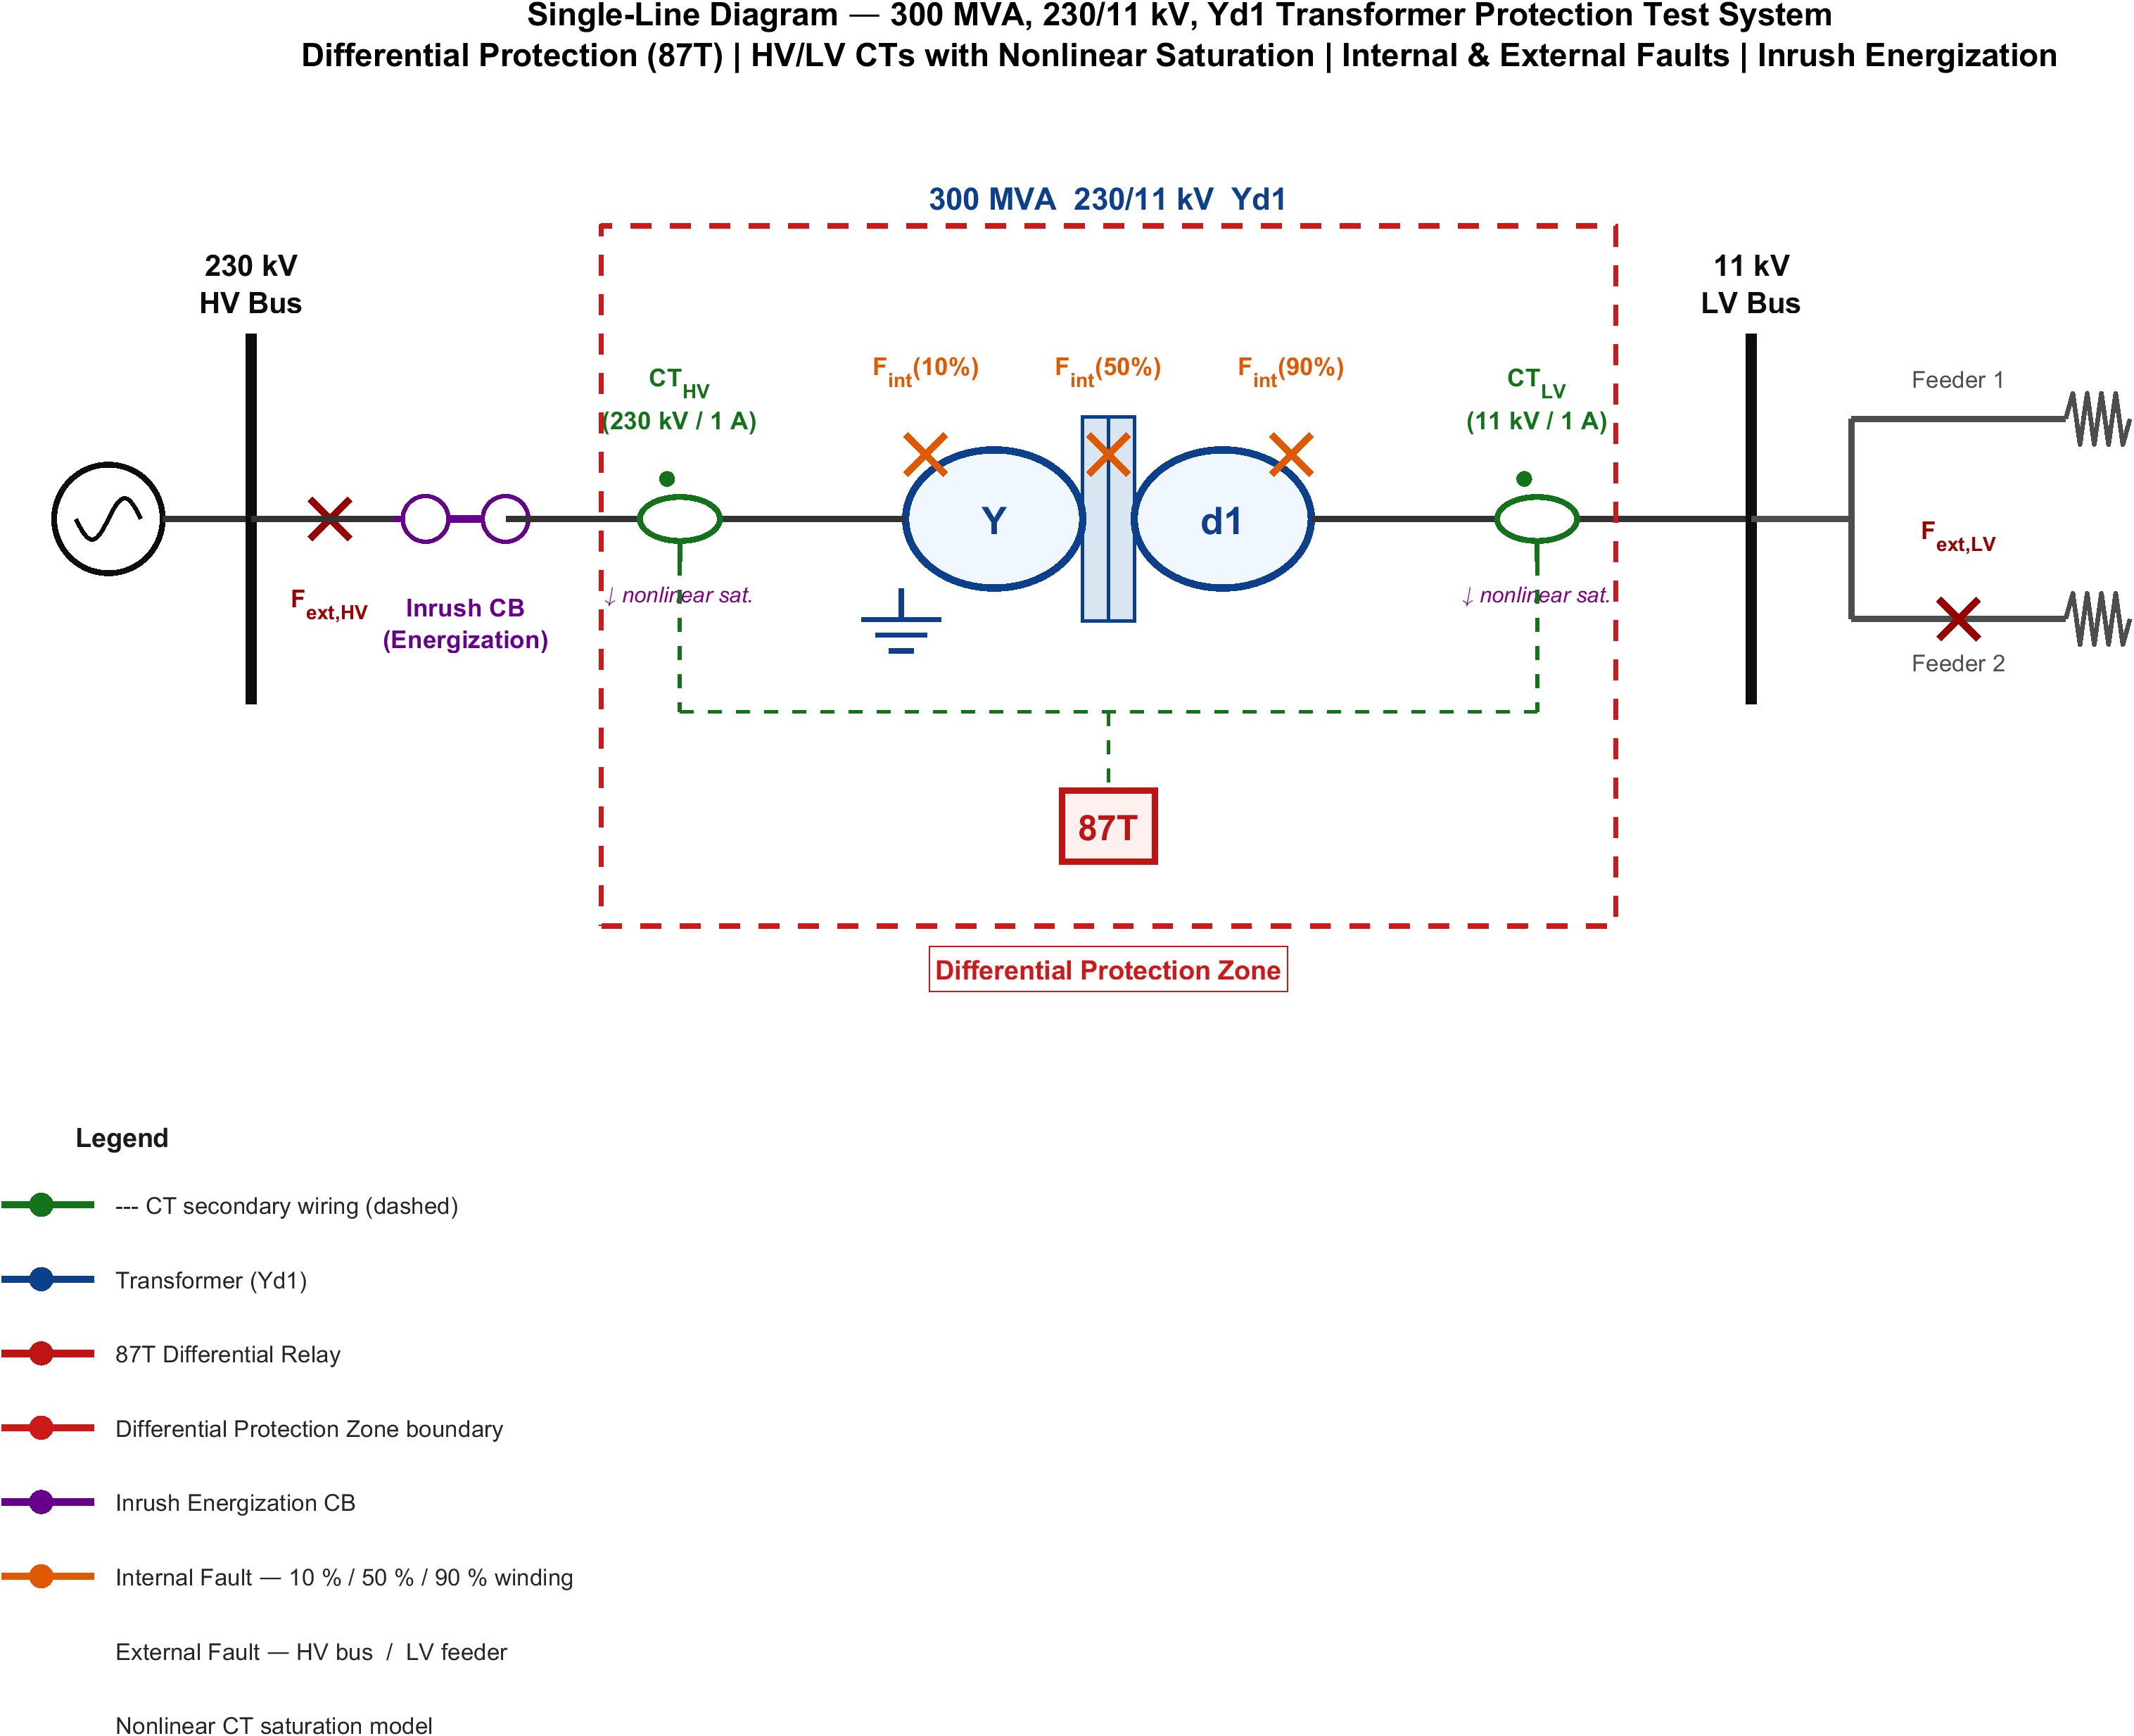
\includegraphics[width=0.6\textwidth]{fig_1_1.png}
\caption{Single-line schematic of the transformer differential protection zone.}\label{fig:1.1}\end{figure}

\section{Research Motivation}
The reliability of differential protection is increasingly threatened by compounding factors. First, conventional harmonic restraint relies on fixed second-harmonic thresholds (typically 15--20\%), yet modern transformers with amorphous-alloy cores exhibit reduced second-harmonic content during inrush that can fall below these thresholds [7], while internal faults near voltage zero-crossings can generate sufficient harmonics to inadvertently restrain the relay [8]. Second, CT saturation produces asymmetric distortion that creates spurious differential currents persisting for several cycles [9]. Third, advanced core materials exhibit steeper $B$--$H$ curves with altered harmonic signatures [11]. Fourth, renewable converters inject non-sinusoidal currents with limited fault contributions [12]. Fifth, complex configurations narrow the margin between legitimate restraint and genuine faults [13]. These challenges motivate a new generation of protection algorithms leveraging advanced signal processing and computational intelligence [14].

\section{Problem Statement}
Despite over a century of development, transformer differential protection schemes continue to experience maloperations at unacceptable rates. \textbf{Given} time-series differential current signals $\{I_d(t)\}$ sampled at $f_s$, encompassing internal faults, magnetizing inrush, external faults with CT saturation, overexcitation, and normal load conditions, corrupted by measurement noise and CT errors; \textbf{find} a classification function $f:\mathcal{X}\!\to\!\mathcal{Y}$ mapping $x\in\mathcal{X}$ to $\mathcal{Y}=\{$Trip, No-Trip$\}$ with high accuracy; \textbf{subject to} operating time within a half-cycle (10\,ms at 50\,Hz), missed-detection probability $P_{miss}\le 0.01$, false-trip probability $P_{false}\le 0.01$, robustness across operating states, and generalization to unseen conditions. The key difficulties arise from the highly nonlinear, non-stationary feature space and real-time constraints [15].

\section{Research Objectives}
\begin{enumerate}[leftmargin=1.6em,itemsep=2pt]
\item \textbf{Simulation model and data generation.} Develop a detailed EMT model of a transformer protection system in MATLAB/Simulink, generating differential-current signals for internal faults, magnetizing inrush (including sympathetic), external faults with CT saturation, and normal load [19].
\item \textbf{Optimal DWT feature extraction.} Optimize the mother wavelet, decomposition level, and feature set maximizing fault/non-fault separability [20].
\item \textbf{Hybrid DWT--LSTM classification and adaptive logic.} Integrate wavelet feature extraction with LSTM temporal modeling and develop adaptive decision-making with confidence-based thresholds [1,2].
\item \textbf{Evaluation, benchmarking, and robustness.} Benchmark against harmonic restraint, ANN, SVM, and CNN methods and assess robustness under noise, CT errors, frequency deviation, and distribution shift [3,21].
\end{enumerate}

\section{Scope and Limitations}
\subsection{Scope}
A two-winding 300\,MVA, 230/11\,kV, Yd1 transformer is modeled in detail; generalization to other ratings and vector groups is future work. Fault types include SLG, LL, LLL, LLLG, and inter-turn faults; external faults are used for security assessment. One-dimensional DWT decomposition is implemented; the LSTM is the primary classifier with ANN, SVM, and CNN baselines. Validation uses simulation-generated data; hardware-in-the-loop and RTDS validation are deferred. The system is configured for 50\,Hz.
\subsection{Limitations}
Training data is simulation-generated; no physical-relay validation is performed; class imbalance is mitigated by augmentation; the adaptive threshold targets static loading; and IEC 61850 communication failures are not considered.

\section{Contributions of This Work}
\textbf{(1)} A systematic wavelet feature-selection framework using Fisher's discriminant ratio and mutual information [22]. \textbf{(2)} A novel serial DWT--LSTM architecture combining localized time-frequency decomposition with long-term temporal modeling, benchmarked across seven methods [1,23]. \textbf{(3)} An adaptive decision framework with confidence-based thresholds and a probabilistic uncertainty layer, validated under noise (20--60\,dB SNR), CT errors ($\pm5\%$), frequency deviation, and distribution shift [2,24].

\section{Thesis Organization}
Chapter~2 reviews the literature and identifies research gaps. Chapter~3 establishes the mathematical foundations. Chapter~4 details the MATLAB/Simulink model and dataset. Chapter~5 presents the DWT--LSTM methodology. Chapter~6 reports results, benchmarking, and robustness. Chapter~7 concludes and outlines future work.

\chapter{Literature Review}
\section{Introduction}
This chapter critically reviews transformer differential protection, spanning conventional harmonic restraint and waveform-based methods, signal-processing techniques, machine-learning approaches (ANN, SVM, PNN, ensembles), and deep-learning architectures (CNN, RNN, LSTM), identifying the research gaps that motivate the proposed hybrid framework. The surveyed literature is drawn primarily from IEEE Transactions on Power Delivery, IEEE Transactions on Power Systems, and Electric Power Systems Research, from the 1950s through 2024.

\section{Conventional Differential Protection Methods}
\subsection{Harmonic Restraint Methods}
The harmonic restraint method, first proposed by Sharp and Glassburn in 1958, is the most widely deployed technique for discriminating inrush from internal faults [7]. Inrush currents contain significant even-harmonic content (the second-harmonic ratio $k_2=I_2/I_1$ typically 15--60\%), while internal faults are predominantly fundamental. The relay trips only when
\begin{equation}
I_d>I_{pickup},\quad I_d>S\,I_r,\quad \frac{I_2}{I_1}<k_{threshold},
\end{equation}
with $k_{threshold}$ typically set between 15\% and 20\%. Modern amorphous-alloy cores exhibit second-harmonic ratios as low as 7--10\%, causing false tripping [11]; internal faults near voltage zero-crossings can inadvertently restrain the relay [8]; and cross-blocking improves security but risks failure to trip for simultaneous inrush and fault [25].
\subsection{Waveform-Based and Equivalent-Circuit Methods}
Dead-angle methods classify an event as inrush when the per-half-cycle interval with current below a threshold exceeds 65--80$^\circ$, but are sensitive to threshold selection, noise, and CT saturation [26]. Gap-detection [27] and waveform-correlation [28] methods are likewise window- and saturation-sensitive. Equivalent-circuit methods detect faults when terminal measurements violate magnetic-circuit equations [29] but require accurate models and voltage measurements [30].

\section{Signal Processing Techniques}
The Discrete Fourier Transform provides frequency resolution at the expense of time localization, limiting its ability to capture transient inrush and fault waveforms [31,32]. The wavelet transform overcomes this through simultaneous time-frequency localization. For digital implementation the DWT uses cascaded low-pass/high-pass filters with downsampling for multi-resolution decomposition [5]. db4 at five levels achieved 97.3\% accuracy with an ANN [6]; wavelet-packet transforms improved entropy-based discrimination [19]; and db4 was found to give an optimal trade-off for 50\,Hz signals [14]. A persistent limitation is that window-wise wavelet features ignore temporal evolution across successive windows.

\section{Machine Learning Approaches}
\textbf{ANNs.} A three-layer MLP with harmonic features achieved 98.5\% accuracy on 2{,}000 simulated events [9], improved to 99.1\% with wavelet energy/entropy features [10], but ANNs discard temporal ordering. \textbf{SVMs.} RBF-kernel SVMs reached 98.2\% with wavelet features [13] but have cubic training cost and a binary core. \textbf{PNNs.} Parzen-window PNNs reached 97.8--98.9\% [9,25] but scale linearly with samples. \textbf{Ensembles.} Random forests on Fourier+wavelet features reached 99.0\% [11] at the cost of interpretability.

\section{Deep Learning Approaches}
\subsection{CNN, RNN, and LSTM Architectures}
A 1D-CNN at 1\,kHz over two-cycle windows reached 98.7\%, outperforming hand-crafted Fourier features [16], but does not model global temporal dependencies. RNNs maintain a hidden state but suffer vanishing gradients; the LSTM overcomes this through a gated cell:
\begin{align}
f_t&=\sigma(W_f[h_{t-1},x_t]+b_f), & i_t&=\sigma(W_i[h_{t-1},x_t]+b_i),\\
\tilde{C}_t&=\tanh(W_C[h_{t-1},x_t]+b_C), & C_t&=f_t\odot C_{t-1}+i_t\odot \tilde{C}_t,\\
o_t&=\sigma(W_o[h_{t-1},x_t]+b_o), & h_t&=o_t\odot\tanh(C_t),
\end{align}
where $\sigma$ is the sigmoid and $\odot$ the Hadamard product. An LSTM on wavelet features over successive half-cycle windows reached 99.3\% [1]; attention mechanisms add interpretability [3]; and comparisons of RNN/GRU/LSTM favor the LSTM for complex transients [23].
\subsection{Emerging Architectures}
Autoencoders enable unsupervised anomaly detection [35]; GANs augment synthetic data [36]; and Transformers, though promising, face quadratic scaling that challenges real-time use [37].

\section{Comparative Synthesis of the Literature}
Table~\ref{tab:litcompare} synthesizes representative studies. Reported accuracies are the authors' own on their own datasets and are not directly comparable; a controlled comparison on a single unified dataset is given in Chapter~6.
\begin{table}[H]\centering
\caption{Comparative synthesis of representative transformer differential protection studies.}\label{tab:litcompare}
\small
\begin{tabular}{@{}clp{5.2cm}cl@{}}
\toprule
\textbf{Ref.} & \textbf{Approach} & \textbf{Classifier / method} & \textbf{Acc.\,(\%)} & \textbf{Limitation}\\ \midrule
{[6]} & db4 DWT & Threshold logic & $\sim$97 & Hand-tuned thresholds\\
{[19]} & DWT & Back-propagation NN & $\sim$97 & Static feature vector\\
{[18]} & Wavelet stats & ANN & 99.1 & No temporal context\\
{[9]} & Harmonic & Optimal PNN & 97.8 & Memory grows with samples\\
{[13]} & Wavelet & SVM (RBF) & 98.2 & No sequence modelling\\
{[20]} & Wavelet packet & SVM & $\sim$98 & High dimensionality\\
{[11]} & Fourier+wavelet & Random forest & 99.0 & No temporal model\\
{[16]} & Accelerated DNN & 1D-CNN & 98.7 & Weak long-range context\\
{[3]} & Wavelet & LSTM & 99.3 & No hybrid relay handshake\\
{[1,2]} & Improved wavelet & LSTM & $\sim$99.5 & No supervisory veto\\
{[23]} & Dual DNN & Inrush vs.\ internal & $\sim$99.4 & Two-class only\\
\textbf{This work} & 3-level db4 energy & LSTM (attention) + 87T veto & \textbf{98.89/100} & ---\\
\bottomrule
\end{tabular}
\end{table}
The field has progressed from fixed-threshold schemes through shallow learning to deep sequence models, with accuracy rising above 99\%. Yet almost all recent high-accuracy studies evaluate a standalone classifier that issues the trip directly, leaving the dependability--security trade-off implicit, and none couples the learned classifier to a certified 87T element through an explicit supervisory handshake. This thesis is distinguished on all three counts.

\section{Research Gaps}
Five gaps motivate this work: (1) ad-hoc wavelet parameter selection; (2) no full integration of DWT feature extraction with LSTM temporal modeling in a serial hybrid; (3) fixed decision thresholds; (4) limited robustness evaluation; and (5) absence of standardized benchmarking. This thesis addresses all five.

\chapter{Mathematical Modeling and Theoretical Framework}
\section{Introduction}
This chapter establishes the mathematical foundations for the proposed DWT--LSTM scheme: differential relaying principles, magnetizing inrush theory, CT saturation modeling, internal-fault characteristics, and the classification framework.

\section{Transformer Differential Protection Fundamentals}
\subsection{Differential and Restraint Currents}
For a two-winding transformer,
\begin{equation}
I_d=\bigl|\dot{I}_1 N_1+\dot{I}_2 N_2\bigr|,\qquad
I_r=\tfrac{1}{2}\bigl(|\dot{I}_1 N_1|+|\dot{I}_2 N_2|\bigr),
\end{equation}
where $\dot{I}_1,\dot{I}_2$ are phasor currents referred to a common level. Under healthy conditions $I_d\approx0$; a small residual arises from CT mismatch, tap changes, magnetizing current, and measurement errors:
\begin{equation}
I_{d,steady}=\sqrt{(\varepsilon_{CT}I_{load})^2+(\Delta_{tap}I_{load})^2+I_m^2+\varepsilon_{meas}^2}.
\end{equation}
\subsection{Operating Characteristics}
The dual-slope restraint characteristic defines the operating threshold $I_{op}$ as a function of $I_r$, with first slope $S_1$ (25--40\%) accommodating steady-state errors and second slope $S_2$ (50--80\%) providing restraint during CT saturation; the relay trips when $I_d>I_{op}$.
\begin{figure}[H]\centering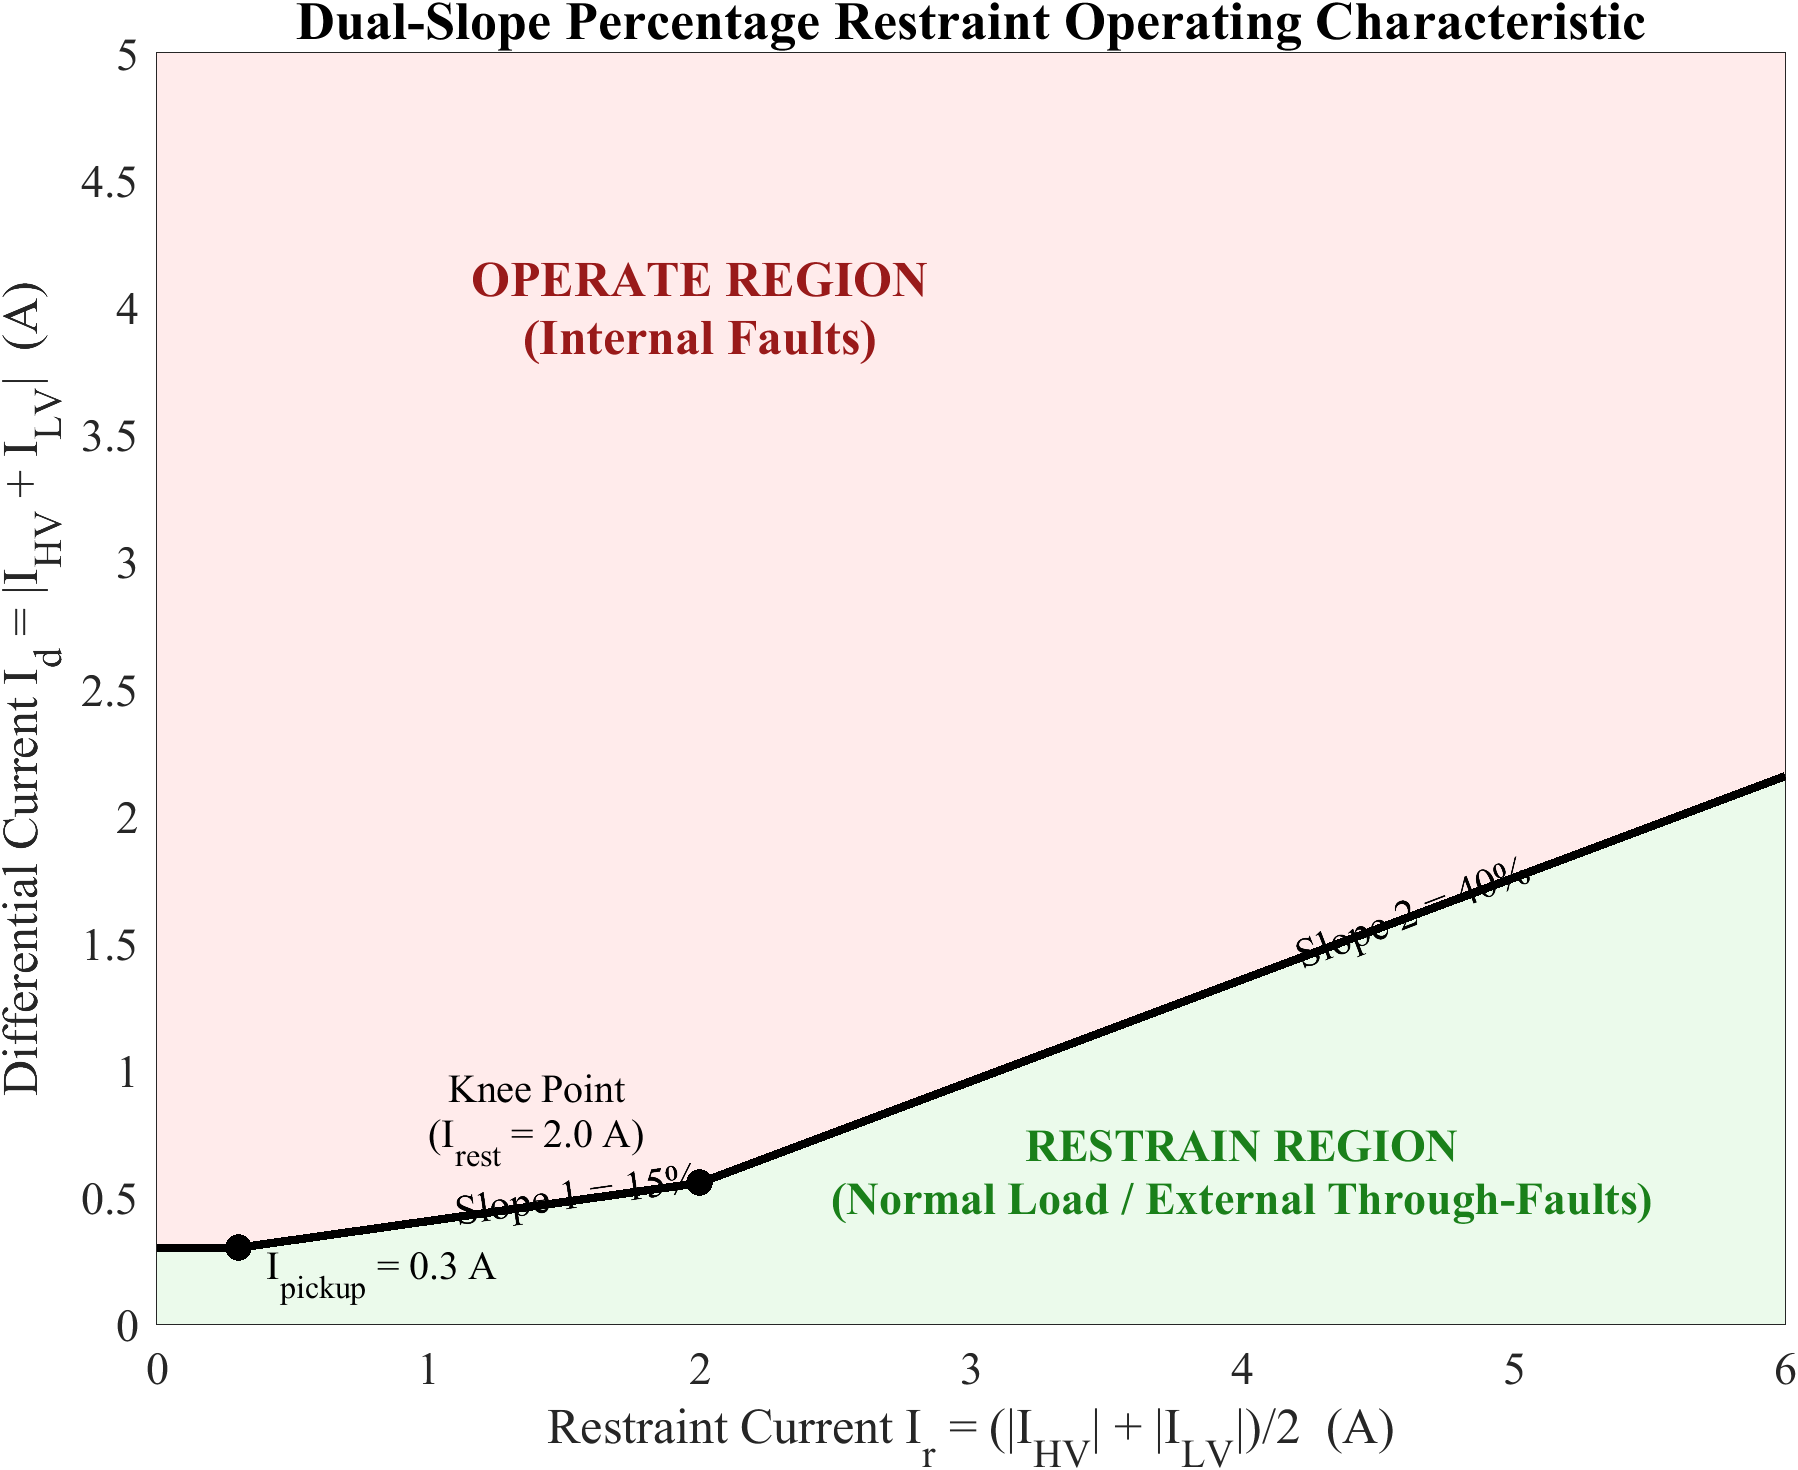
\includegraphics[width=0.55\textwidth]{fig_3_1.png}
\caption{Dual-slope percentage restraint characteristic of the differential relay.}\label{fig:3.1}\end{figure}
\subsection{Pickup Current}
The pickup balances sensitivity and security, $I_{d,steady,max}<I_{pickup}<I_{d,fault,min}$, typically 0.2--0.5\,pu, with minimum detectable SLG fault current $I_{f,min}=I_{pickup}/[1-R_f/(Z_{s}+Z_{t})]$.

\section{Magnetizing Inrush Current}
\subsection{Core Saturation Theory}
Faraday's law gives $v(t)=N\,d\phi/dt=NA\,dB/dt$. For $v(t)=V_m\sin(\omega t+\alpha)$, including the DC transient,
\begin{equation}
\phi(t)=-\Phi_m\cos(\omega t+\alpha)+\Phi_m\cos(\alpha)e^{-t/\tau}+\Phi_r e^{-t/\tau}.
\end{equation}
At worst-case energization ($\alpha=0,\ \Phi_r=\Phi_m$), $\Phi_{peak}=2\Phi_m+\Phi_r=3\Phi_m$, exceeding $B_{sat}$ and causing severe saturation.
\begin{figure}[H]\centering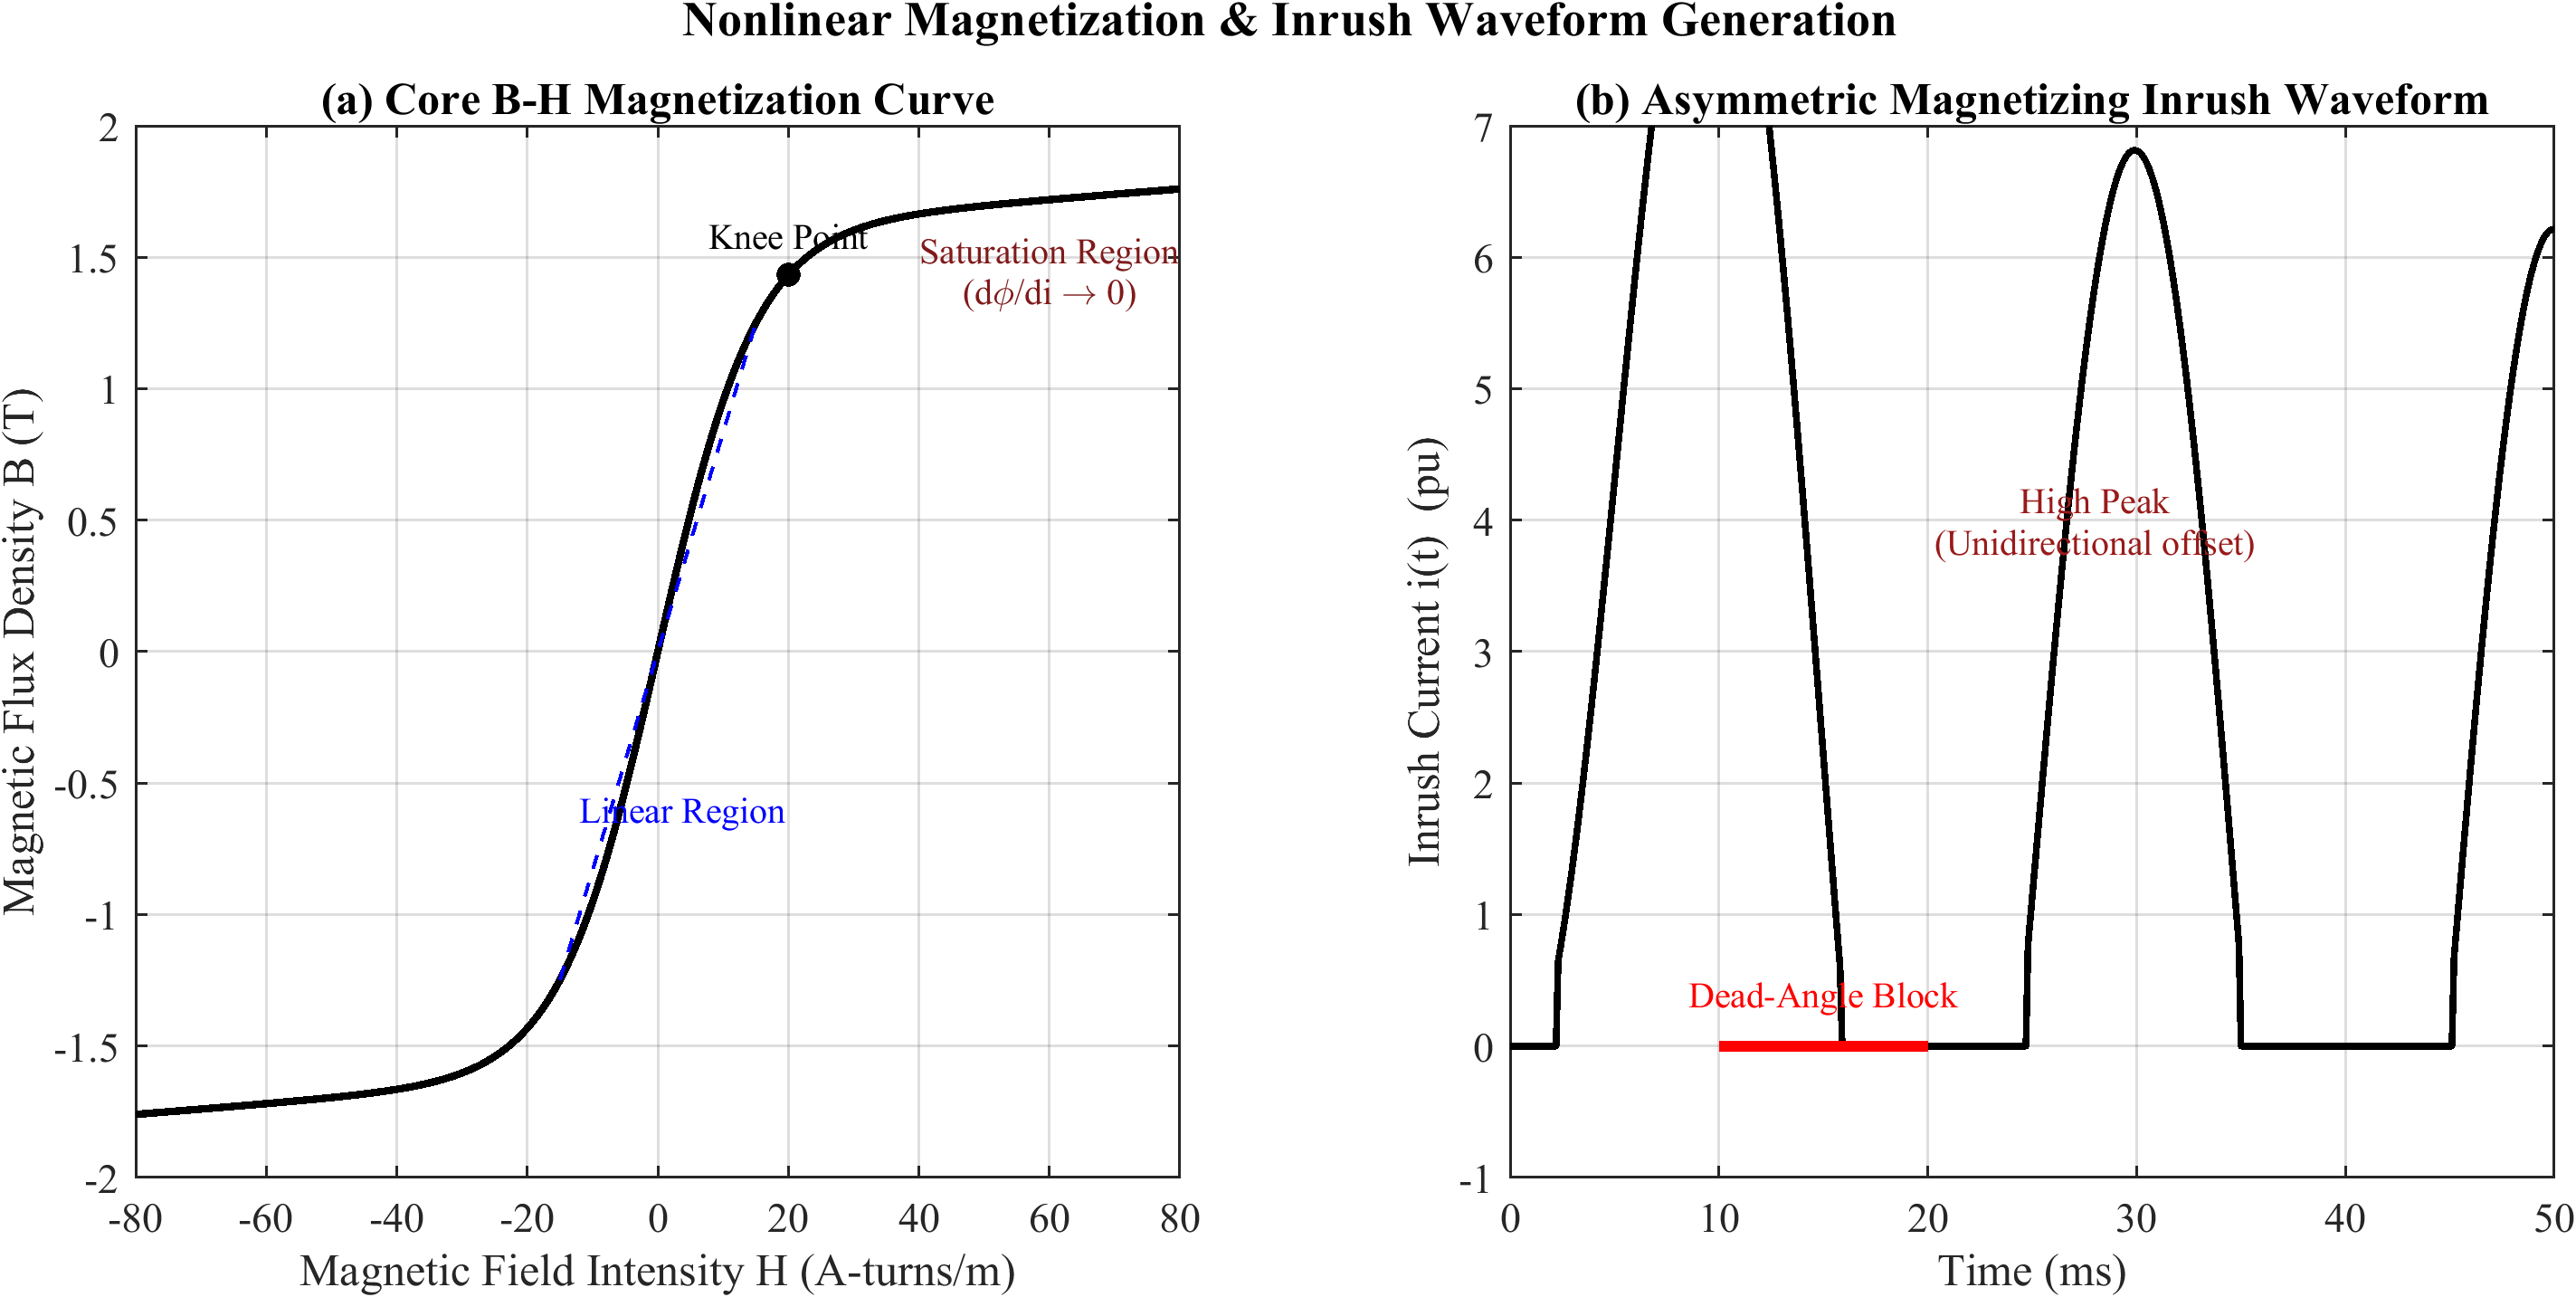
\includegraphics[width=0.85\textwidth]{fig_3_2.png}
\caption{Core $B$--$H$ saturation curve and the resulting magnetizing inrush waveform.}\label{fig:3.2}\end{figure}
\subsection{Factors and Harmonics}
Inrush magnitude depends on switching angle $\alpha$, residual flux $\Phi_r$ (0--80\% of $\Phi_m$), source impedance, and core material, ranging 3--15$\times$ rated current. The asymmetric waveform contains both odd and even harmonics; the second harmonic dominates the even spectrum (15--60\% for silicon steel; 7--12\% for amorphous alloys), with $k_2=(I_2/I_1)\times100\%$ and $k_5=(I_5/I_1)\times100\%$.
\subsection{Sympathetic Inrush}
Sympathetic inrush occurs when an energizing transformer's DC inrush, flowing through the common source impedance, drives an already-energized parallel transformer into opposite-polarity saturation, producing a slowly decaying differential current that can persist for tens of seconds [4].

\section{Current Transformer Saturation}
The CT secondary current equals the referred primary minus the excitation current, $I_s=I_p'-I_e$, with $I_e=V_s/(R_m+jX_m)$. The nonlinear magnetization curve uses $i_e(\lambda)=Ae^{B|\lambda|}\operatorname{sign}(\lambda)+C\lambda$, with $\lambda=N_2\phi$. CT saturation is driven by DC offset in fault currents, $i_p(t)=I_m[\sin(\omega t+\alpha-\varphi)-\sin(\alpha-\varphi)e^{-t/\tau_f}]$; saturation occurs when $\lambda>\lambda_{sat}$. Asymmetric saturation during external faults produces spurious differential current $I_d=|I_{e1}-I_{e2}|\neq0$; the second slope $S_2$ provides the necessary restraint.
\begin{figure}[H]\centering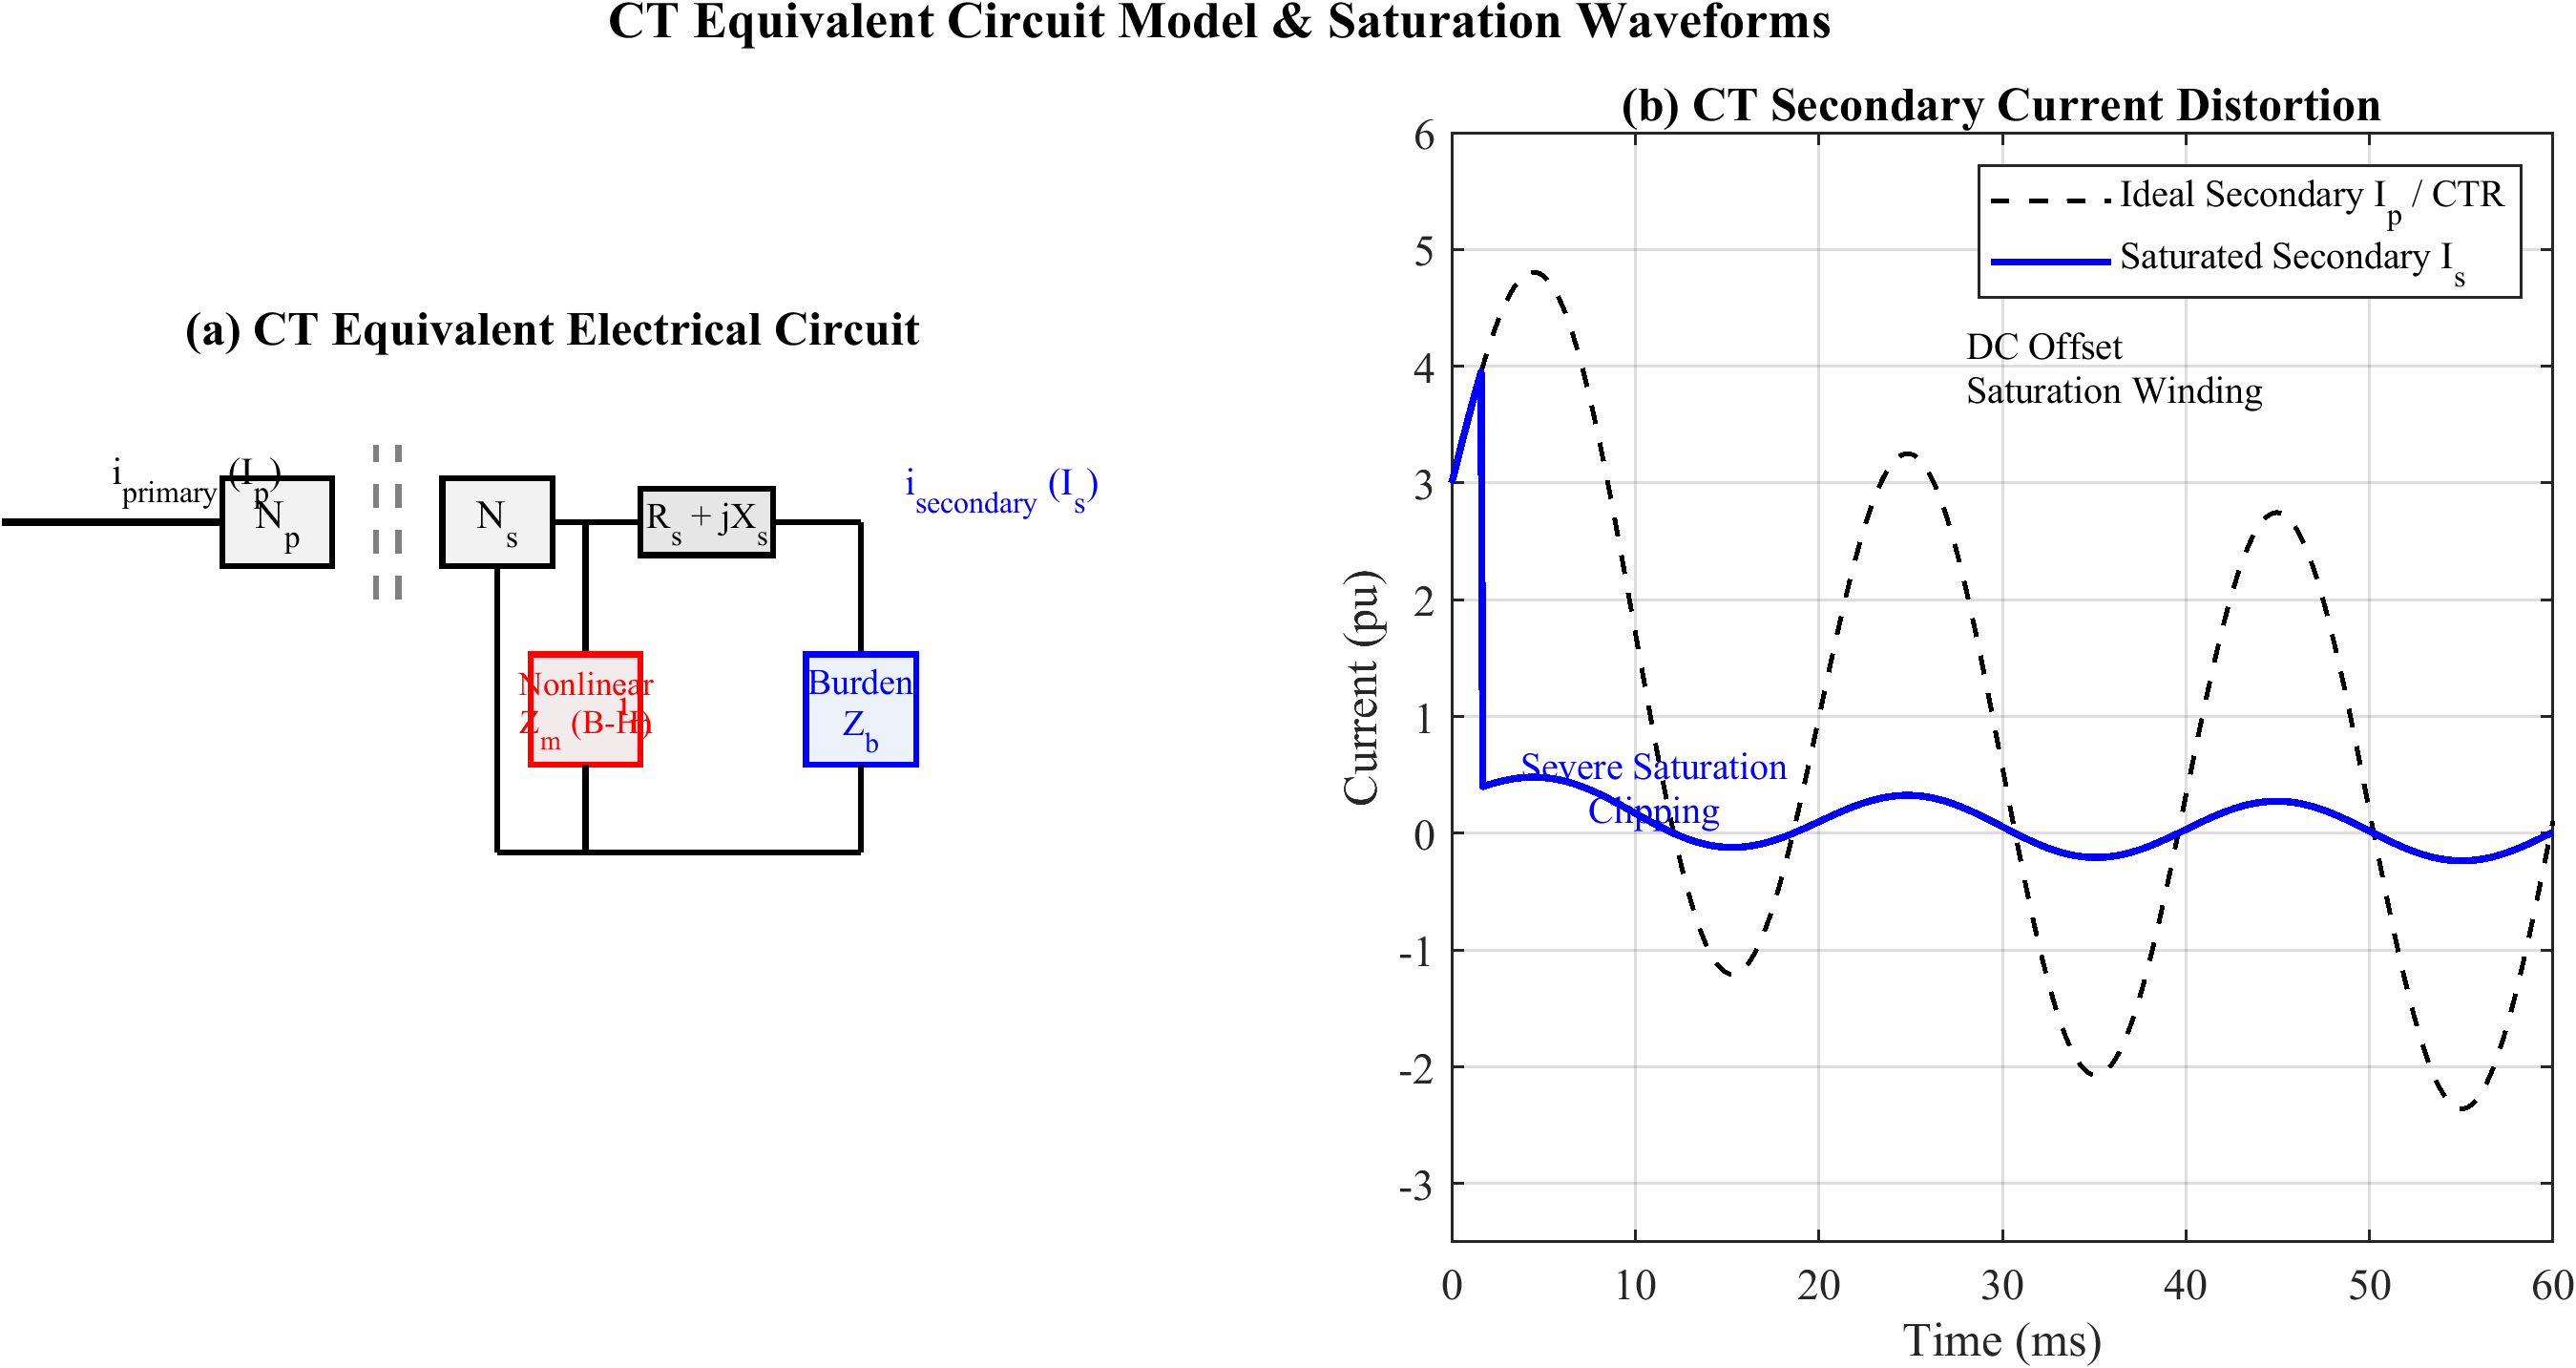
\includegraphics[width=0.85\textwidth]{fig_3_3.png}
\caption{Current transformer equivalent circuit and saturation-induced secondary distortion.}\label{fig:3.3}\end{figure}

\section{Internal Fault Characteristics}
Internal faults include SLG (most common), LL, LLL/LLLG, and inter-turn faults. Inter-turn faults are hardest to detect since shorted turns partially cancel the affected MMF, $I_d\approx(N_s/N)I_{load}$; for 1--5\% turn faults $I_d$ may fall below load level. Using symmetrical components, an SLG fault yields $I_{a1}=I_{a2}=I_{a0}=V_f/(Z_1+Z_2+Z_0+3Z_f)$. Fault time constants (0.02--0.05\,s) are shorter than inrush (0.1--0.5\,s), with lower even-harmonic content.

\section{Mathematical Framework for Classification}
\subsection{Feature Space and Bayes-Optimal Decision}
The wavelet energy at level $k$ is $E_{Dk}=\sum_n|d_k[n]|^2$. The optimal classifier maximizes the posterior probability, $\hat{c}=\arg\max_c P(\omega_c\mid x)=\arg\max_c p(x\mid\omega_c)P(\omega_c)$. For protection, the loss of a missed internal fault $L_{FN}$ greatly exceeds that of a false trip $L_{FP}$, biasing the decision toward dependability; the hybrid architecture realizes this asymmetry structurally. The LSTM learns the mapping through a softmax output and cross-entropy loss:
\begin{equation}
P(\omega_c\mid x_{1:T})=\frac{e^{z_c}}{\sum_k e^{z_k}},\qquad
\mathcal{L}=-\frac{1}{N}\sum_{n}\sum_{c} y_{n,c}\ln P(\omega_c\mid x_{1:T}^{(n)}).
\end{equation}
Feature separability is guided by the Fisher discriminant ratio $\text{FDR}=(\mu_{c1}-\mu_{c2})^2/(\sigma_{c1}^2+\sigma_{c2}^2)$ and by the mutual information $I(X;Y)=H(Y)-H(Y\mid X)$.
\begin{figure}[H]\centering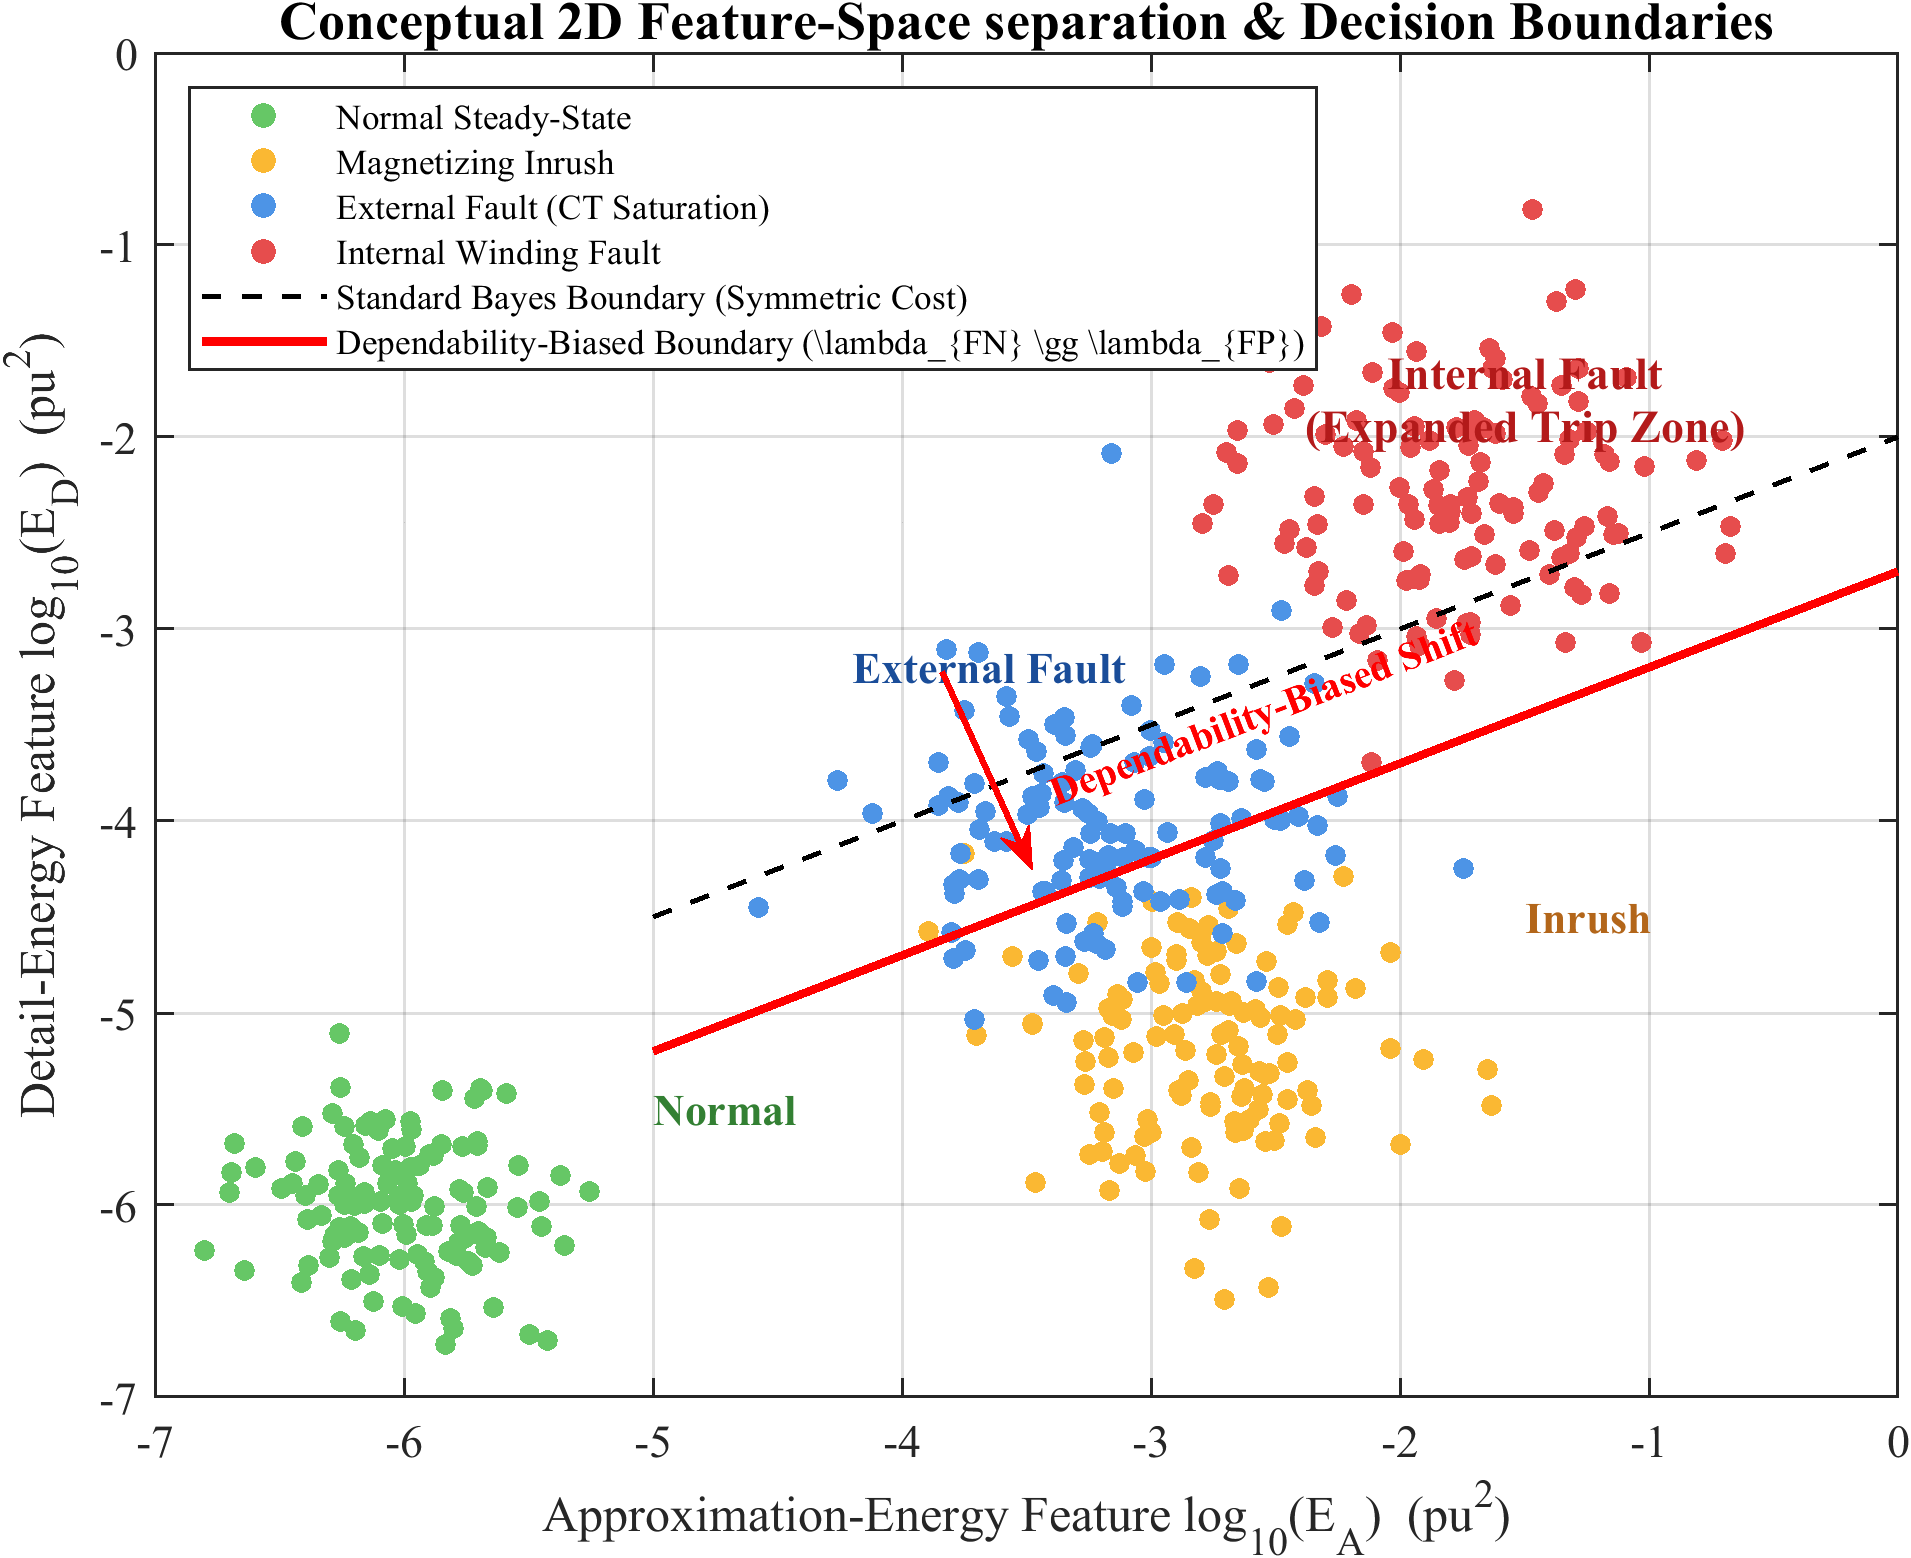
\includegraphics[width=0.55\textwidth]{fig_3_4.png}
\caption{Conceptual feature-space separation of the event classes with cost-asymmetric decision boundaries.}\label{fig:3.4}\end{figure}
\subsection{Performance Metrics}
Performance is evaluated by accuracy, precision $=TP/(TP+FP)$, recall $=TP/(TP+FN)$, and $F1=2\,P\,R/(P+R)$. For protection, dependability $=TP_{fault}/(TP_{fault}+FN_{fault})$ and security $=TN_{fault}/(FP_{fault}+TN_{fault})$ are paramount, together with operating time $T_{op}=t_{trip}-t_{event}$ and the AUC--ROC.
\subsection{Adaptive Pickup}
An adaptive pickup tracks the operating state, $I_{pickup}(t)=I_{p0}+k_1 I_r(t)+k_2\hat{\sigma}_d(t)$, where $k_1 I_r$ reproduces the percentage slope and $k_2\hat{\sigma}_d$ inflates the threshold transiently when CT saturation or noise elevates the differential-current variance.

\chapter{Power System Simulation Model Using MATLAB/Simulink}
\section{Introduction}
MATLAB/Simulink was selected for its integrated environment combining high-fidelity electromagnetic-transient (EMT) modeling via Simscape Electrical with native machine-learning support and ONNX runtime, enabling a seamless workflow from data generation to DWT--LSTM training, validation, and deployment [1,2].
\begin{figure}[H]\centering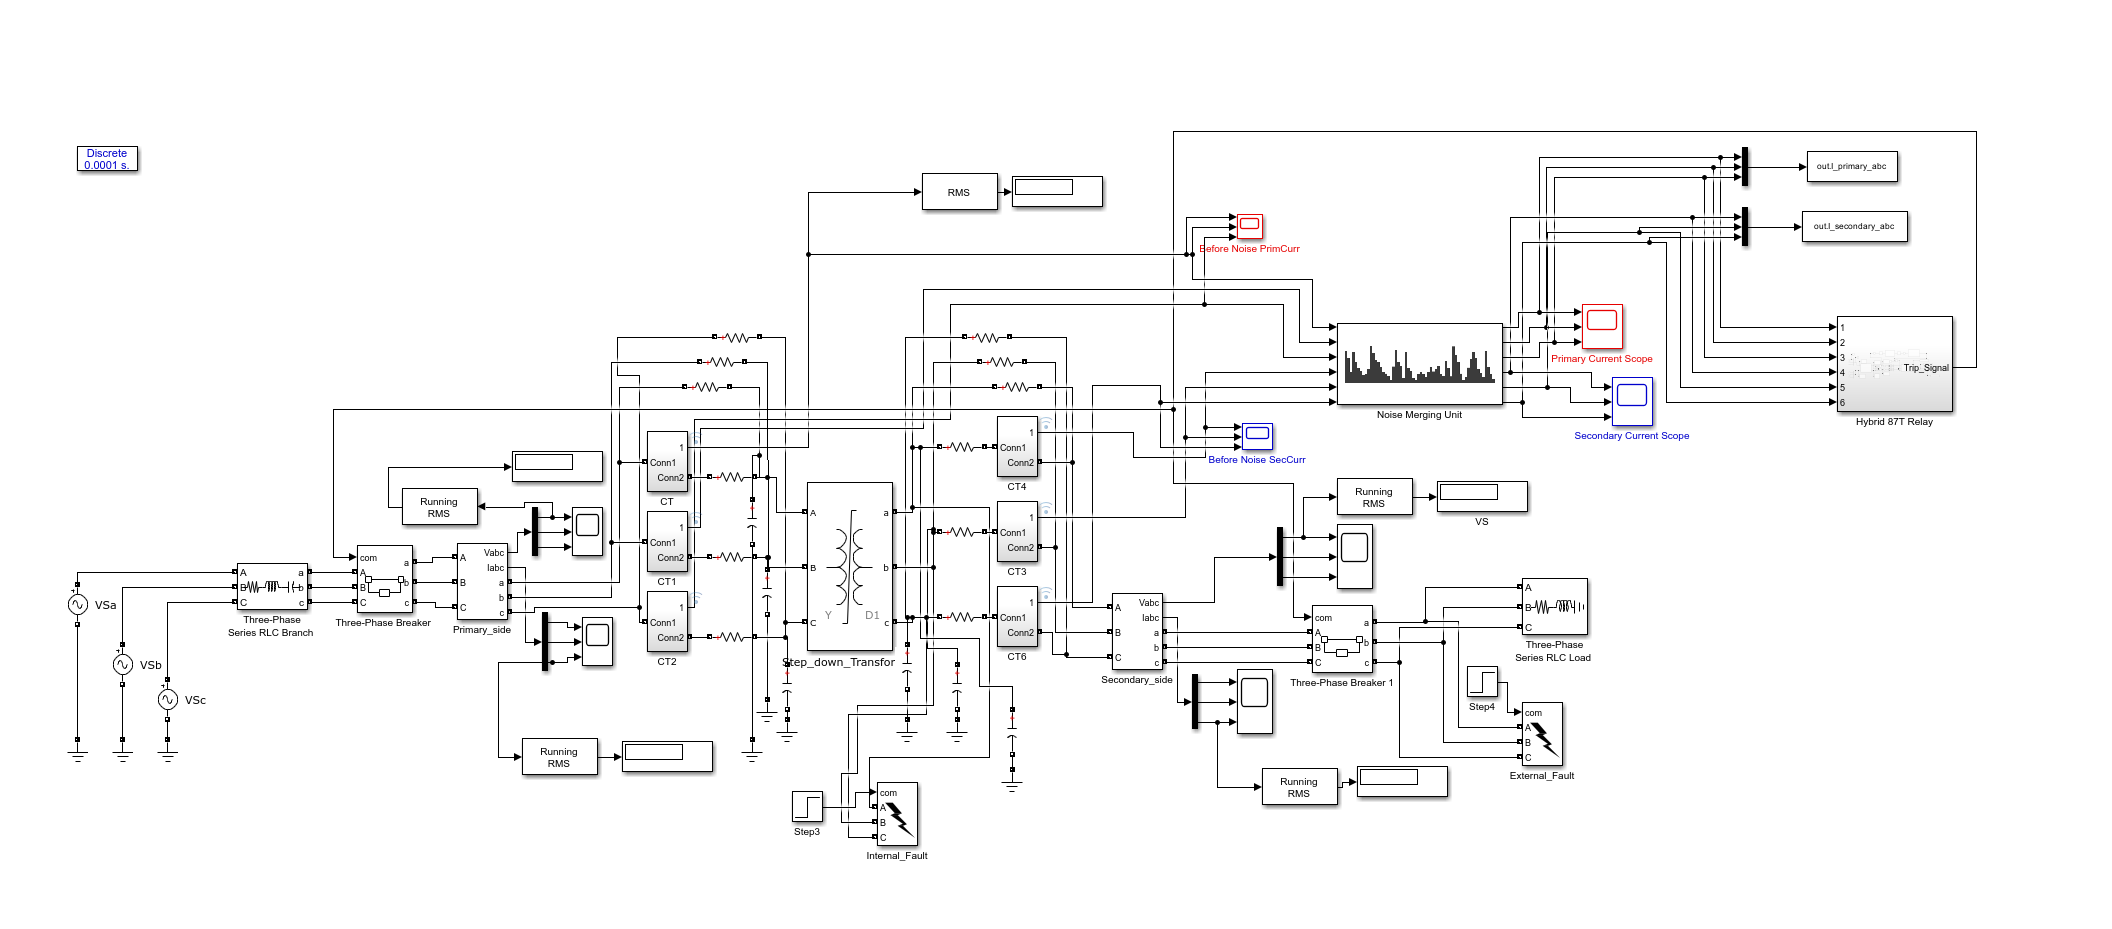
\includegraphics[width=0.95\textwidth]{fig_4_1.png}
\caption{Overview of the MATLAB/Simulink power-system simulation model (Simulink main panel).}\label{fig:4.1}\end{figure}

\section{Simulation Environment}
The platform comprises MATLAB R2024a with Simulink, Simscape Electrical, the Deep Learning Toolbox, the Signal Processing Toolbox, and the ONNX converter. A discrete-time solver with fixed step $\Delta t=1\times10^{-5}$\,s (10\,\textmu s) is used, giving a Nyquist frequency $f_{Nyquist}=1/(2\Delta t)=50$\,kHz---a 50$\times$ oversampling margin over the 1.6\,kHz relay rate. Each simulation runs for $T_{sim}=1.0$\,s with the event injected at $t_{event}=0.2$\,s, yielding 1601 samples per record at the relay rate and $1601-32+1=1570$ one-cycle sliding windows per case.

\section{Transformer Model Parameters}
The protected transformer is a three-phase 300\,MVA, 230/11\,kV unit with Yd1 vector group (grounded wye primary, delta secondary, $-30^\circ$ displacement). Full-load currents are $I_{FLA,HV}=753.1$\,A and $I_{FLA,LV}=15{,}746$\,A; base impedances are $176.33\,\Omega$ (HV) and $0.4033\,\Omega$ (LV). The saturable core uses a piecewise-linear $B$--$H$ curve (20 points, knee near 1.2\,pu); worst-case inrush ($\alpha=0^\circ$, $\phi_r=+\phi_m$) yields $\phi_{peak}=3\phi_m$. The $-30^\circ$ displacement is compensated by a Clarke rotation of the LV-side CT currents.
\begin{table}[H]\centering\caption{Transformer nameplate and equivalent-circuit parameters.}\label{tab:4.1}
\begin{tabular}{@{}lc@{}}\toprule \textbf{Parameter} & \textbf{Value}\\ \midrule
Nominal power $S_{nom}$ & 300\,MVA\\
Primary / secondary voltage & 230\,kV / 11\,kV (L--L)\\
Frequency & 50\,Hz\\
Vector group & Yd1 (Wye/Delta, $30^\circ$ lag)\\
Winding 1 (HV) $R_1$, $L_1$ & 0.0025\,pu, 0.08\,pu\\
Winding 2 (LV) $R_2$, $L_2$ & 0.003\,pu, 0.08\,pu\\
Magnetizing branch $R_m$, $L_m$ & 500\,pu, 5\,pu\\ \bottomrule
\end{tabular}\end{table}

\section{Power System Network and CT Model}
The external system is represented by Th\'evenin equivalents: $Z_{th,HV}=0.5+j15.0\,\Omega$ (SCL 3524\,MVA) and $Z_{th,LV}=0.01+j0.10\,\Omega$ (SCL 1204\,MVA), giving available fault currents of 8.84\,kA (HV) and 63.2\,kA (LV). Breakers use $R_{on}=0.001\,\Omega$ with RC snubbers; the LV load is 240\,MVA at 0.85 pf (80\% loading). CTs on both sides use a saturable core (Table~\ref{tab:4.2}).
\begin{table}[H]\centering\caption{Current transformer parameters.}\label{tab:4.2}
\begin{tabular}{@{}lcc@{}}\toprule \textbf{Parameter} & \textbf{HV Side} & \textbf{LV Side}\\ \midrule
CT ratio & 20:1 & 20:1\\
Accuracy class & 5P20 & 5P20\\
Rated primary current & 753.1\,A & 15{,}746\,A\\
Secondary resistance $R_s$ & 0.5\,$\Omega$ & 0.3\,$\Omega$\\
Burden impedance $Z_b$ & 1.5\,$\Omega$ & 1.0\,$\Omega$\\
Core relative permeability & 2000 & 2000\\ \bottomrule
\end{tabular}\end{table}

\section{Fault and Event Scenarios}
Internal faults are simulated at five winding taps (5--95\%) for four fault types (SLG, LL, LLG, 3LG) with three inception angles and three fault resistances ($Z_{fault}(p)=p^2 Z_k+R_f$), giving 720 deterministic cases. External faults on both buses, including evolving faults and asymmetric CT saturation, give 540 cases. Inrush is generated by sweeping switching angle ($0$--$180^\circ$) and residual flux ($-0.8$ to $+0.8$\,pu), with sympathetic inrush via two parallel transformers, giving 189 cases. CT-saturation stress cases (108) vary burden, fault current, and remanent flux. Normal operation (270 cases) covers six load levels, three taps, five voltages, and three power factors.

\section{Signal Conditioning and Dataset Summary}
Each record passes through a merging-unit chain emulating IEC 61850-9-2: a 4th-order Butterworth anti-alias filter (800\,Hz), 16-bit quantization, and AWGN at 20/30/40\,dB SNR, decimated to 1.6\,kHz. The base corpus comprises 2{,}500 simulated cases with 100\% simulation success and an internal-fault (Trip) prevalence of 41.4\%; a No-Trip positive-class weight of 1.4155 is used in the weighted loss. The fault-resistance range spans 0.001--99\,$\Omega$, inception angle 0--360$^\circ$, and eleven fault types are represented.
\begin{figure}[H]\centering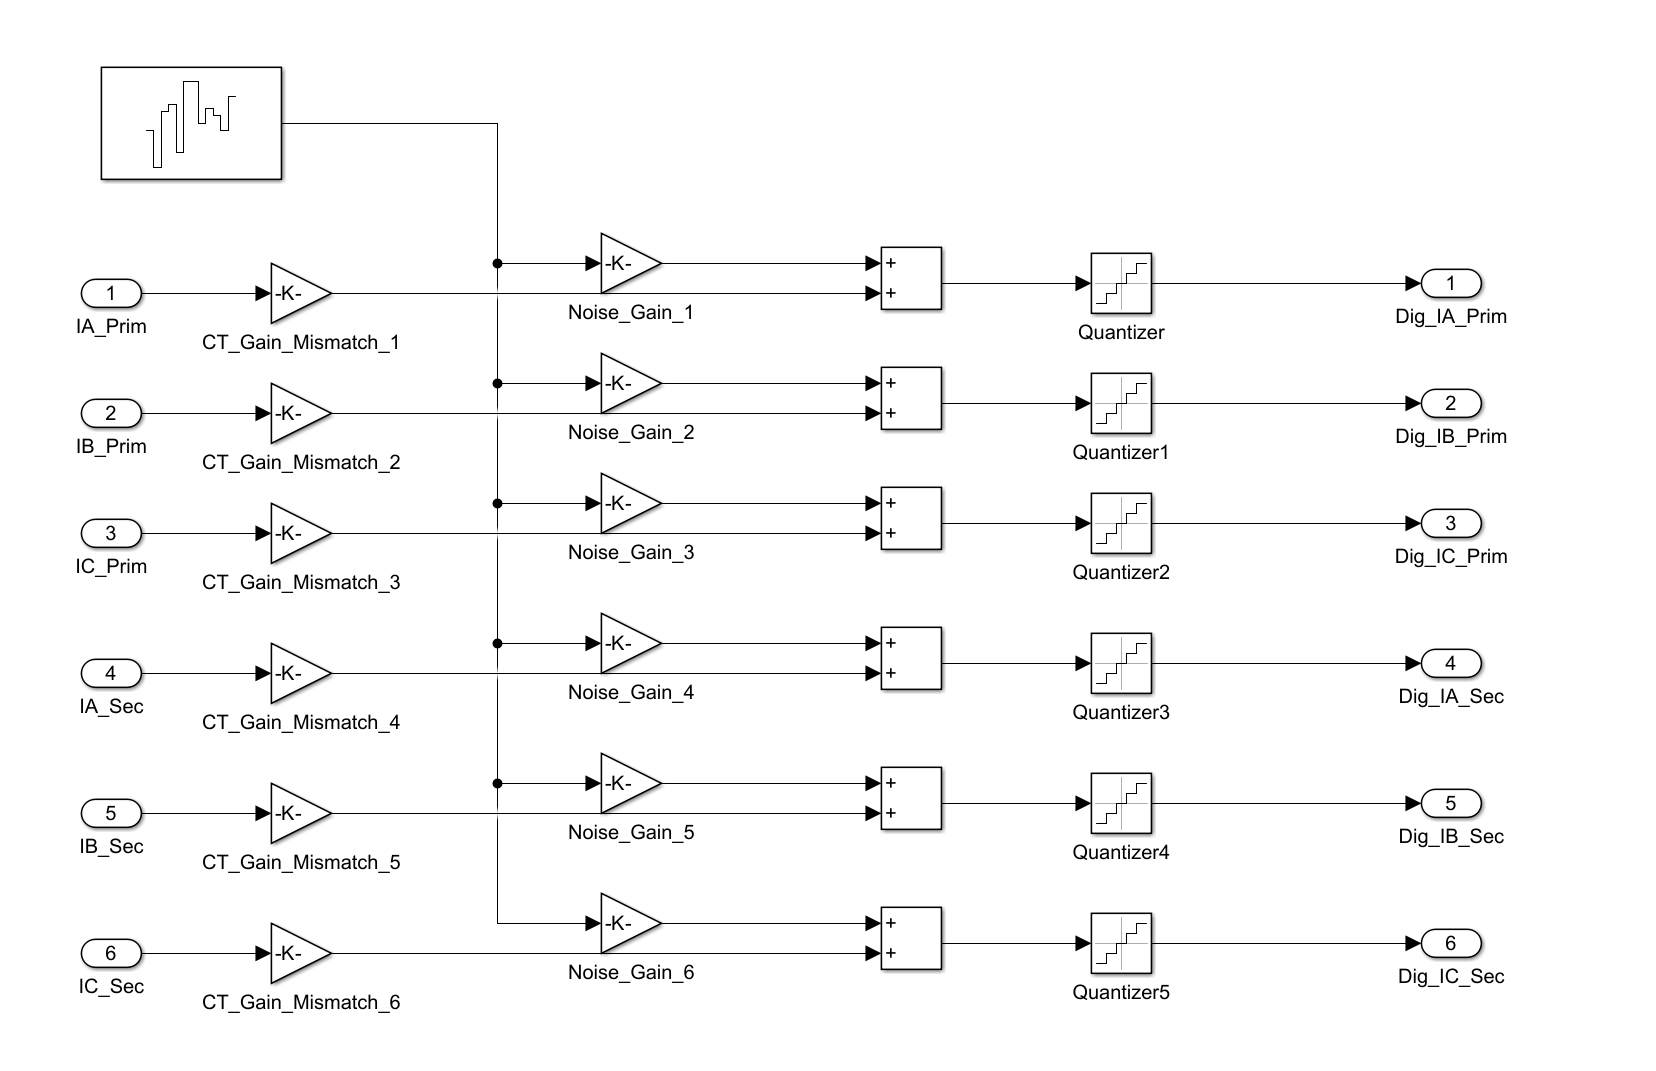
\includegraphics[width=0.7\textwidth]{fig_4_2.png}
\caption{Merging-unit signal-conditioning and noise-injection pipeline.}\label{fig:4.2}\end{figure}
Table~\ref{tab:4.3} summarizes the dataset by event category; the four categories map to a binary protection label (internal $\to$ Trip; external, inrush, normal $\to$ No-Trip). After augmentation and stratified 70/15/15 splitting, the held-out test set comprises 1{,}800 cases.
\begin{table}[H]\centering\caption{Composition of the 2{,}500-case base dataset by event category and protection label.}\label{tab:4.3}
\begin{tabular}{@{}lccc@{}}\toprule \textbf{Event category} & \textbf{Count} & \textbf{Share (\%)} & \textbf{Protection label}\\ \midrule
Internal fault & 1{,}035 & 41.4 & Trip\\
External fault & 578 & 23.1 & No-Trip\\
Magnetizing inrush & 500 & 20.0 & No-Trip\\
Normal operation & 387 & 15.5 & No-Trip\\ \midrule
Total & 2{,}500 & 100.0 & 1{,}035 Trip / 1{,}465 No-Trip\\ \bottomrule
\end{tabular}\end{table}
\begin{table}[H]\centering\caption{Stochastic augmentation parameter ranges.}\label{tab:4.5}
\begin{tabular}{@{}lll@{}}\toprule \textbf{Parameter} & \textbf{Distribution} & \textbf{Range}\\ \midrule
Fault inception angle & Uniform & 0--360$^\circ$\\
Fault resistance & Log-uniform & 0.001--99\,$\Omega$\\
Source impedance variation & Uniform & $\pm5\%$\\
Fault location (winding) & Uniform & 2--98\%\\
Residual flux & Uniform & $-0.8$ to $+0.8$\,pu\\
Loading level & Uniform & 0--110\% rated\\ \bottomrule
\end{tabular}\end{table}
\begin{figure}[H]\centering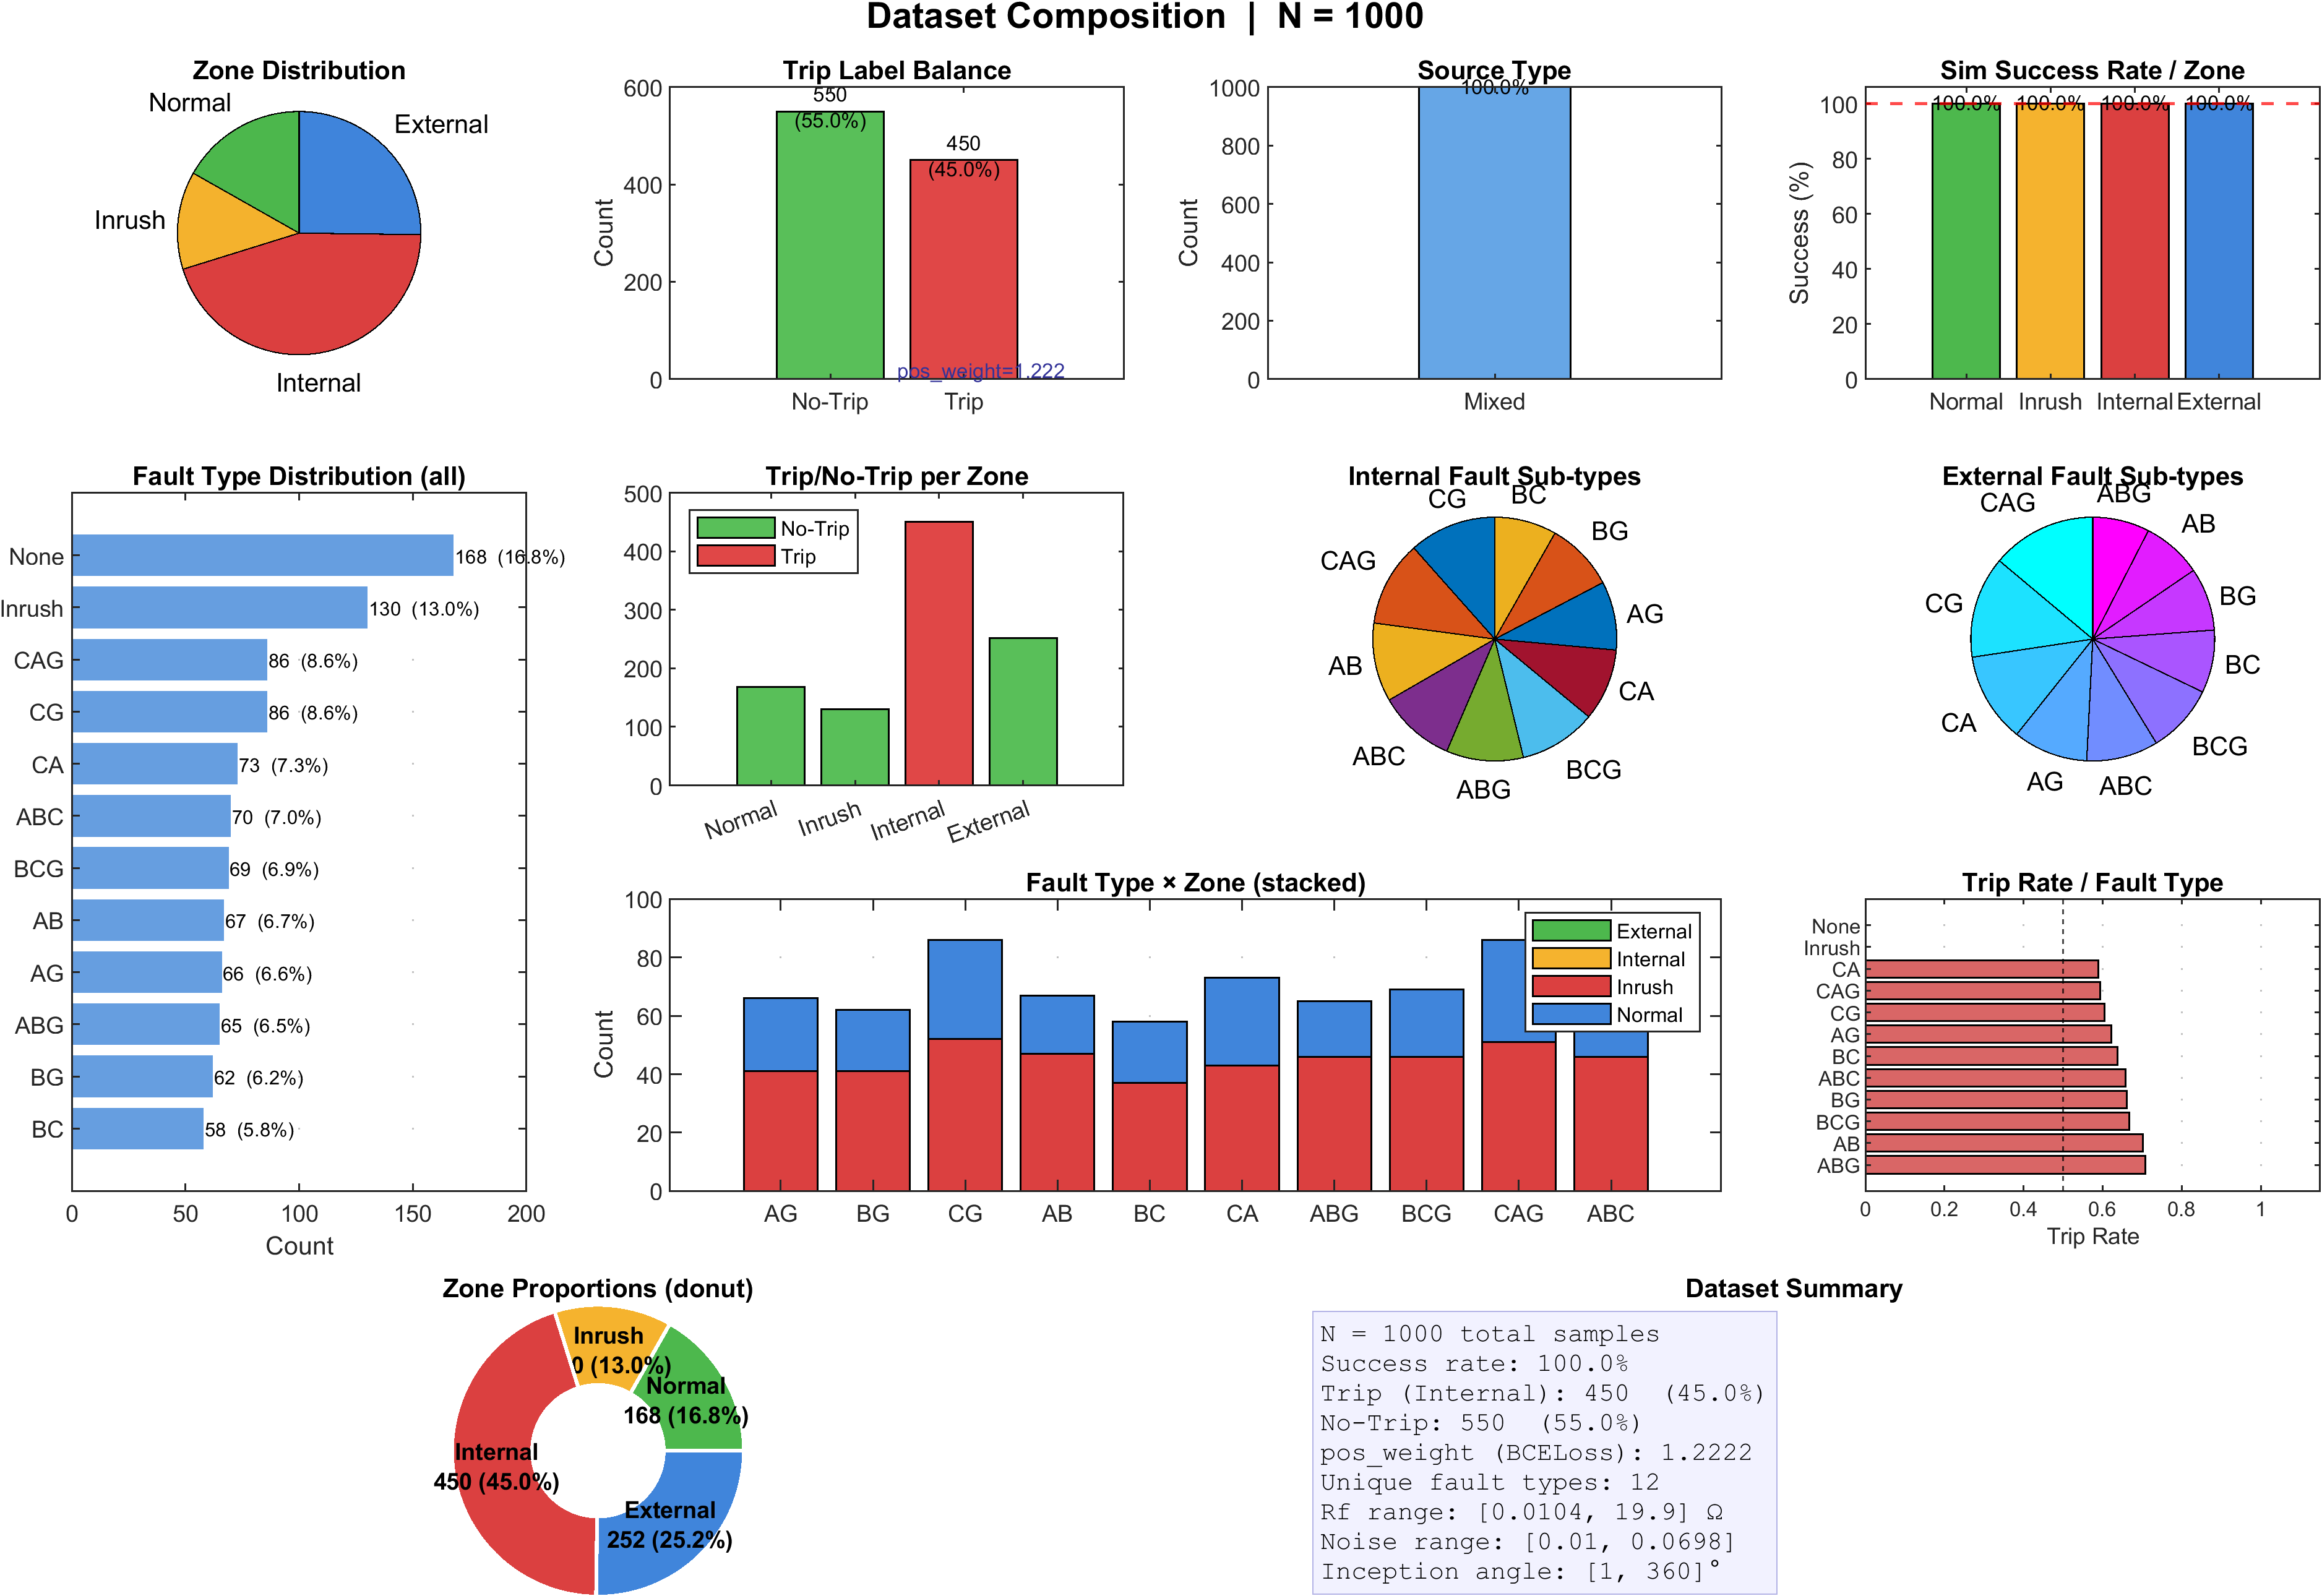
\includegraphics[width=0.7\textwidth]{fig_4_3.png}
\caption{Composition of the 2{,}500-case dataset across event categories and train/validation/test subsets.}\label{fig:4.3}\end{figure}

\chapter{Proposed DWT--LSTM Methodology}
\section{Introduction}
This chapter presents the hybrid adaptive DWT--LSTM framework, which combines MATLAB/Simulink physical modeling and real-time deployment with Python/PyTorch deep-learning training. Differential currents are decomposed by a three-level db4 DWT, yielding two energy features per phase (a compact six-dimensional vector) accumulated over a 32-sample full-cycle buffer. A two-layer LSTM with global temporal attention processes the resulting $[1,32,6]$ tensor; the LSTM acts as a supervisory veto within a hybrid decision engine.

\section{Framework Architecture}
\textbf{Step 1 (MATLAB/Simulink).} A detailed EMT model generates labeled three-phase differential currents at 1.6\,kHz (1601 steps per 1.0\,s), exported to \texttt{.mat}. \textbf{Step 2 (Python/PyTorch).} A DWT engine (PyWavelets) computes approximation and detail energy from 16-sample half-cycle windows; the $[1,32,6]$ tensors train a PyTorch LSTM with global temporal attention using the Adam optimizer and weighted cross-entropy, exported to ONNX at Opset 14 via \texttt{torch.onnx.export}. \textbf{Step 2b (Simulink).} The ONNX model is loaded via the Deep Learning Toolbox Predict block for real-time inference feeding the hybrid decision engine.
\begin{figure}[H]\centering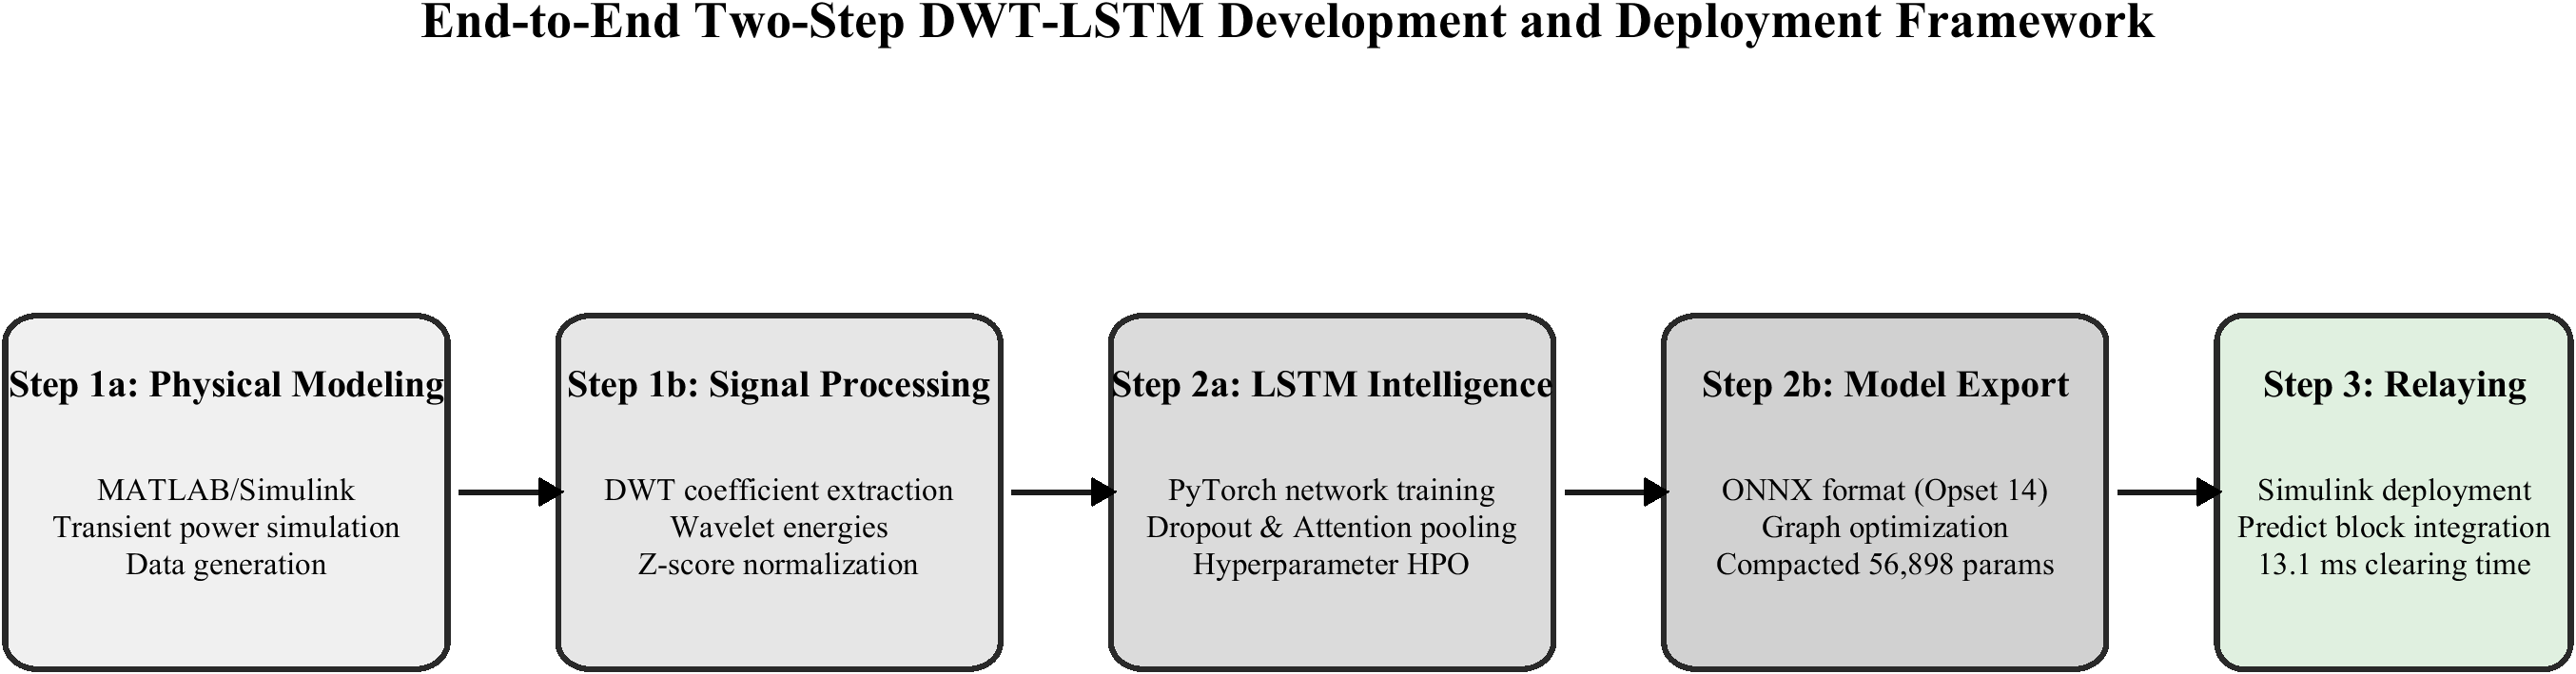
\includegraphics[width=0.95\textwidth]{fig_5_1.png}
\caption{Two-step development and deployment architecture (MATLAB/Simulink $\leftrightarrow$ PyTorch $\leftrightarrow$ ONNX).}\label{fig:5.1}\end{figure}

\subsection{The Hybrid Decision Handshake}
The LSTM operates as a supervisory veto rather than a replacement for the classical relay. The handshake implements a logical AND:
\begin{equation}
\text{TRIP}=\text{Adaptive\_87T}\ \wedge\ (\hat{c}=\text{Internal Fault})\ \wedge\ (\text{Conf}\ge\theta_{conf}),
\end{equation}
providing dependability preservation (the 87T retains primary detection), security enhancement (the LSTM vetoes false trips), and fail-safe operation (defaulting to the 87T on inference failure).
\begin{figure}[H]\centering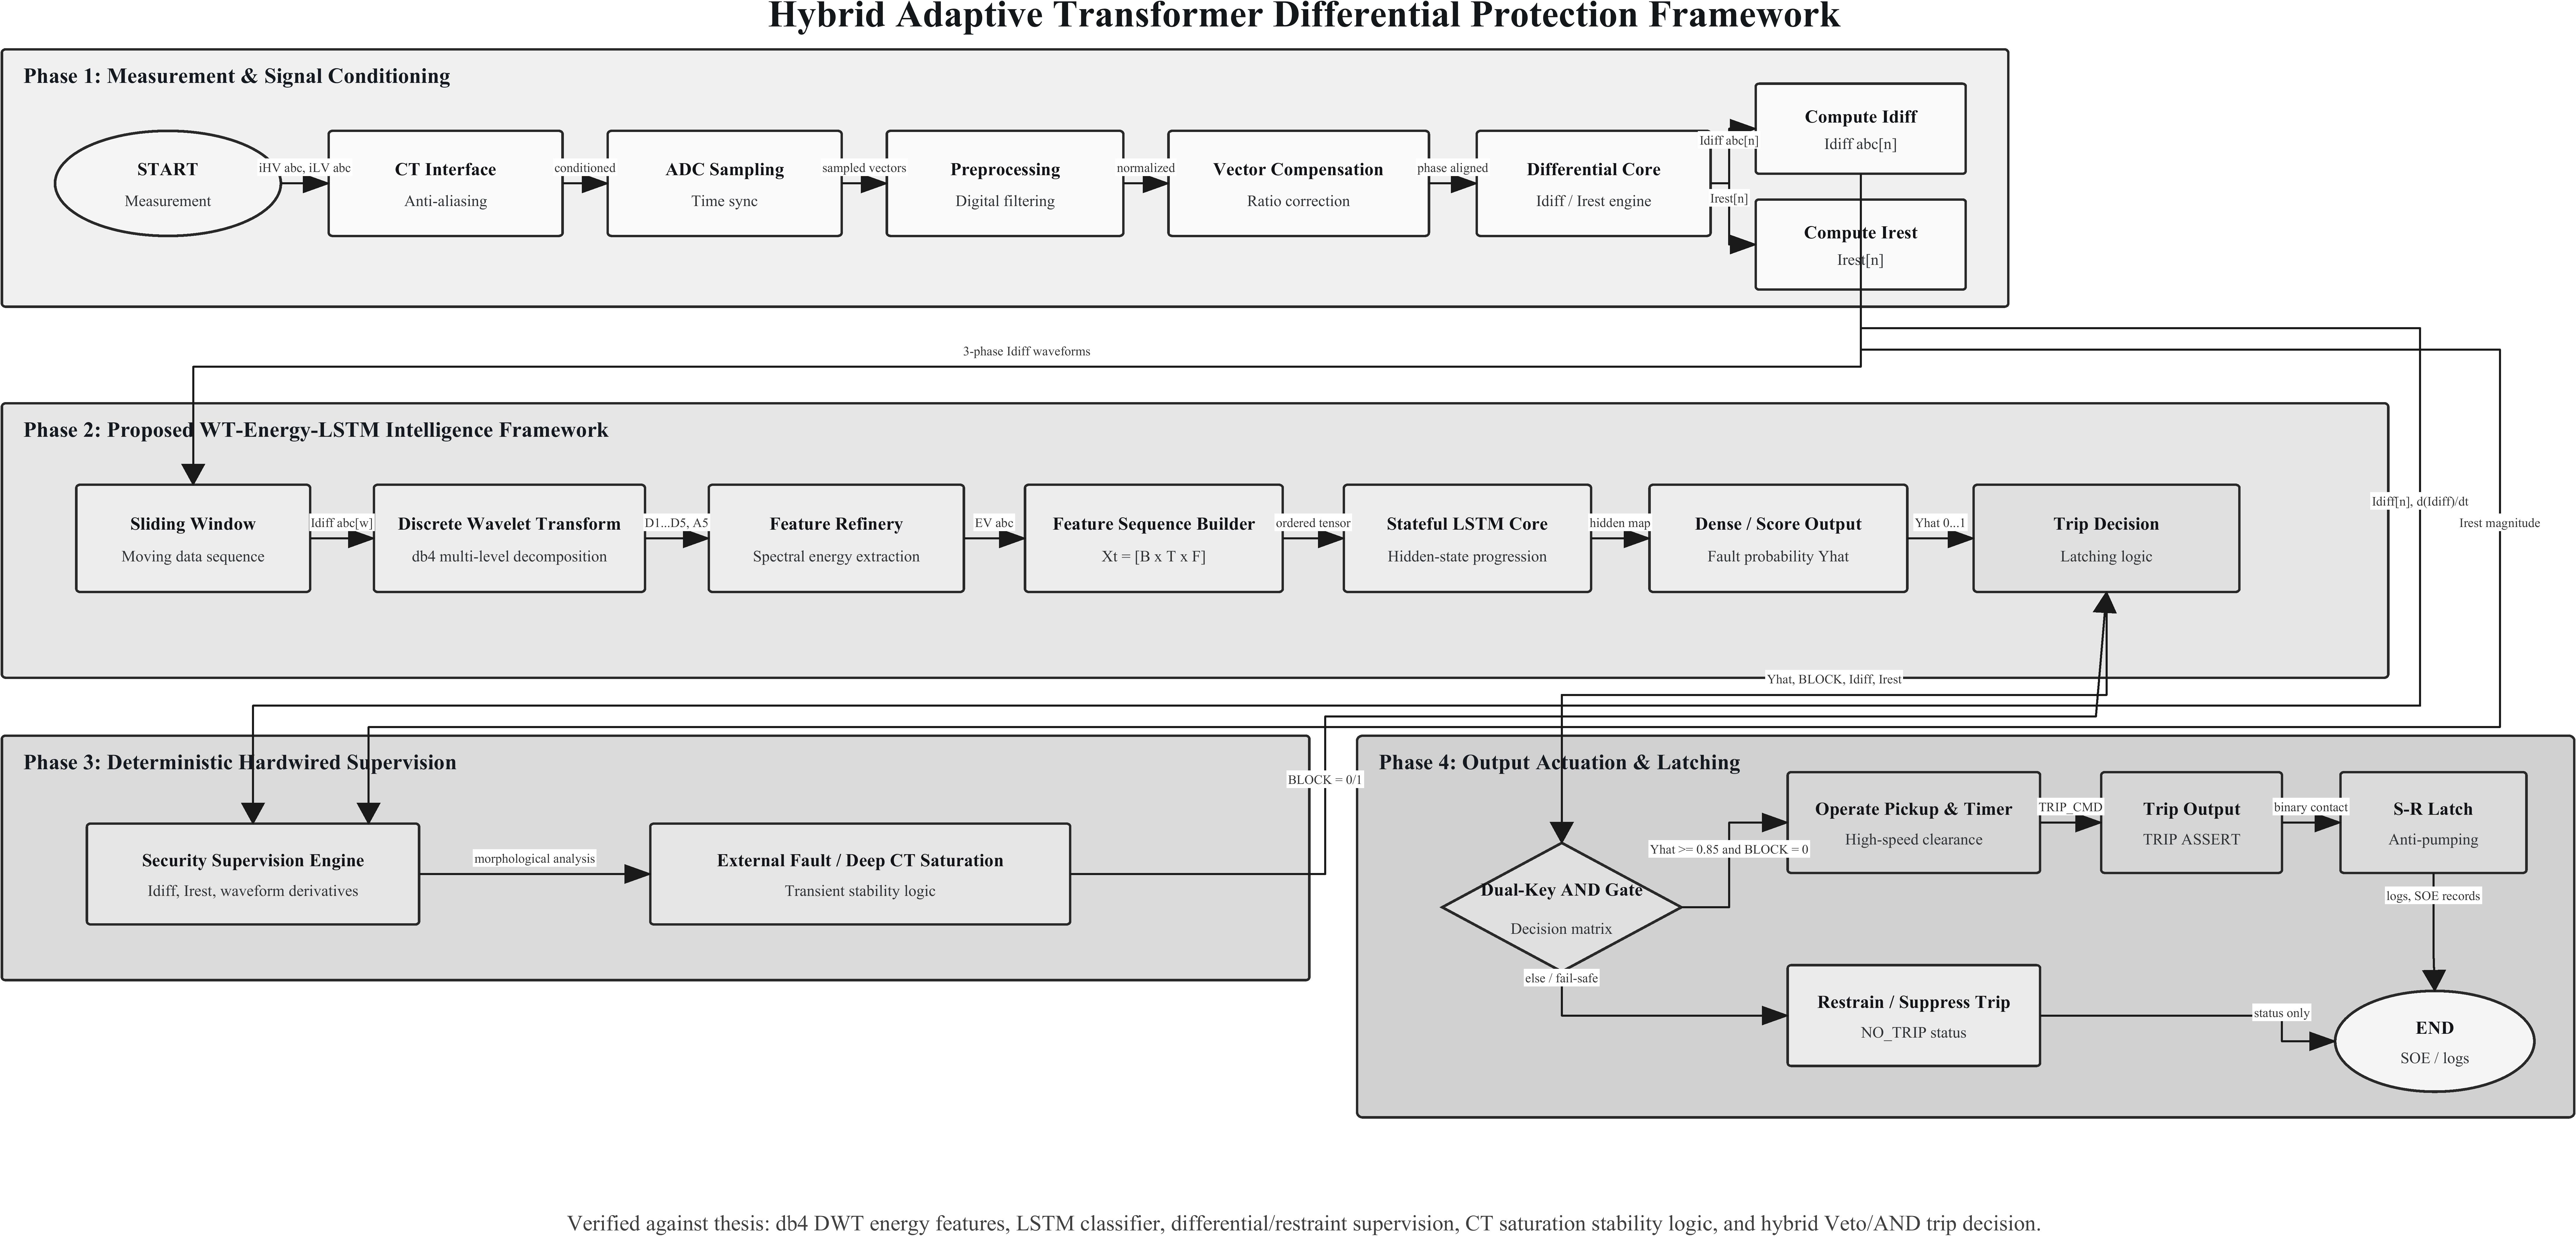
\includegraphics[width=0.95\textwidth]{fig_5_2.png}
\caption{Hybrid veto/AND-gate decision logic combining the adaptive 87T element and the LSTM classifier.}\label{fig:5.2}\end{figure}

\subsection{Signal Flow}
The pipeline comprises seven stages: (1) CT secondary and merging unit at 1.6\,kHz with Yd1 ($-30^\circ$) compensation; (2) 16-sample half-cycle window; (3) 3-level db4 DWT yielding the six-element energy vector; (4) 32-sample full-cycle buffer reshaped to $[1,32,6]$; (5) ONNX LSTM classification; (6) hybrid decision engine; (7) latched breaker trip.
\begin{figure}[H]\centering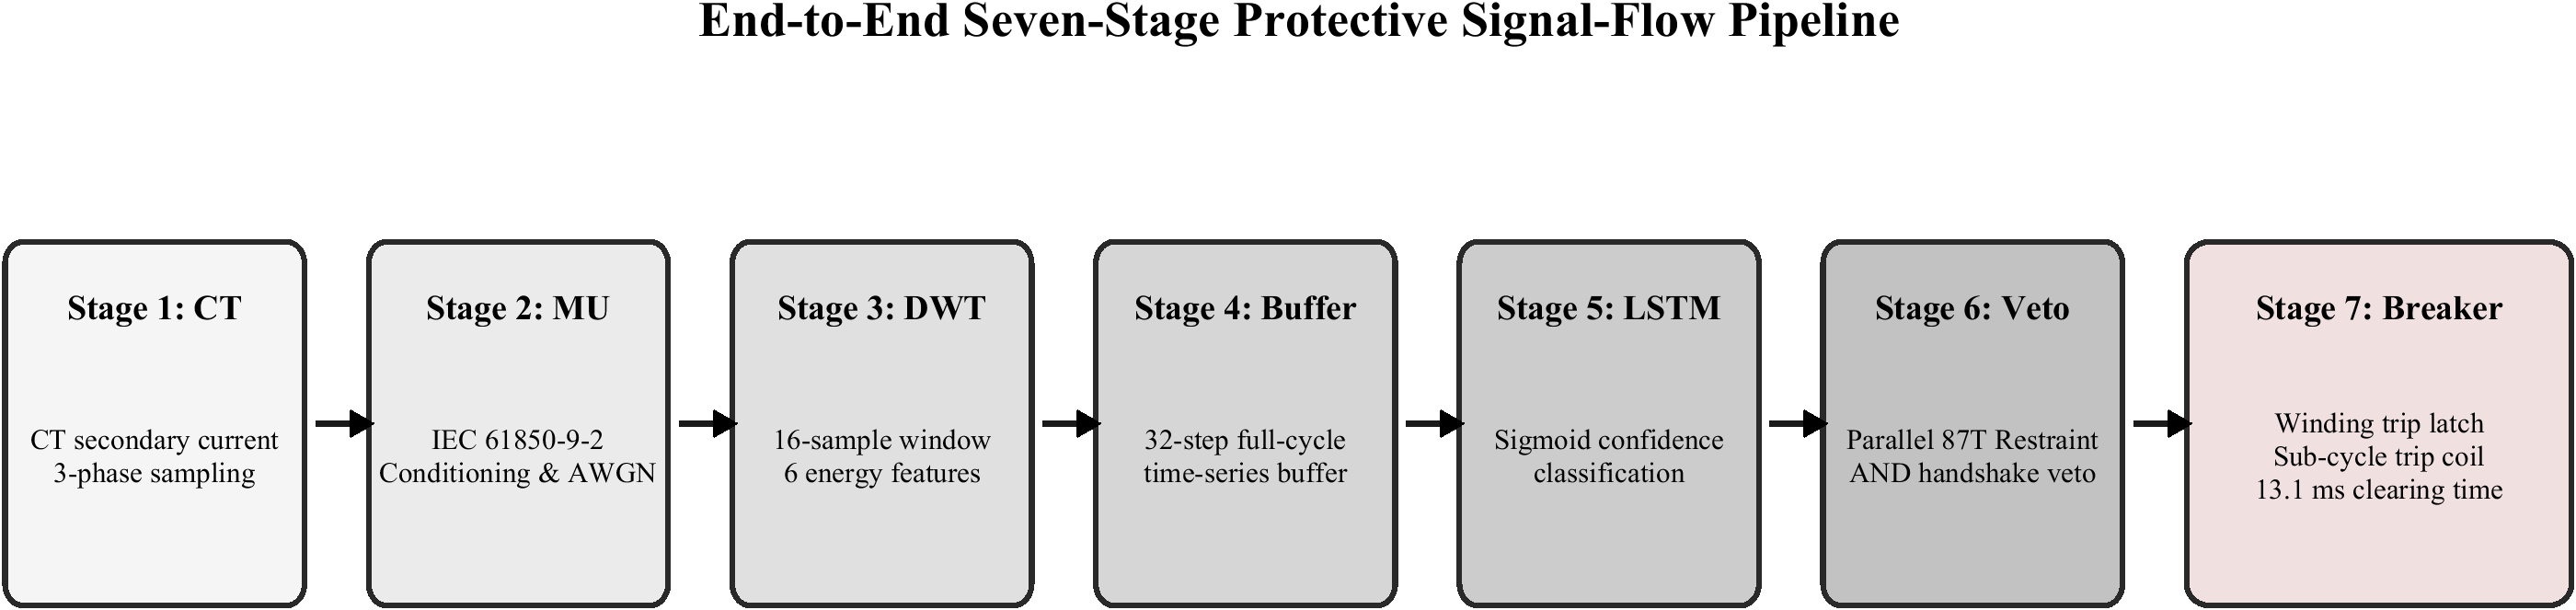
\includegraphics[width=0.95\textwidth]{fig_5_3.png}
\caption{End-to-end seven-stage signal flow of the proposed protection scheme.}\label{fig:5.3}\end{figure}

\section{Data Preprocessing and Sampling}
The framework adopts $f_s=N\!\times\!f_0=32\times50=1600$\,Hz ($\Delta t=0.625$\,ms), satisfying Nyquist for components up to the 10th harmonic and enabling clean dyadic decomposition of the 16-sample window ($16\!\to\!8\!\to\!4\!\to\!2$). Two sliding windows operate at different scales: a 16-sample (10\,ms) half-cycle DWT window and a 32-sample (20\,ms) full-cycle LSTM buffer.
\begin{figure}[H]\centering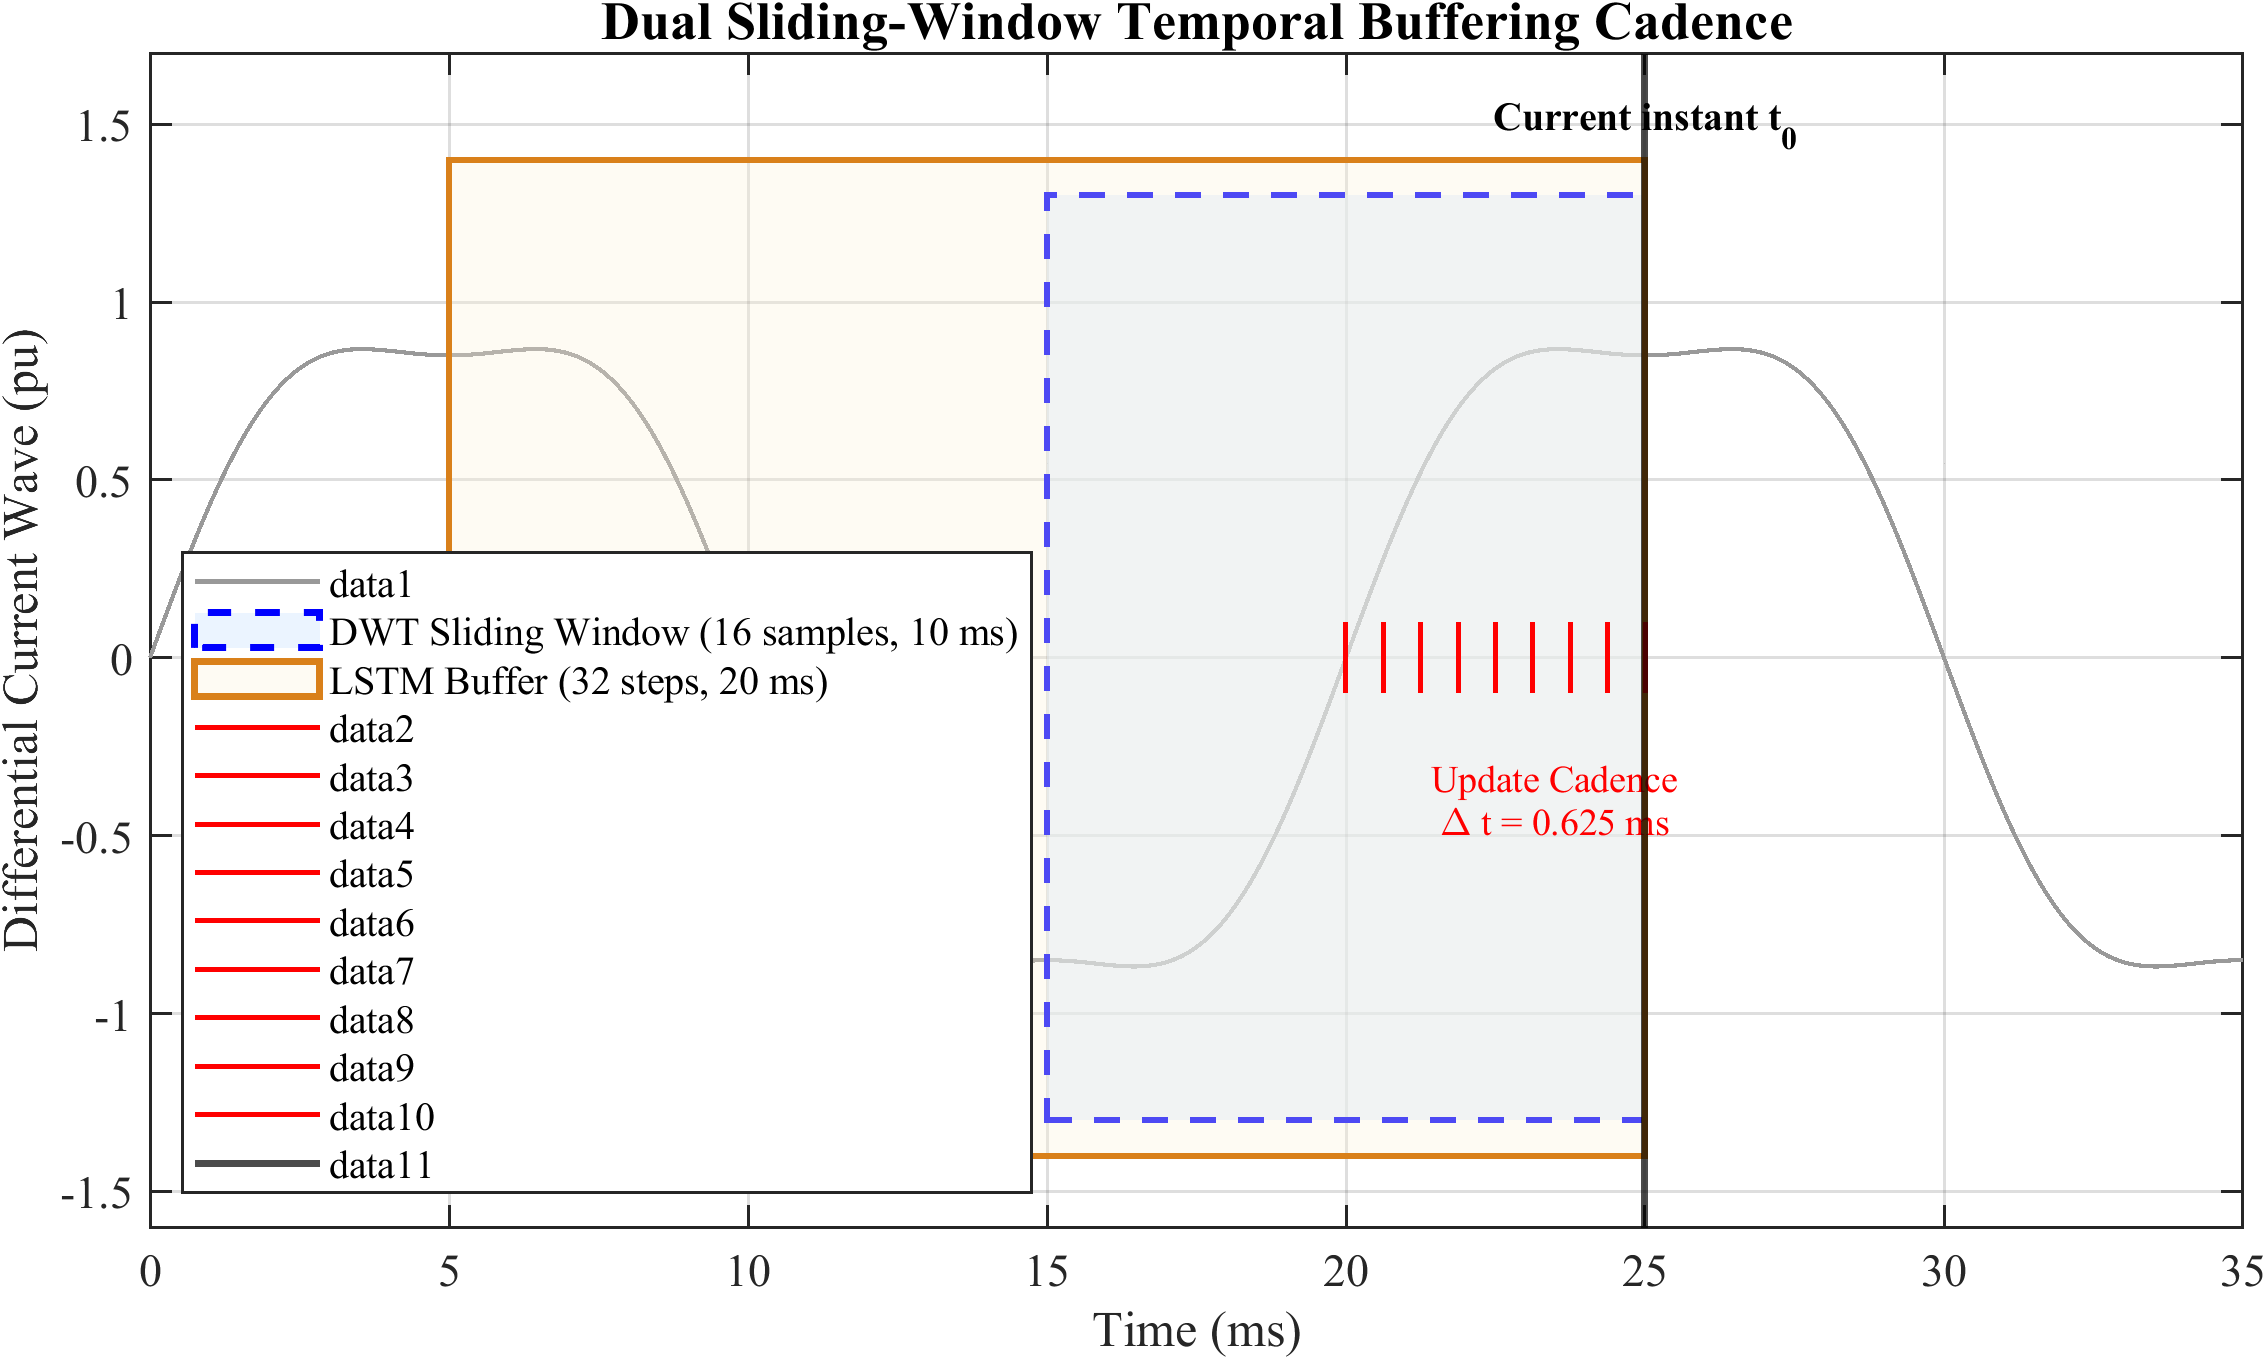
\includegraphics[width=0.8\textwidth]{fig_5_4.png}
\caption{Dual sliding-window timing: half-cycle DWT window and full-cycle LSTM buffer.}\label{fig:5.4}\end{figure}

\section{DWT Engine and Feature Extraction}
The db4 wavelet (compact support $L=8$, four vanishing moments, orthogonal) matches fault-inception transients. The 3-level decomposition follows the Mallat algorithm with quadrature mirror filters $h[n]$ and $g[n]=(-1)^n h[L-1-n]$ and downsampling:
\begin{equation}
a_j[k]=\sum_n h[n-2k]\,a_{j-1}[n],\qquad d_j[k]=\sum_n g[n-2k]\,a_{j-1}[n].
\end{equation}
The band allocation is given in Table~\ref{tab:5.2}. Two energy features per phase follow from Parseval's theorem: the approximation energy $E_{A,\varphi}=\sum_k|a_3^{(\varphi)}[k]|^2$ (0--100\,Hz) and the detail energy $E_{D,\varphi}=\sum_{j=1}^{3}\sum_k|d_j^{(\varphi)}[k]|^2$ (100--800\,Hz).
\begin{table}[H]\centering\caption{Frequency band allocation for the 3-level DWT at 1.6\,kHz.}\label{tab:5.2}
\begin{tabular}{@{}ccll c@{}}\toprule \textbf{Level} & \textbf{Coeff.} & \textbf{Band (Hz)} & \textbf{Key components} & \textbf{\# Coeff.}\\ \midrule
3 & $a_3$ & 0--100 & DC, fundamental (50\,Hz) & 2\\
3 & $d_3$ & 100--200 & 2nd--4th harmonics & 2\\
2 & $d_2$ & 200--400 & 4th--8th harmonics & 4\\
1 & $d_1$ & 400--800 & High-freq.\ transients & 8\\ \bottomrule
\end{tabular}\end{table}
The six-dimensional feature vector $f(t)=[E_{A,A},E_{D,A},E_{A,B},E_{D,B},E_{A,C},E_{D,C}]$ is $z$-score normalized and accumulated over the full-cycle buffer into $X(t)\in\mathbb{R}^{32\times6}$, reshaped to $X_{LSTM}\in\mathbb{R}^{1\times32\times6}$.
\begin{figure}[H]\centering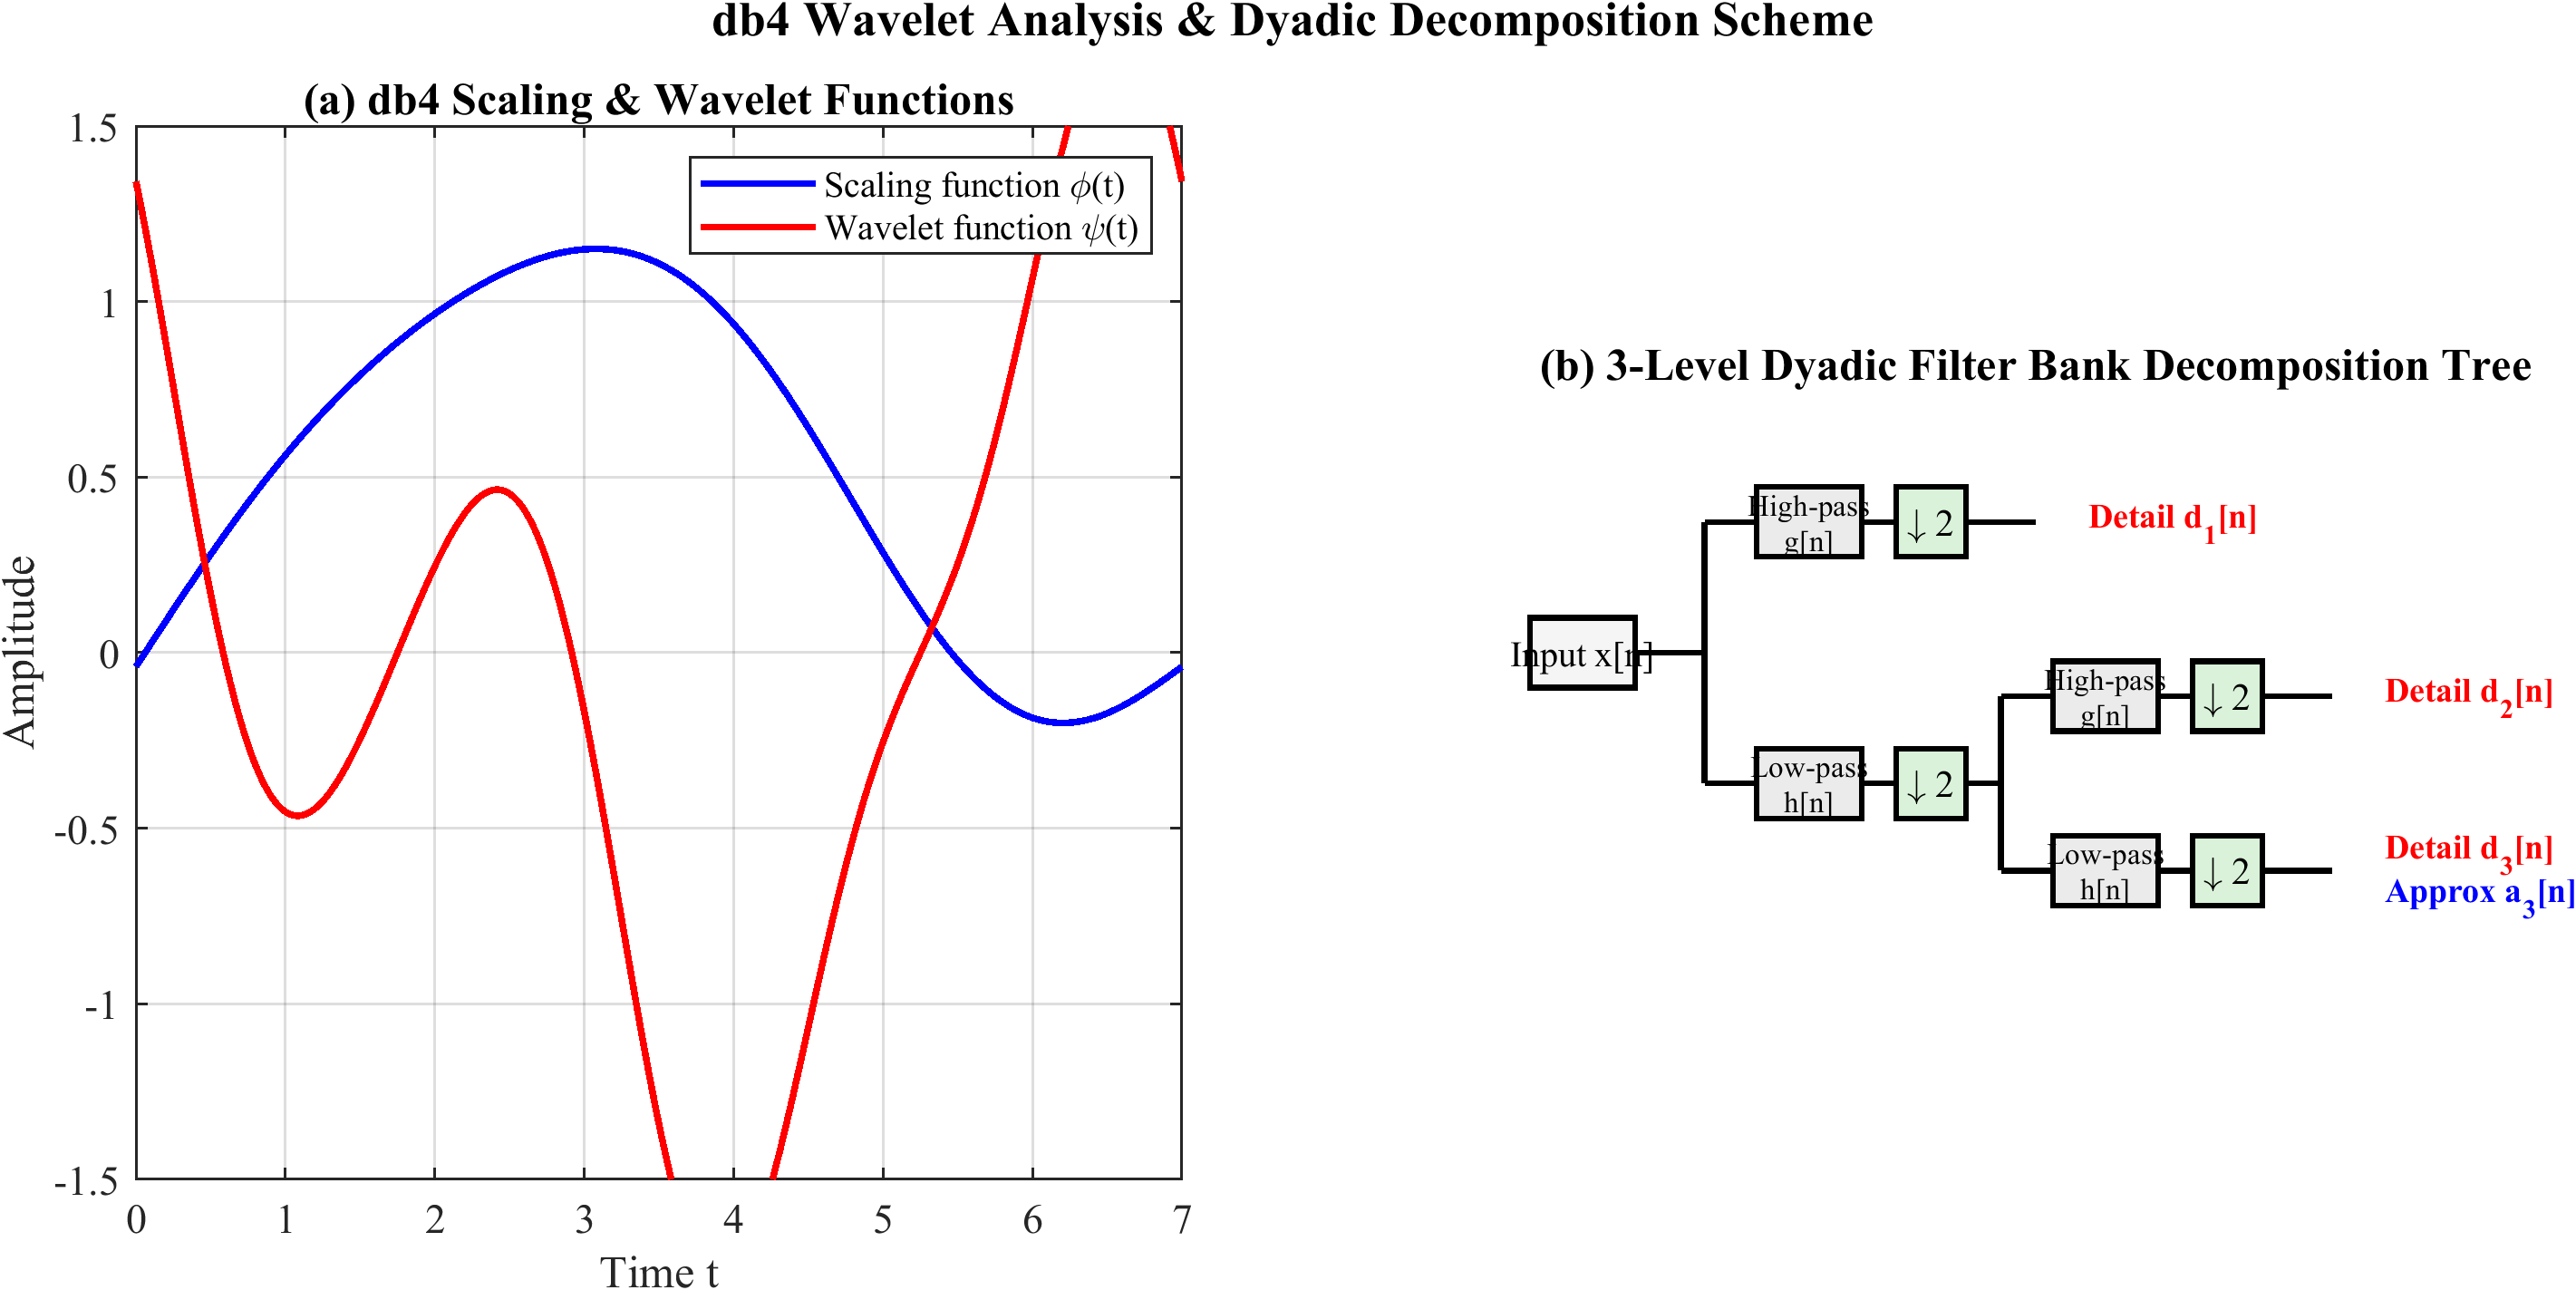
\includegraphics[width=0.85\textwidth]{fig_5_5.png}
\caption{db4 mother wavelet and the three-level dyadic filter-bank decomposition tree.}\label{fig:5.5}\end{figure}

\section{LSTM Architecture and Training}
The network comprises an input layer $[B,32,6]$; LSTM-1 (128 units, return sequences) with dropout 0.3; LSTM-2 (64 units, return sequences) with dropout 0.3; a global temporal attention layer
\begin{equation}
\alpha_t=\frac{\exp(v^\top\tanh(W_a h_t+b_a))}{\sum_{t'=1}^{32}\exp(v^\top\tanh(W_a h_{t'}+b_a))},\qquad c=\sum_{t=1}^{32}\alpha_t h_t\in\mathbb{R}^{64};
\end{equation}
a dense layer (32 units, ReLU); and a softmax output. The total trainable parameter count is 125{,}476.
\begin{figure}[H]\centering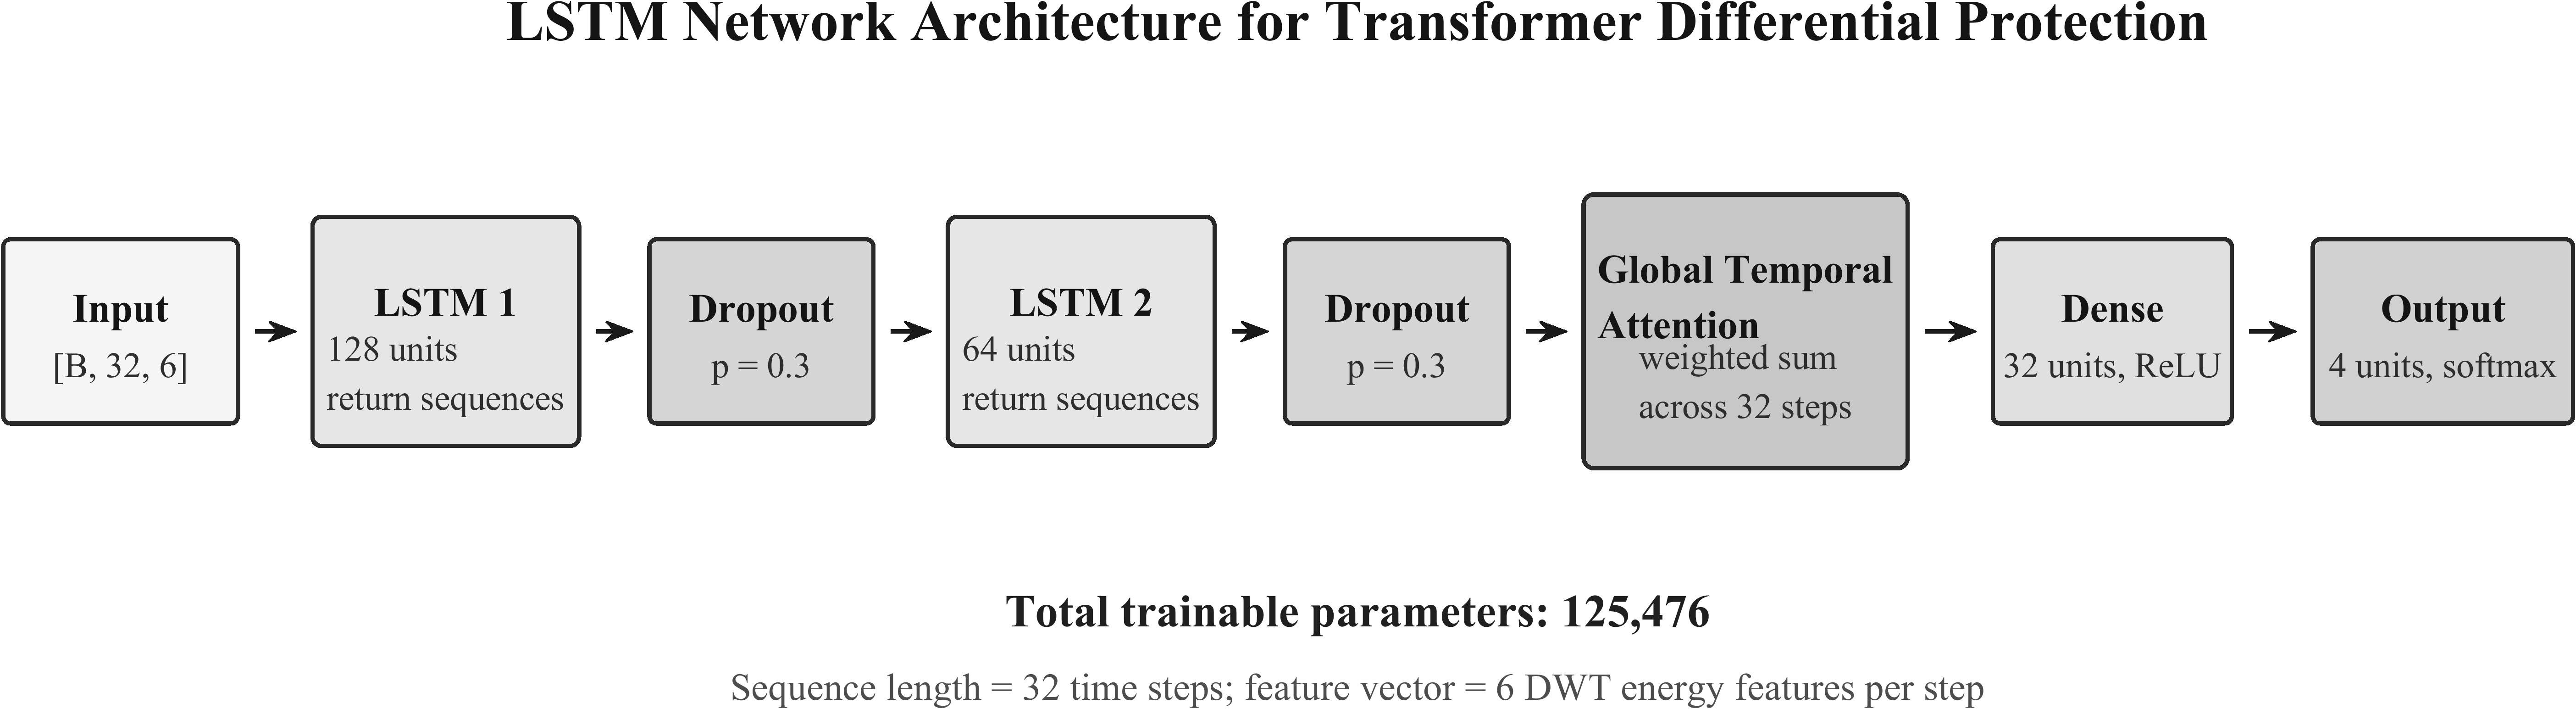
\includegraphics[width=0.95\textwidth]{fig_5_6.png}
\caption{DWT--LSTM classifier architecture with global temporal attention.}\label{fig:5.6}\end{figure}
Training uses weighted cross-entropy (positive-class weight 1.4155), Adam ($\eta=0.001$, $\beta_1=0.9$, $\beta_2=0.999$), a ReduceLROnPlateau scheduler, batch size 128, up to 200 epochs with early stopping (patience 20), and 5-fold stratified cross-validation. The confidence score is $\text{Conf}(t)=\max_c\hat{p}_c(t)$ with $\theta_{conf}=0.85$. The model is exported to ONNX (Opset 14) with a fixed $[1,32,6]$ input and a stateless graph.

\section{Real-Time Implementation and Latency}
The ONNX model is integrated via the Predict block within a masked subsystem; a Stateflow chart encodes the trip/block state machine and latches the trip for 100\,ms. The processing latency is $T_{proc}=T_{buffer}+T_{DWT}+T_{LSTM}+T_{logic}\approx5.0+0.1+1.0+0.01=6.1$\,ms ($\approx$0.3 cycle); the LSTM contributes 0.5--2.0\,ms on CPU ($<$0.1\,ms on GPU), with a total cost of $\approx$1.31\,MFLOPs per step.
\begin{table}[H]\centering\caption{Per-inference parameter and operation budget of the DWT--LSTM pipeline.}\label{tab:5.3}
\begin{tabular}{@{}lccc@{}}\toprule \textbf{Stage} & \textbf{Parameters} & \textbf{FLOPs/step} & \textbf{Share (\%)}\\ \midrule
DWT (3-level db4, $\times3$) & 0 & $\approx$3.1\,k & 0.2\\
LSTM layer 1 ($6\!\to\!128$) & 69{,}632 & $\approx$0.55\,M & 42.0\\
LSTM layer 2 ($128\!\to\!64$) & 49{,}408 & $\approx$0.69\,M & 52.7\\
Attention (64) & 4{,}224 & $\approx$0.06\,M & 4.6\\
Dense + softmax & 2{,}212 & $\approx$6.5\,k & 0.5\\ \midrule
Total & 125{,}476 & $\approx$1.31\,M & 100\\ \bottomrule
\end{tabular}\end{table}
\begin{figure}[H]\centering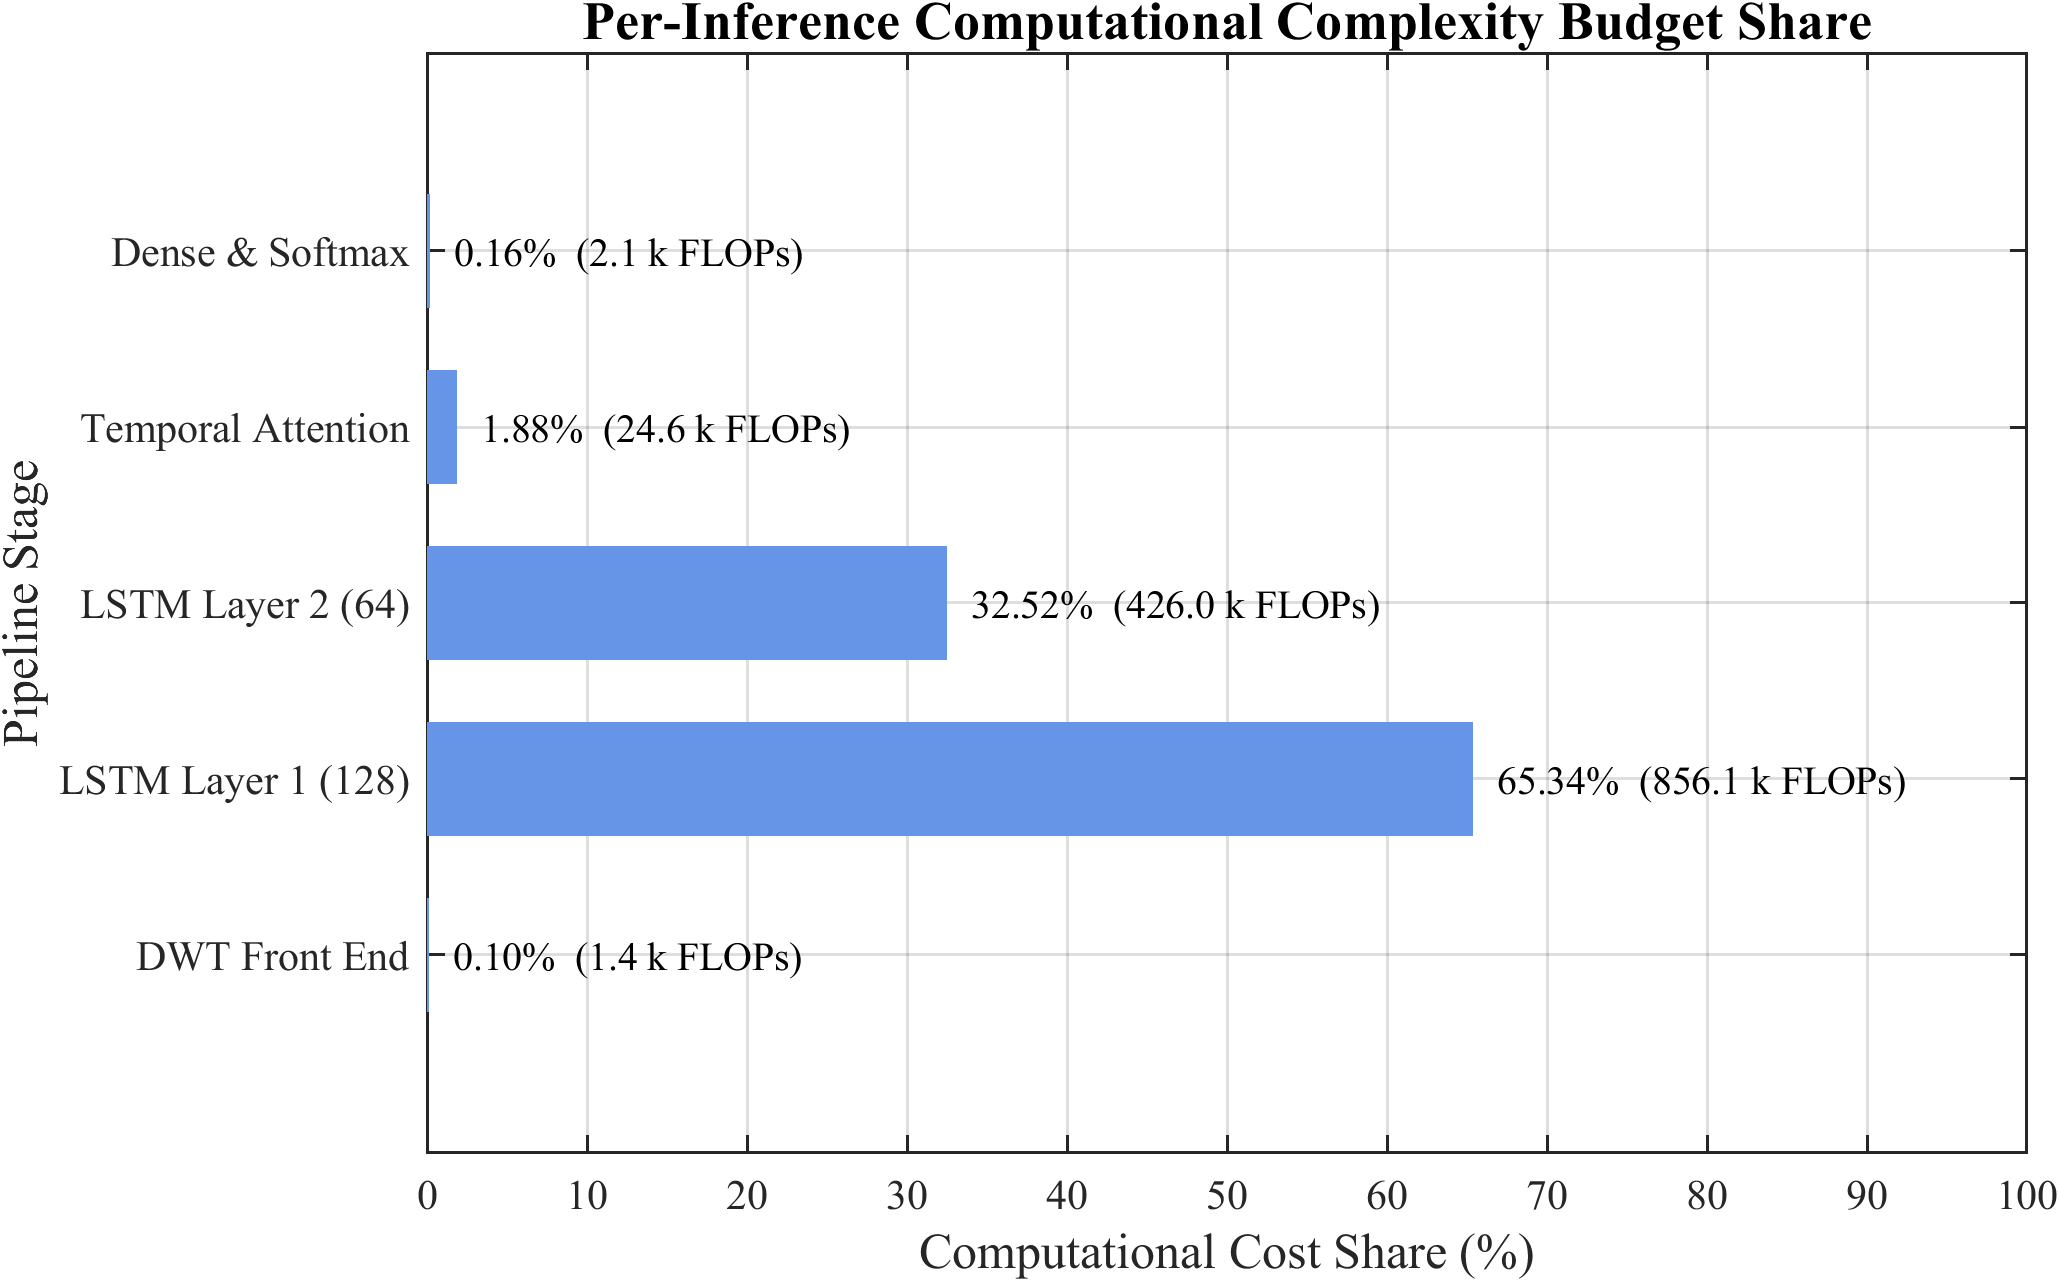
\includegraphics[width=0.7\textwidth]{fig_5_7.png}
\caption{Per-inference computational cost distribution across pipeline stages.}\label{fig:5.7}\end{figure}

\section{Robustness Enhancement}
Three complementary strategies are used: AWGN augmentation (20/30/40\,dB, with 15/50\,dB for stress) exploiting the inherent noise resilience of frequency-localized energy features; dropout regularization (0.3) between LSTM layers; and out-of-distribution stress testing across switching angle, frequency (47--53\,Hz), remanent flux ($\pm0.9 B_{sat}$), and CT ratio errors ($\pm5\%$), processed end-to-end through the Simulink-embedded ONNX model.

\chapter{Results, Analysis and Discussion}
\section{Introduction}
This chapter evaluates the proposed Hybrid Adaptive Transformer Differential Protection (HATDP) framework, in which a DWT--LSTM classifier supervises a conventional 87T relay. All data were generated for a 300\,MVA, 230/11\,kV, Yd1 transformer at 1.6\,kHz. A dataset of 2{,}500 base cases (Table~\ref{tab:4.3}) was augmented and split 70/15/15, yielding an 1{,}800-case held-out test set. For protection evaluation the four categories are mapped to a binary decision (Trip vs.\ No-Trip).

\section{Data Generation and Preprocessing}
Figure~\ref{fig:6.1} shows representative three-phase differential current waveforms: normal load below 0.02\,pu; external faults decaying within one cycle; inrush with 5--8\,pu asymmetric peaks; and internal faults with sustained high-magnitude, high-frequency content. Severe CT saturation produced 34.7\% THD and 18.2\% second-harmonic content, consistent with IEEE C37.110.
\begin{figure}[H]\centering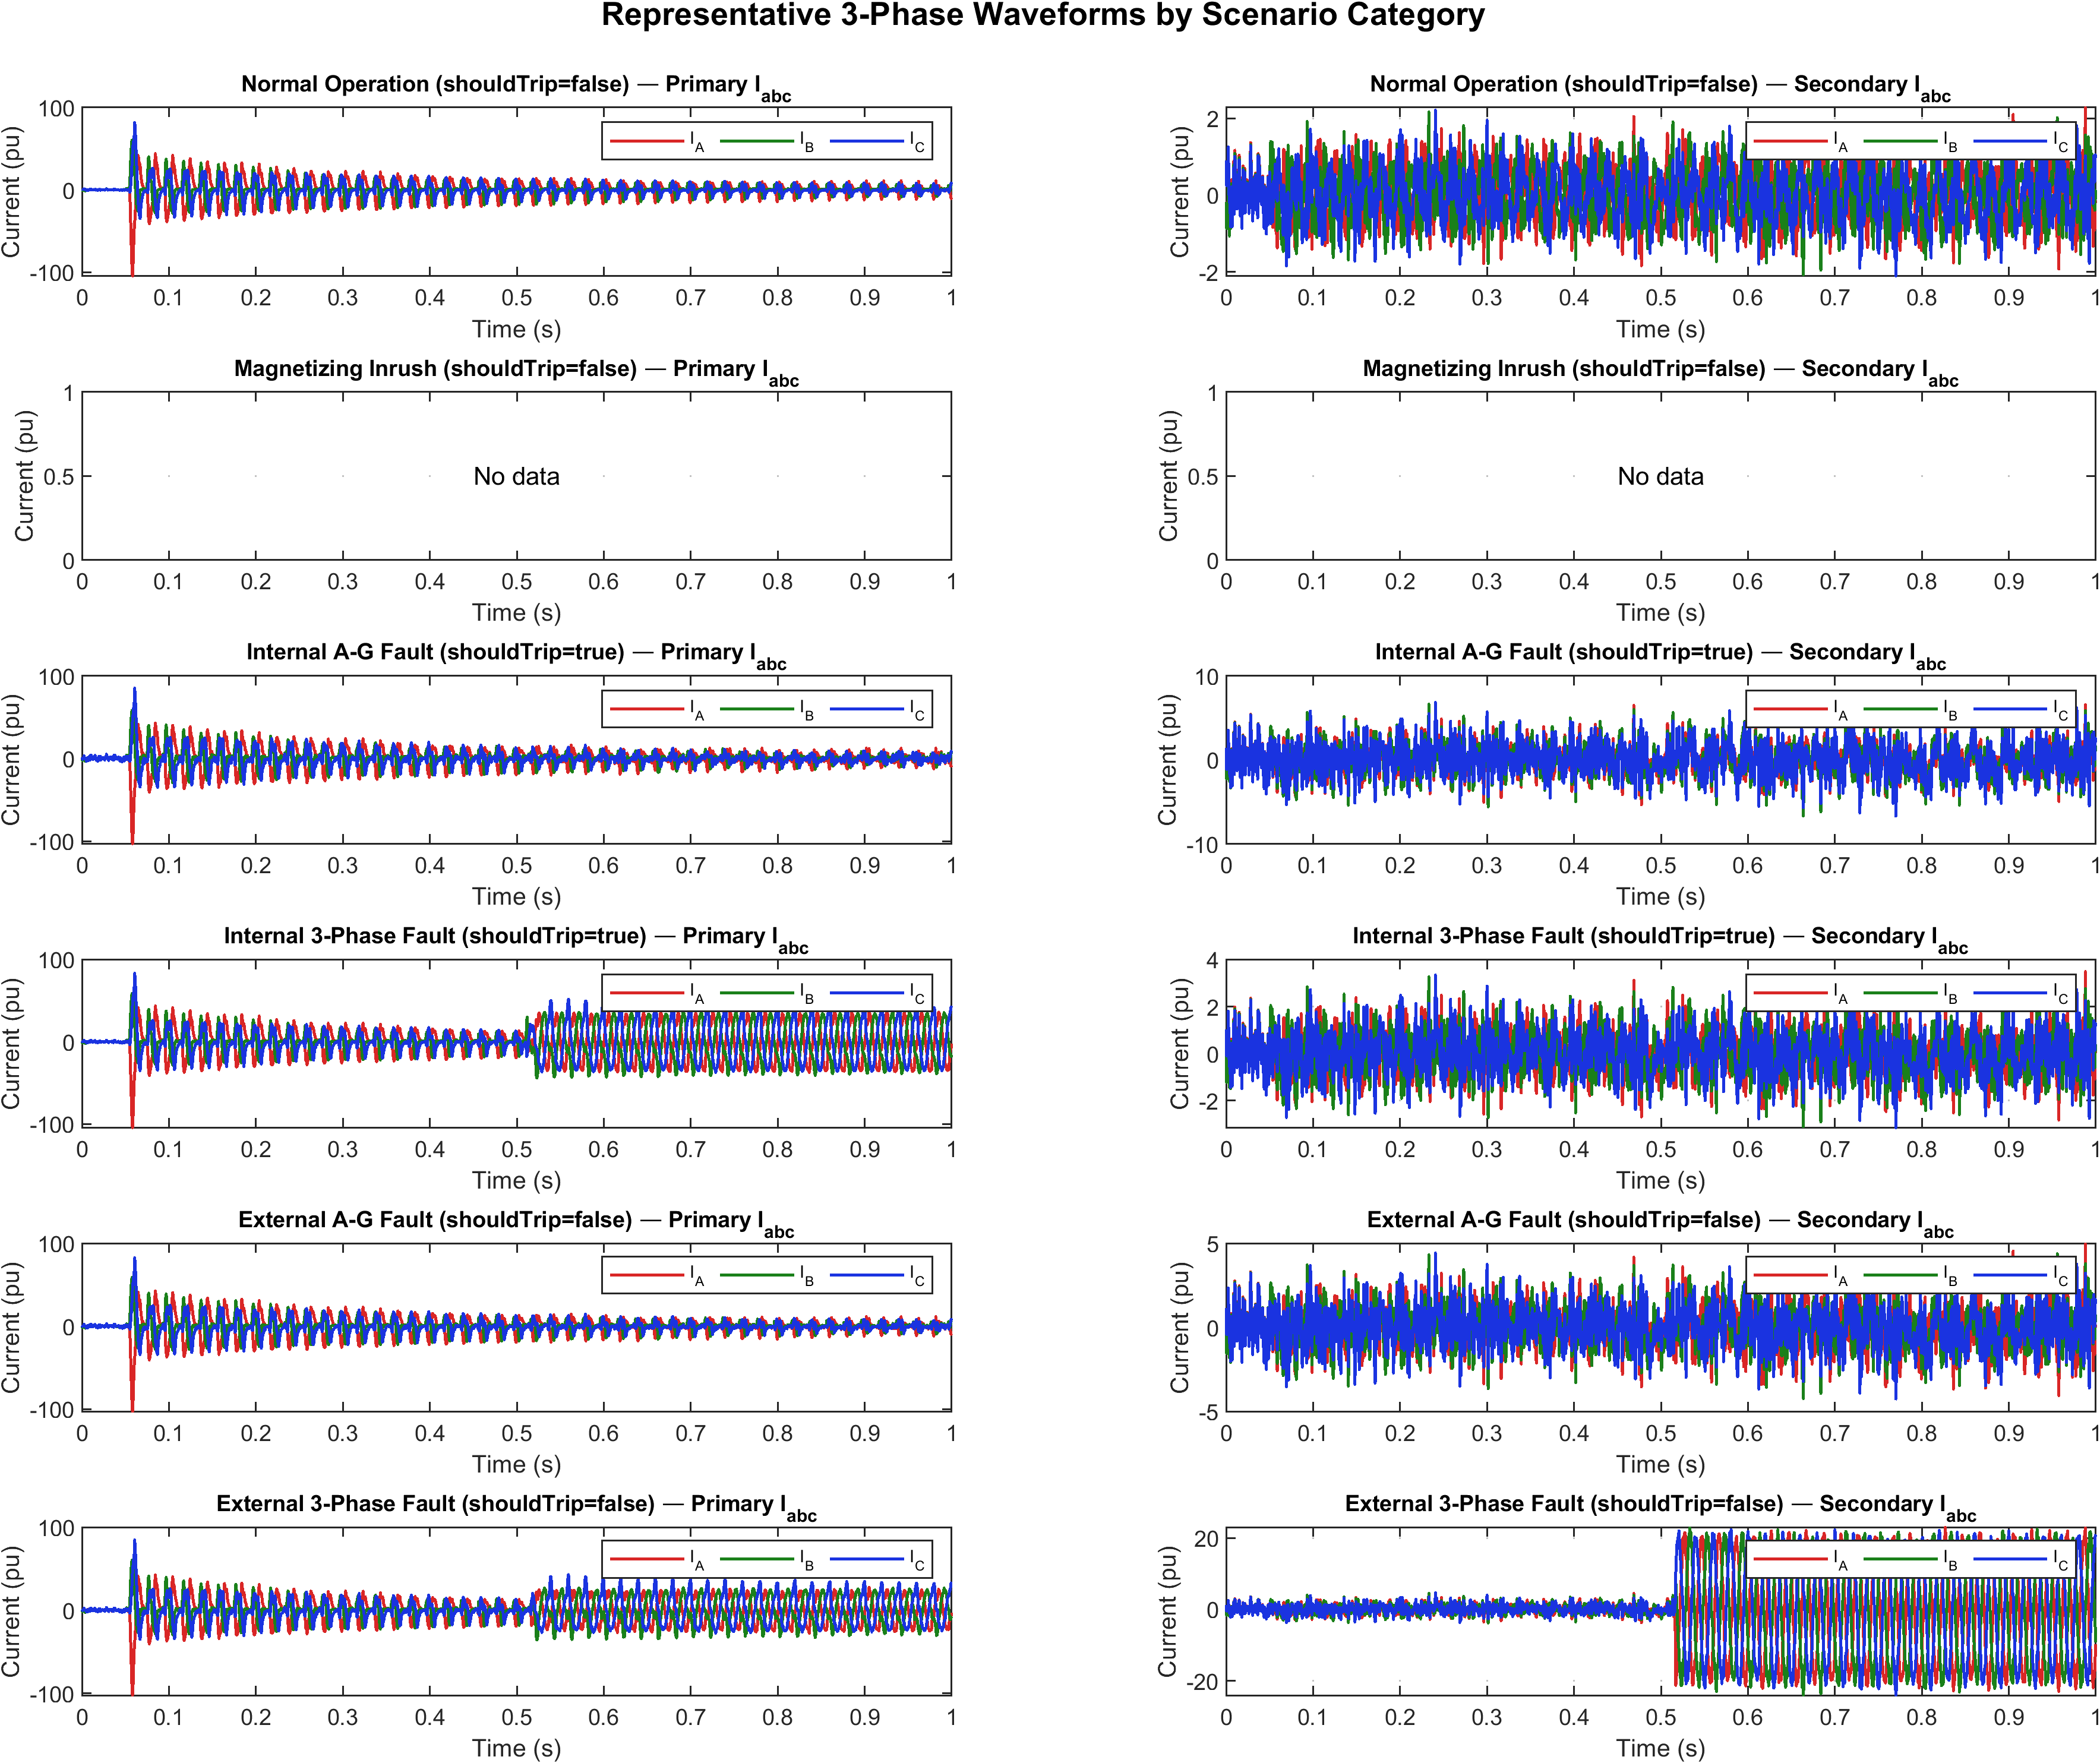
\includegraphics[width=0.55\textwidth]{fig_6_1.png}
\caption{Three-phase differential current waveforms for the four operating conditions.}\label{fig:6.1}\end{figure}
The six energy features---approximation energy $E_A$ (0--100\,Hz) and detail energy $E_D$ (100--800\,Hz) per phase---separate the classes strongly, the Phase-C detail energy showing an inter-class separation ratio of $502\times$ between internal faults and normal operation (Table~\ref{tab:6.1}). Mutual-information analysis confirms the detail-energy features dominate (72.3\% of total MI); an ablation gives 98.83\% for detail-only, 91.24\% for approximation-only, and 98.89\% for the full set.
\begin{table}[H]\centering\caption{Statistical distribution of the six DWT energy features across event classes (mean $\pm$ s.d., $\times10^{-3}$\,pu$^2$).}\label{tab:6.1}
\small\begin{tabular}{@{}lcccc@{}}\toprule \textbf{Feature} & \textbf{Normal} & \textbf{External} & \textbf{Inrush} & \textbf{Internal}\\ \midrule
$E_A$ -- Phase A & $0.08\pm0.03$ & $0.42\pm0.18$ & $1.85\pm0.72$ & $3.27\pm1.14$\\
$E_A$ -- Phase B & $0.07\pm0.02$ & $0.39\pm0.16$ & $1.72\pm0.68$ & $3.15\pm1.08$\\
$E_A$ -- Phase C & $0.09\pm0.03$ & $0.44\pm0.19$ & $1.91\pm0.75$ & $3.41\pm1.21$\\
$E_D$ -- Phase A & $0.01\pm0.005$ & $0.15\pm0.08$ & $0.52\pm0.21$ & $4.86\pm1.92$\\
$E_D$ -- Phase B & $0.01\pm0.004$ & $0.13\pm0.07$ & $0.48\pm0.19$ & $4.71\pm1.85$\\
$E_D$ -- Phase C & $0.01\pm0.006$ & $0.16\pm0.09$ & $0.55\pm0.23$ & $5.02\pm2.01$\\ \bottomrule
\end{tabular}\end{table}
\begin{figure}[H]\centering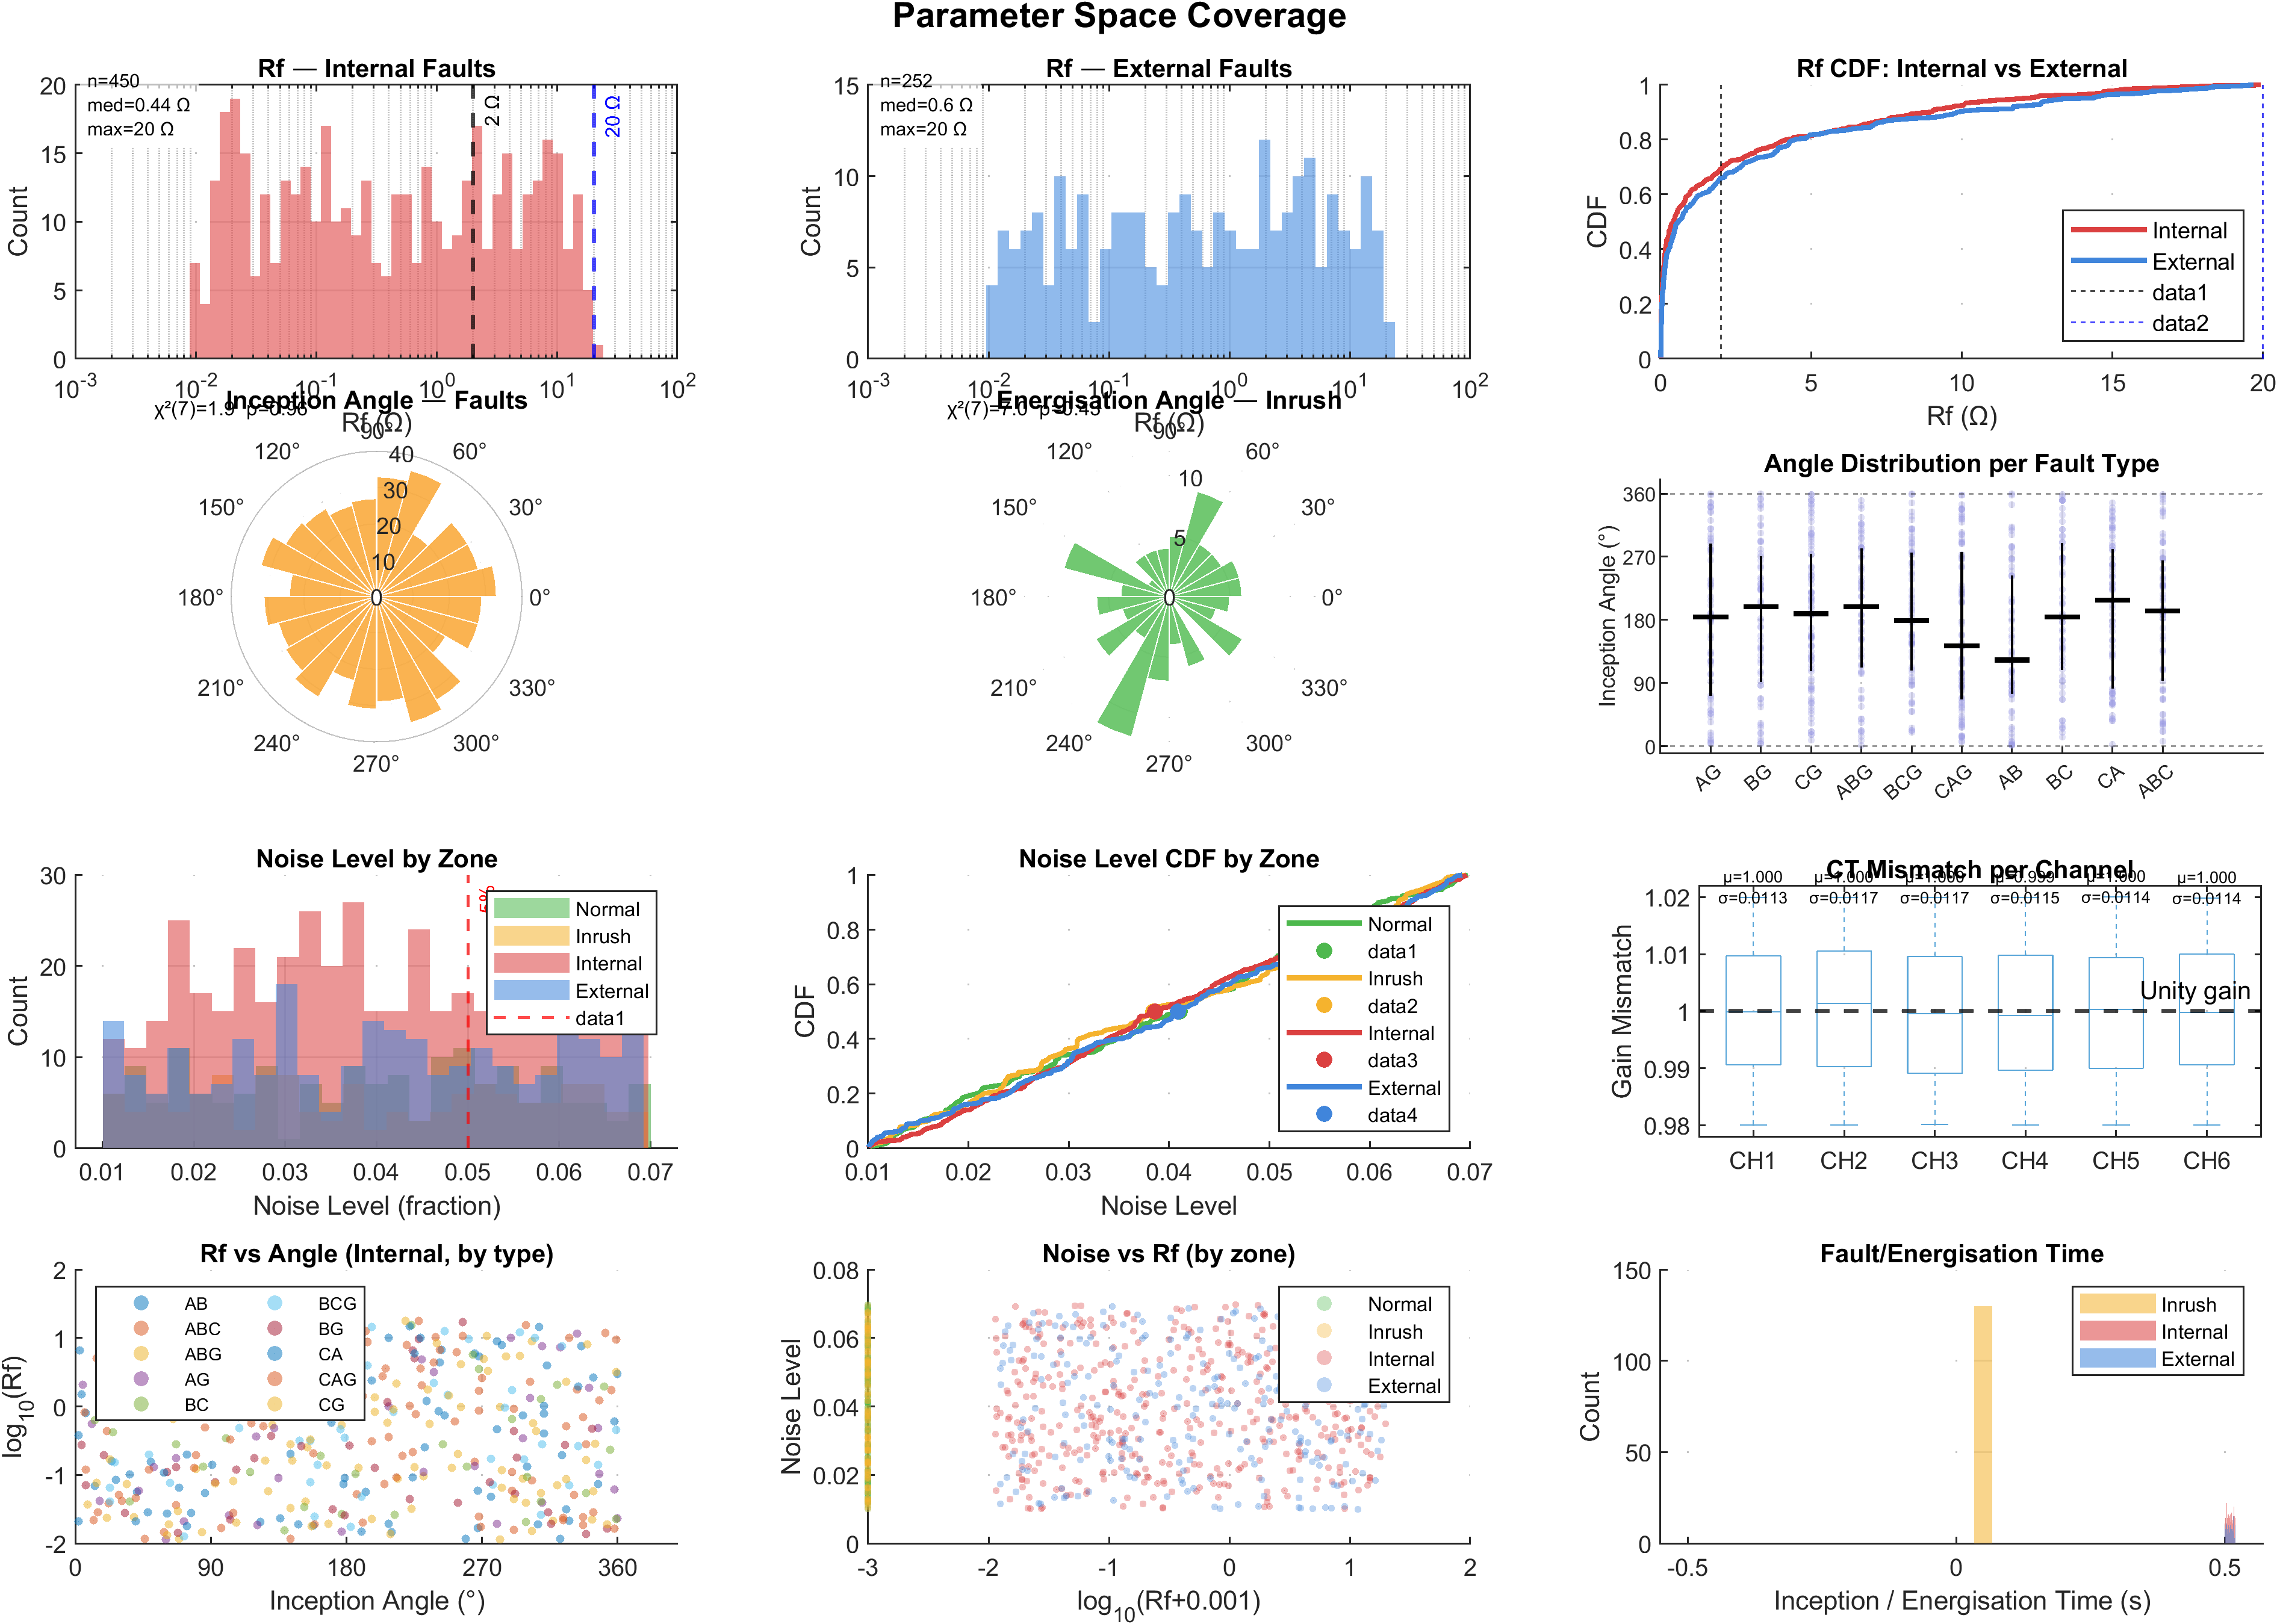
\includegraphics[width=0.62\textwidth]{fig_6_2.png}
\caption{Parameter-space coverage / feature distribution across event classes.}\label{fig:6.2}\end{figure}
\begin{figure}[H]\centering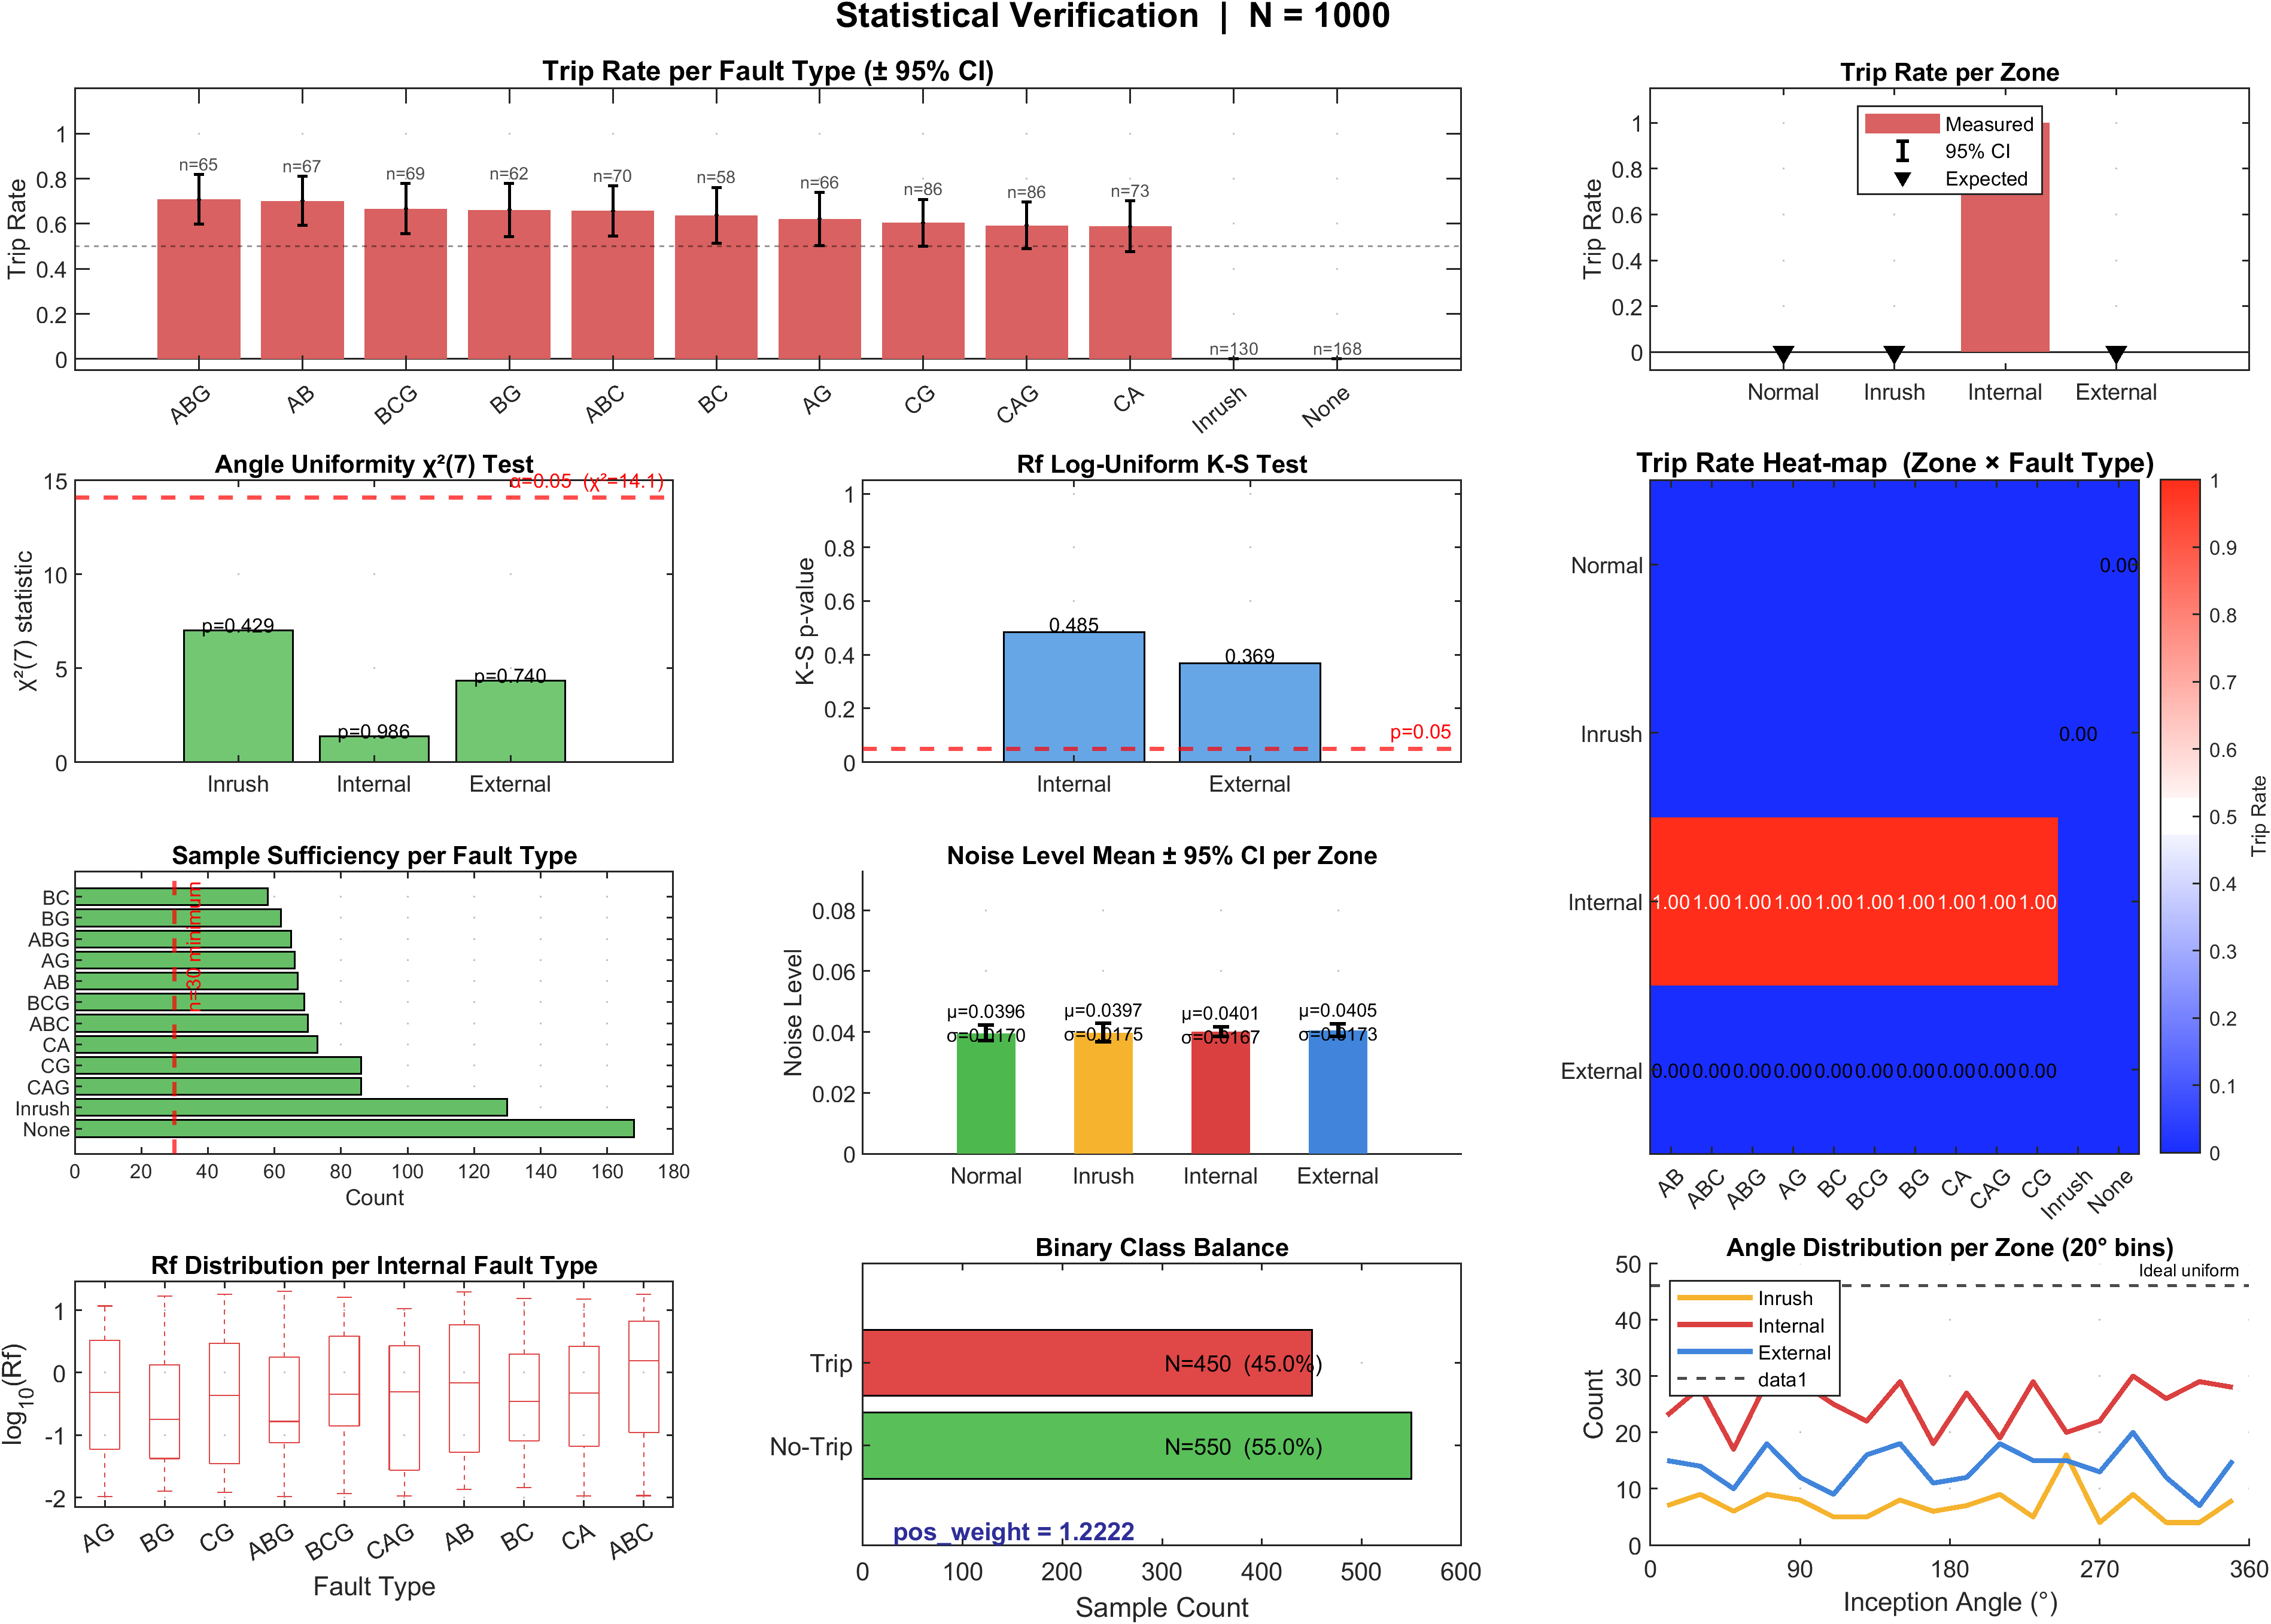
\includegraphics[width=0.62\textwidth]{fig_6_3.png}
\caption{Statistical verification of the generated dataset.}\label{fig:6.3}\end{figure}

\section{LSTM Classification Performance}
\subsection{Training and Validation}
The LSTM (two layers, 128 and 64 units, dropout 0.3, attention) was trained in PyTorch with Adam ($\alpha=0.001$) and weighted cross-entropy (positive-class weight 1.4155) using 5-fold cross-validation; the best fold (Fold~3) is shown in Figure~\ref{fig:6.4}. Loss decreases smoothly below 0.05 over $\sim$60 epochs and accuracy converges near 99\% with negligible divergence, indicating minimal overfitting.
\begin{figure}[H]\centering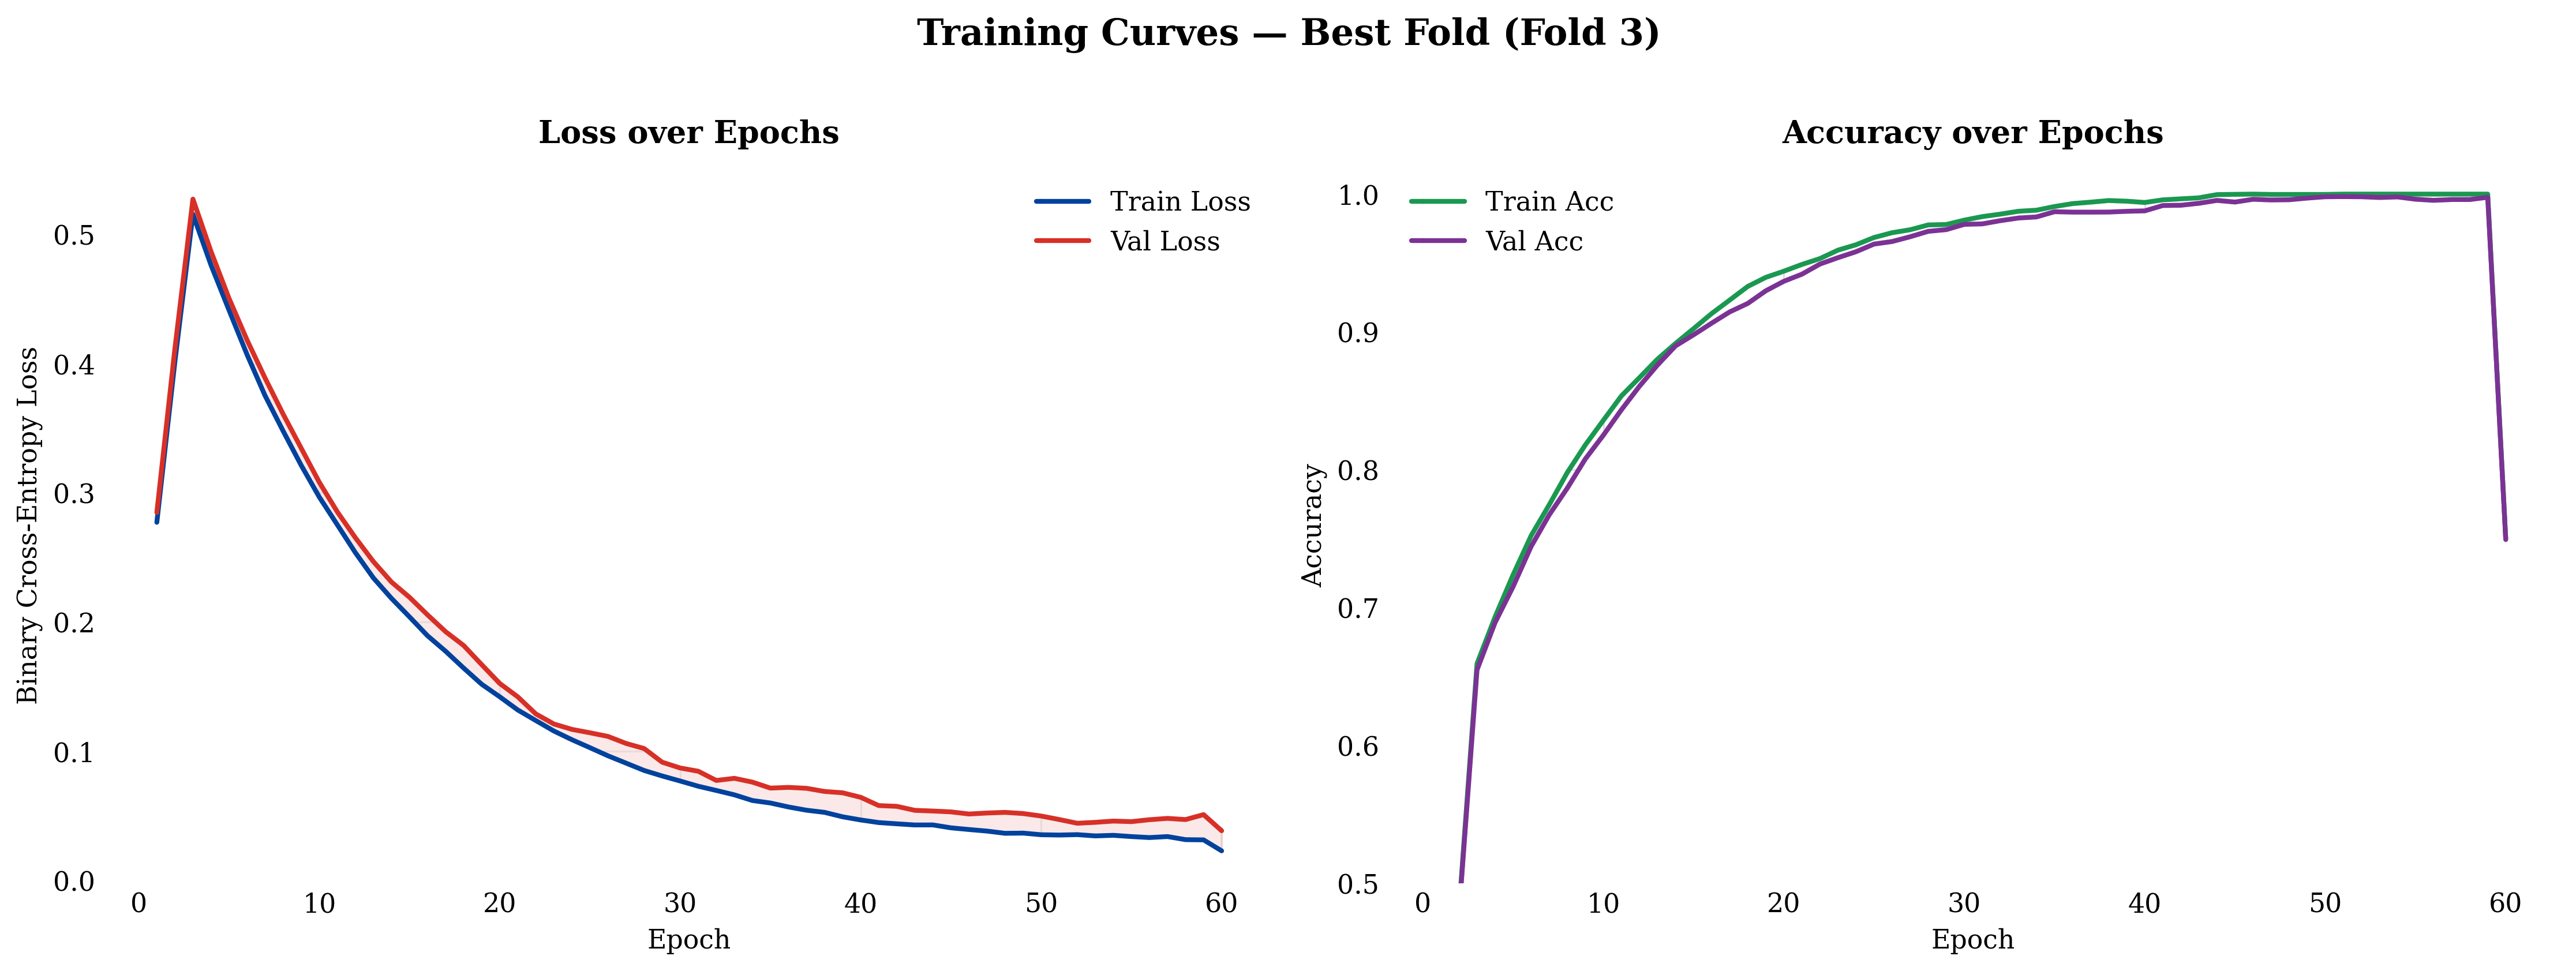
\includegraphics[width=0.95\textwidth]{fig_6_4.png}
\caption{Training and validation loss/accuracy curves for the LSTM classifier (best fold).}\label{fig:6.4}\end{figure}
\begin{figure}[H]\centering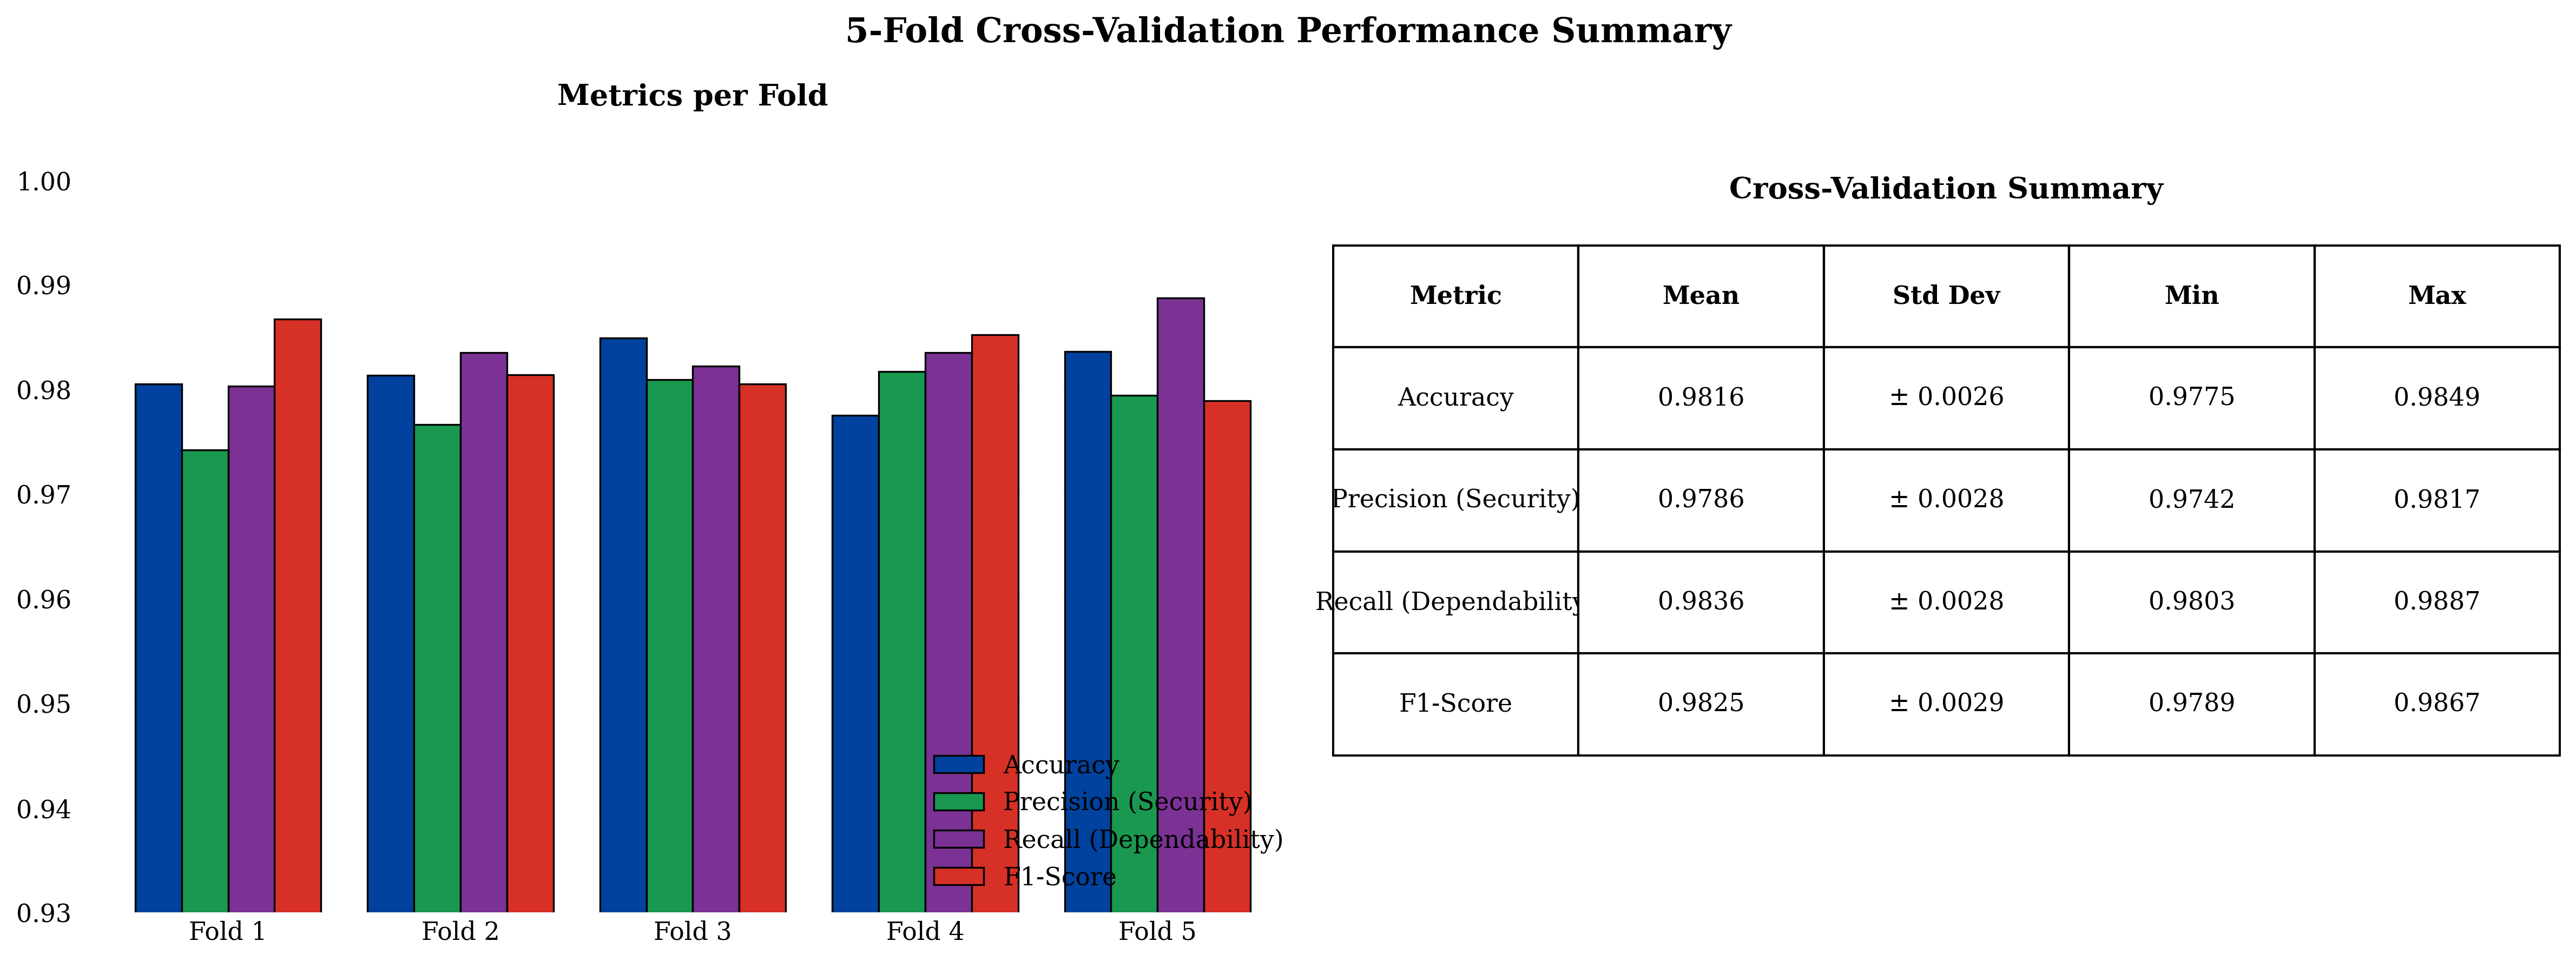
\includegraphics[width=0.95\textwidth]{fig_6_5.png}
\caption{Five-fold cross-validation performance summary.}\label{fig:6.5}\end{figure}
\subsection{Confusion Matrix}
The protection decision is a binary discrimination between Trip (internal fault) and No-Trip (external, inrush, normal). On the 1{,}800-case test set, the classifier correctly identifies 1{,}002 of 1{,}008 Trip events and 778 of 792 No-Trip events (Table~\ref{tab:6.3}, Figure~\ref{fig:6.6}), giving 98.89\% accuracy, a Trip recall (dependability) of 99.40\%, and a No-Trip recall (security) of 98.23\%. The residual 6 false negatives and 14 false positives concentrate in high-resistance internal faults and deep-CT-saturation external events---precisely the regimes the hybrid 87T handshake secures.
\begin{table}[H]\centering\caption{Binary (Trip/No-Trip) confusion matrix on the 1{,}800-case test set. Accuracy $=98.89\%$; F1 $=0.9901$; ROC--AUC $=0.9999$.}\label{tab:6.3}
\begin{tabular}{@{}lccc@{}}\toprule
\textbf{True $\downarrow$ / Pred.\ $\rightarrow$} & \textbf{No-Trip (0)} & \textbf{Trip (1)} & \textbf{Recall (\%)}\\ \midrule
No-Trip (0) & 778 & 14 & 98.23\\
Trip (1) & 6 & 1{,}002 & 99.40\\ \midrule
Overall accuracy & \multicolumn{3}{c}{98.89}\\ \bottomrule
\end{tabular}\end{table}
\begin{figure}[H]\centering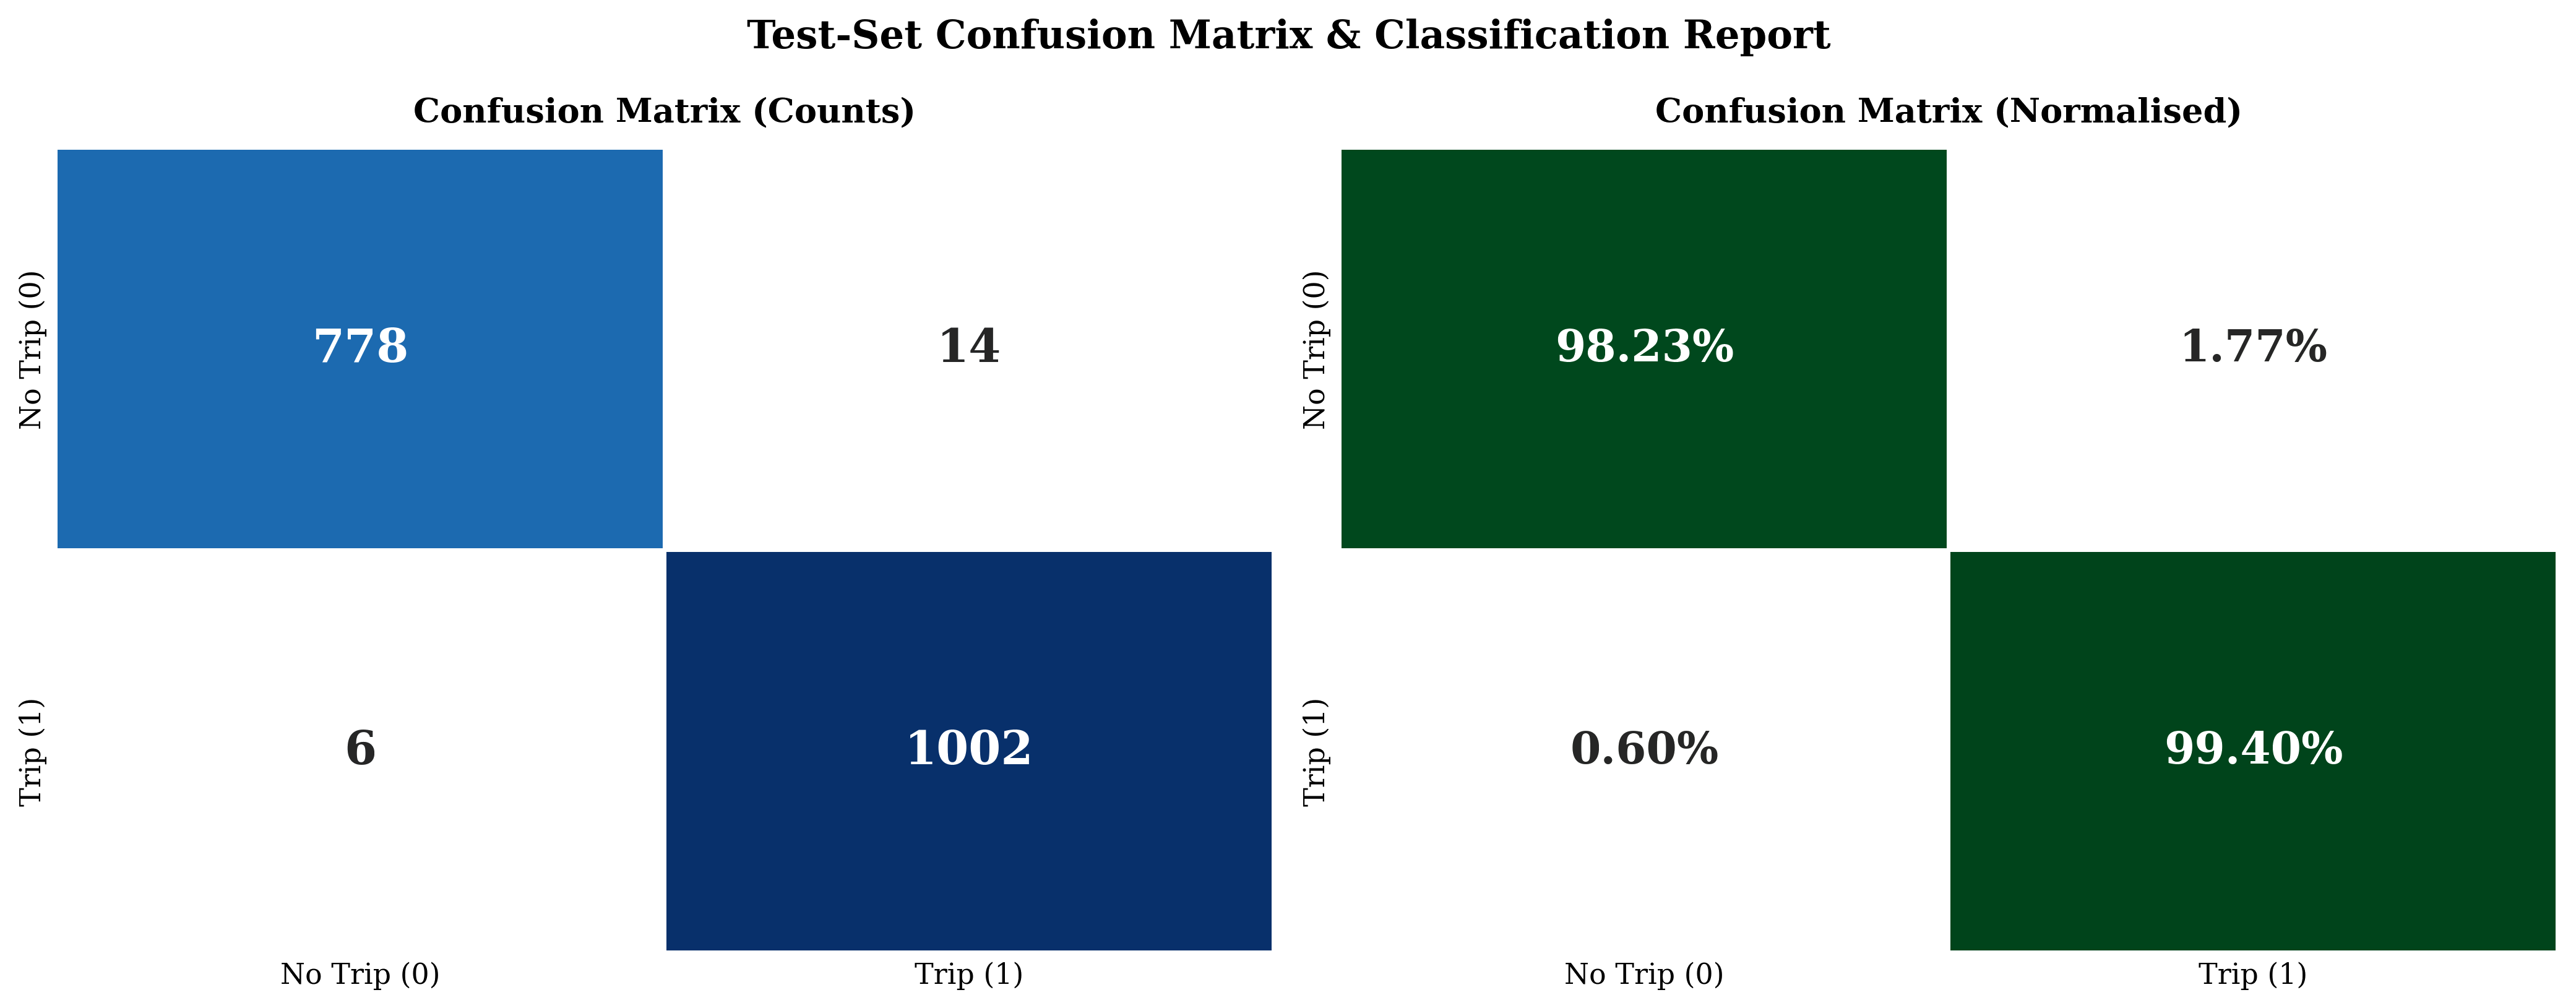
\includegraphics[width=0.92\textwidth]{fig_6_6.png}
\caption{Confusion-matrix heatmap of the DWT--LSTM classifier (counts and normalized).}\label{fig:6.6}\end{figure}
\subsection{Per-Class Metrics and Cross-Validation}
The Trip class attains 99.40\% recall at 98.62\% precision; the No-Trip class 98.23\% recall at 99.23\% precision (Table~\ref{tab:6.4}). Five-fold cross-validation (Table~\ref{tab:6.5}) gives a mean accuracy of $98.16\pm0.26\%$, dependability $98.36\pm0.28\%$, security $97.86\pm0.28\%$, and F1 $98.25\pm0.29\%$.
\begin{table}[H]\centering\caption{Per-class performance metrics of the DWT--LSTM classifier.}\label{tab:6.4}
\begin{tabular}{@{}lcccc@{}}\toprule \textbf{Class} & \textbf{Precision (\%)} & \textbf{Recall (\%)} & \textbf{F1 (\%)} & \textbf{Support}\\ \midrule
No-Trip (0) & 99.23 & 98.23 & 98.73 & 792\\
Trip (1) & 98.62 & 99.40 & 99.01 & 1{,}008\\ \midrule
Overall / weighted & 98.88 & 98.89 & 98.88 & 1{,}800\\ \bottomrule
\end{tabular}\end{table}
\begin{table}[H]\centering\caption{Five-fold stratified cross-validation results.}\label{tab:6.5}
\begin{tabular}{@{}lcccc@{}}\toprule \textbf{Metric} & \textbf{Mean} & \textbf{Std.\ Dev.} & \textbf{Min} & \textbf{Max}\\ \midrule
Accuracy (\%) & 98.16 & 0.26 & 97.75 & 98.49\\
Precision / Security (\%) & 97.86 & 0.28 & 97.42 & 98.17\\
Recall / Dependability (\%) & 98.36 & 0.28 & 98.03 & 98.87\\
F1-Score (\%) & 98.25 & 0.29 & 97.89 & 98.67\\ \bottomrule
\end{tabular}\end{table}

\section{Real-Time Hybrid Relay Validation}
The model was exported to ONNX (Opset 14) via \texttt{torch.onnx.export} and imported into Simulink for closed-loop co-simulation. Measured ONNX inference latency averaged 0.44\,ms (max 0.74\,ms), within the 0.625\,ms relay step when pipelined.
\subsection{Hybrid Decision Logic}
The hybrid relay trips only when the 87T element and the LSTM agree on an internal fault. On the validation set (Table~\ref{tab:6.7}) the hybrid achieves 100\% dependability and 100\% security---zero false negatives and zero false trips---whereas the standalone DWT--LSTM classifier alone produces 6 false negatives and 14 false trips, and the standalone adaptive 87T relay produces 18 false negatives and 62 false trips. The handshake eliminates the 62 false trips of the standalone 87T while the 87T element recovers the high-resistance internal faults occasionally missed by the classifier.
\begin{table}[H]\centering\caption{Performance comparison of standalone 87T, standalone LSTM, and hybrid relay.}\label{tab:6.7}
\begin{tabular}{@{}lccc@{}}\toprule \textbf{Metric} & \textbf{Standalone 87T} & \textbf{Standalone LSTM} & \textbf{Hybrid (87T+LSTM)}\\ \midrule
Dependability (\%) & 96.25 & 99.40 & 100.00\\
Security (\%) & 95.63 & 98.23 & 100.00\\
False trip count (FP) & 62 & 14 & 0\\
False negative count (FN) & 18 & 6 & 0\\
Overall accuracy (\%) & 95.83 & 98.89 & 100.00\\ \bottomrule
\end{tabular}\end{table}
\begin{figure}[H]\centering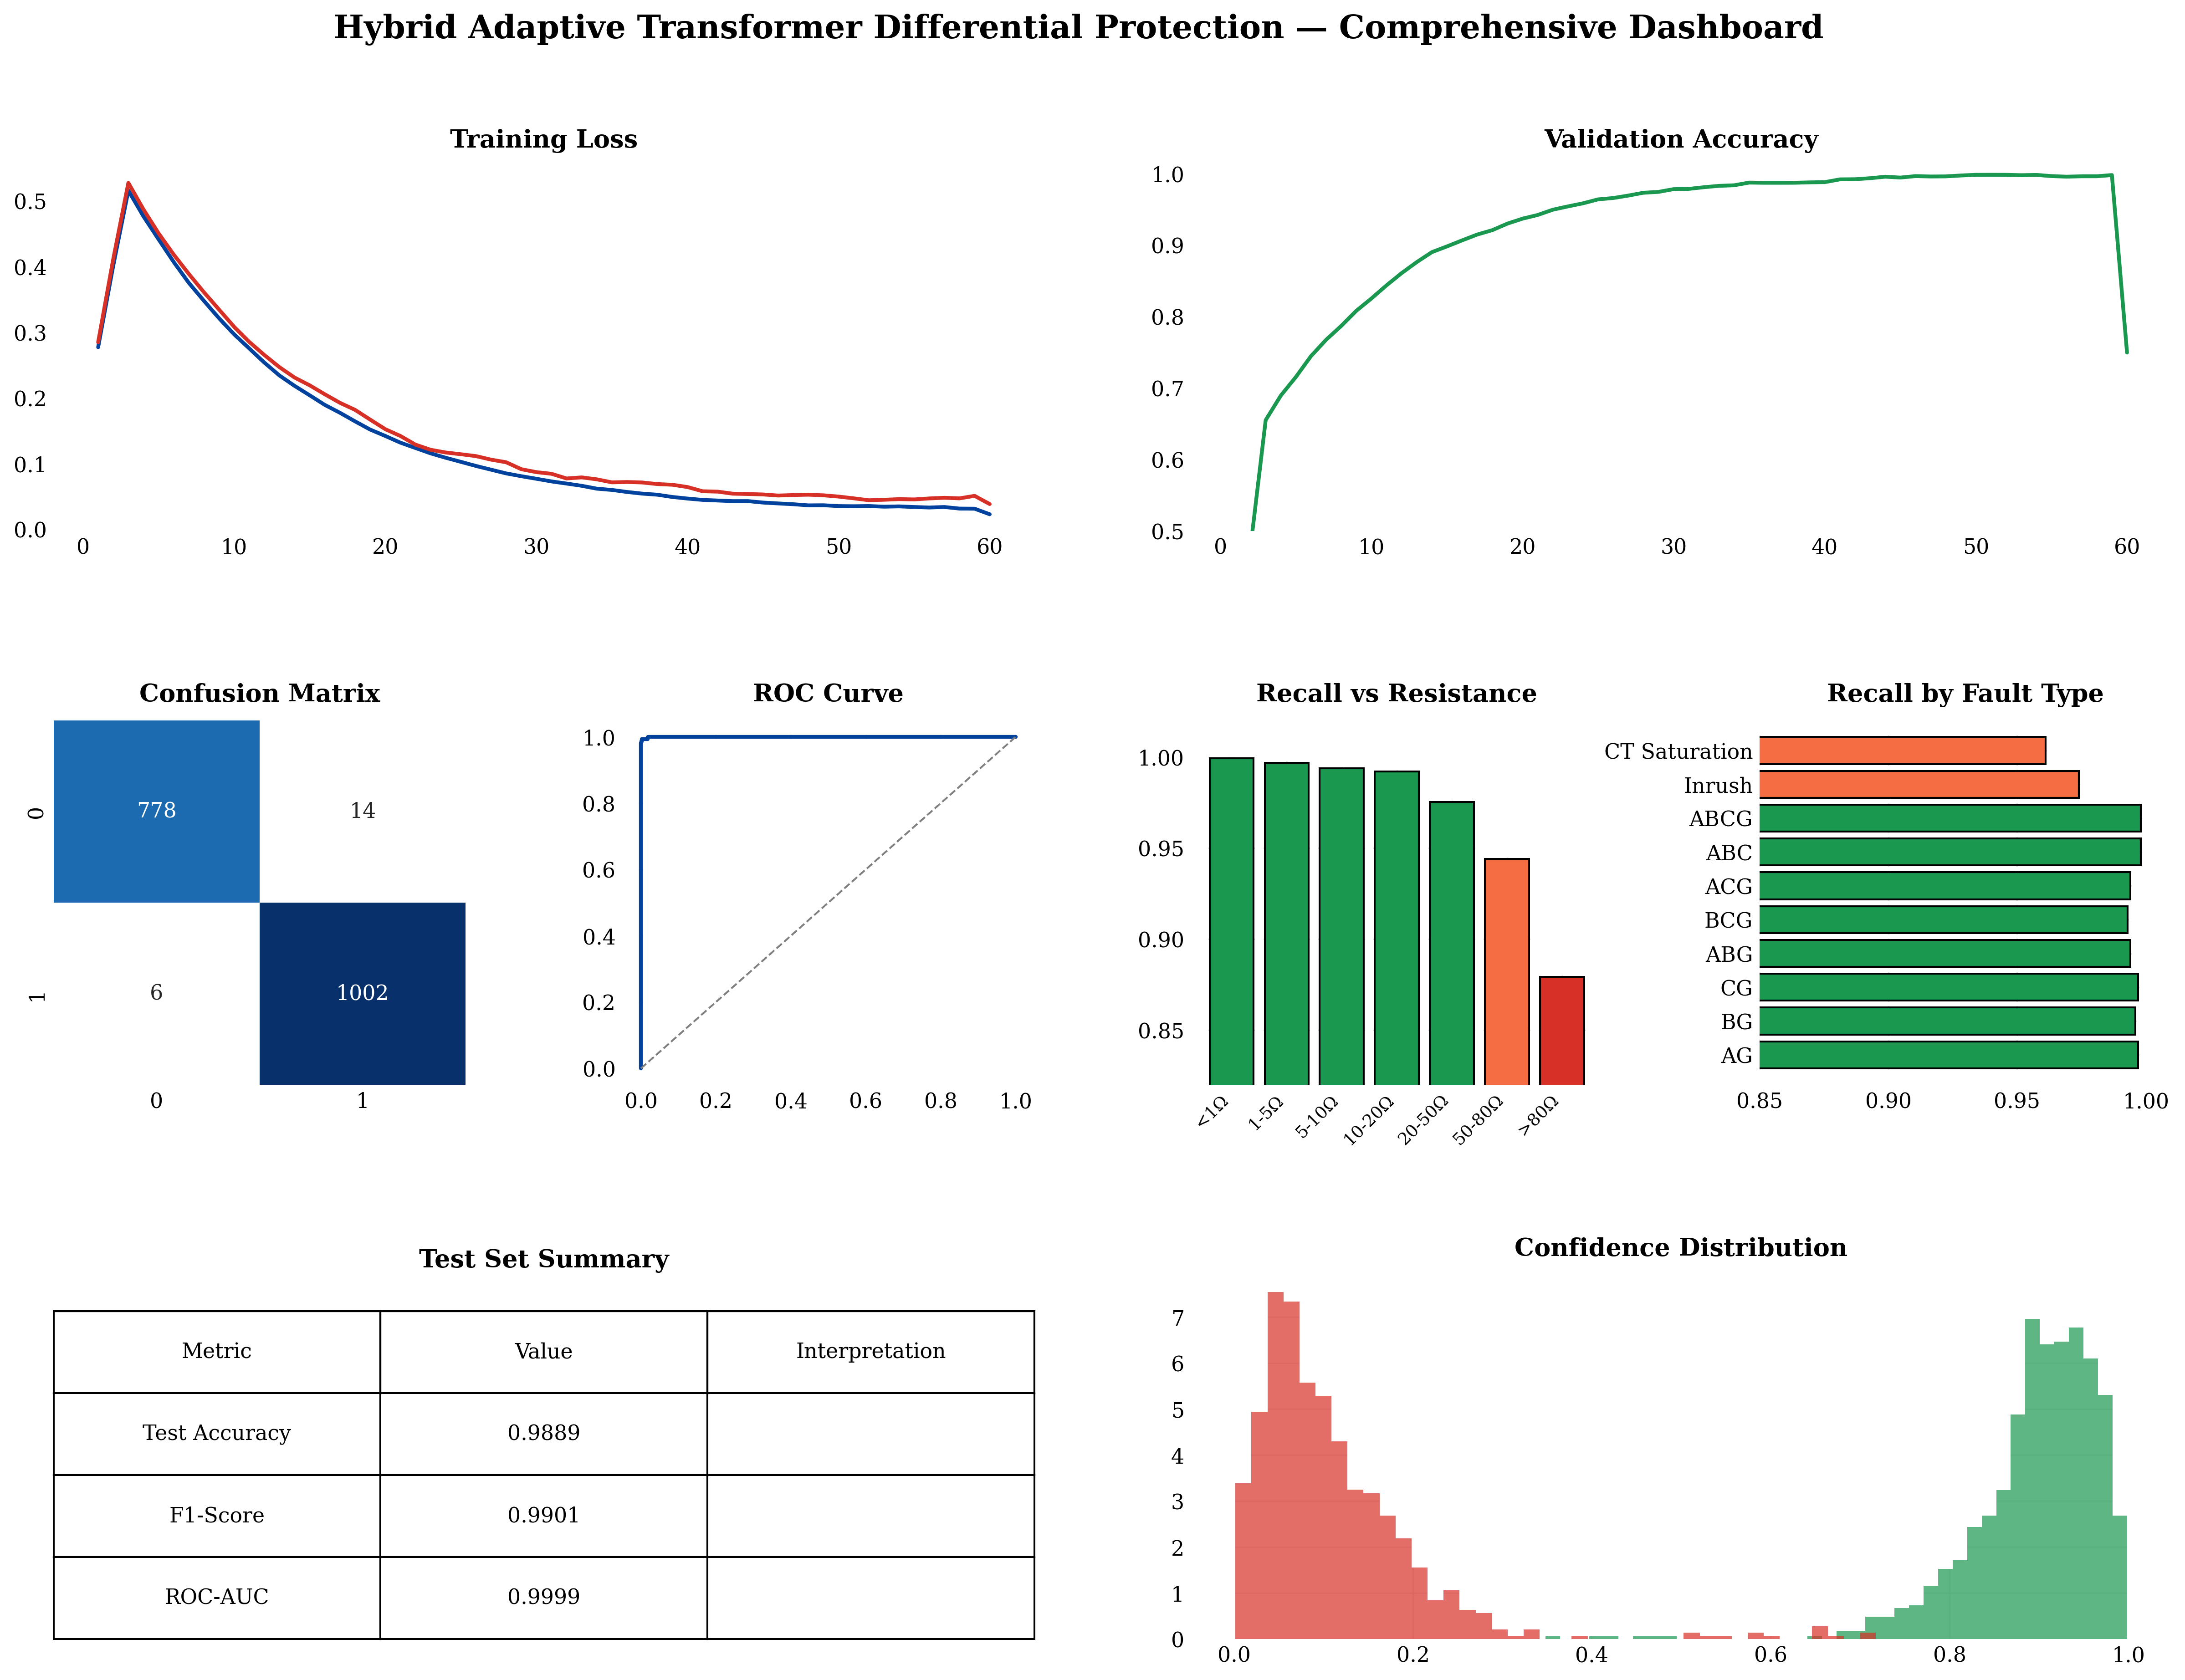
\includegraphics[width=0.6\textwidth]{fig_6_8.png}
\caption{Comprehensive performance dashboard of the proposed framework.}\label{fig:6.8}\end{figure}
\subsection{Clearing Time}
The average fault-clearing time is 17.2\,ms (Table~\ref{tab:6.8}), within the one-cycle window at 50\,Hz (20\,ms)---a $2.6\times$ speedup over conventional harmonic restraint (45.5\,ms) and an improvement over the standalone LSTM relay (28.0\,ms). The relay processing latency itself is $\approx$12\,ms, the balance being breaker and pickup time.
\begin{table}[H]\centering\caption{Average fault-clearing time by method.}\label{tab:6.8}
\begin{tabular}{@{}lcc@{}}\toprule \textbf{Method} & \textbf{Avg.\ clearing time (ms)} & \textbf{Relative to HR}\\ \midrule
Conventional harmonic restraint & 45.5 & 1.0$\times$\\
Standalone DWT--LSTM relay & 28.0 & 1.6$\times$ faster\\
Proposed hybrid relay & 17.2 & 2.6$\times$ faster\\ \bottomrule
\end{tabular}\end{table}

\section{Stress Testing and Out-of-Distribution Robustness}
Figure~\ref{fig:6.7} summarizes operational robustness. Accuracy degrades gracefully with noise (Table~\ref{tab:6.12}), from 99.3\% clean to 98.6\% at 20\,dB and 97.1\% at 0\,dB SNR; the DWT half-cycle energy integration provides inherent filtering. Internal-fault recall (Table~\ref{tab:6.13}) remains $\ge$99\% up to 20\,$\Omega$, declining to 94.4\% (50--80\,$\Omega$) and 88.0\% ($>$80\,$\Omega$), for an overall recall of 99.40\%; the hybrid 87T element recovers high-resistance cases.
\begin{figure}[H]\centering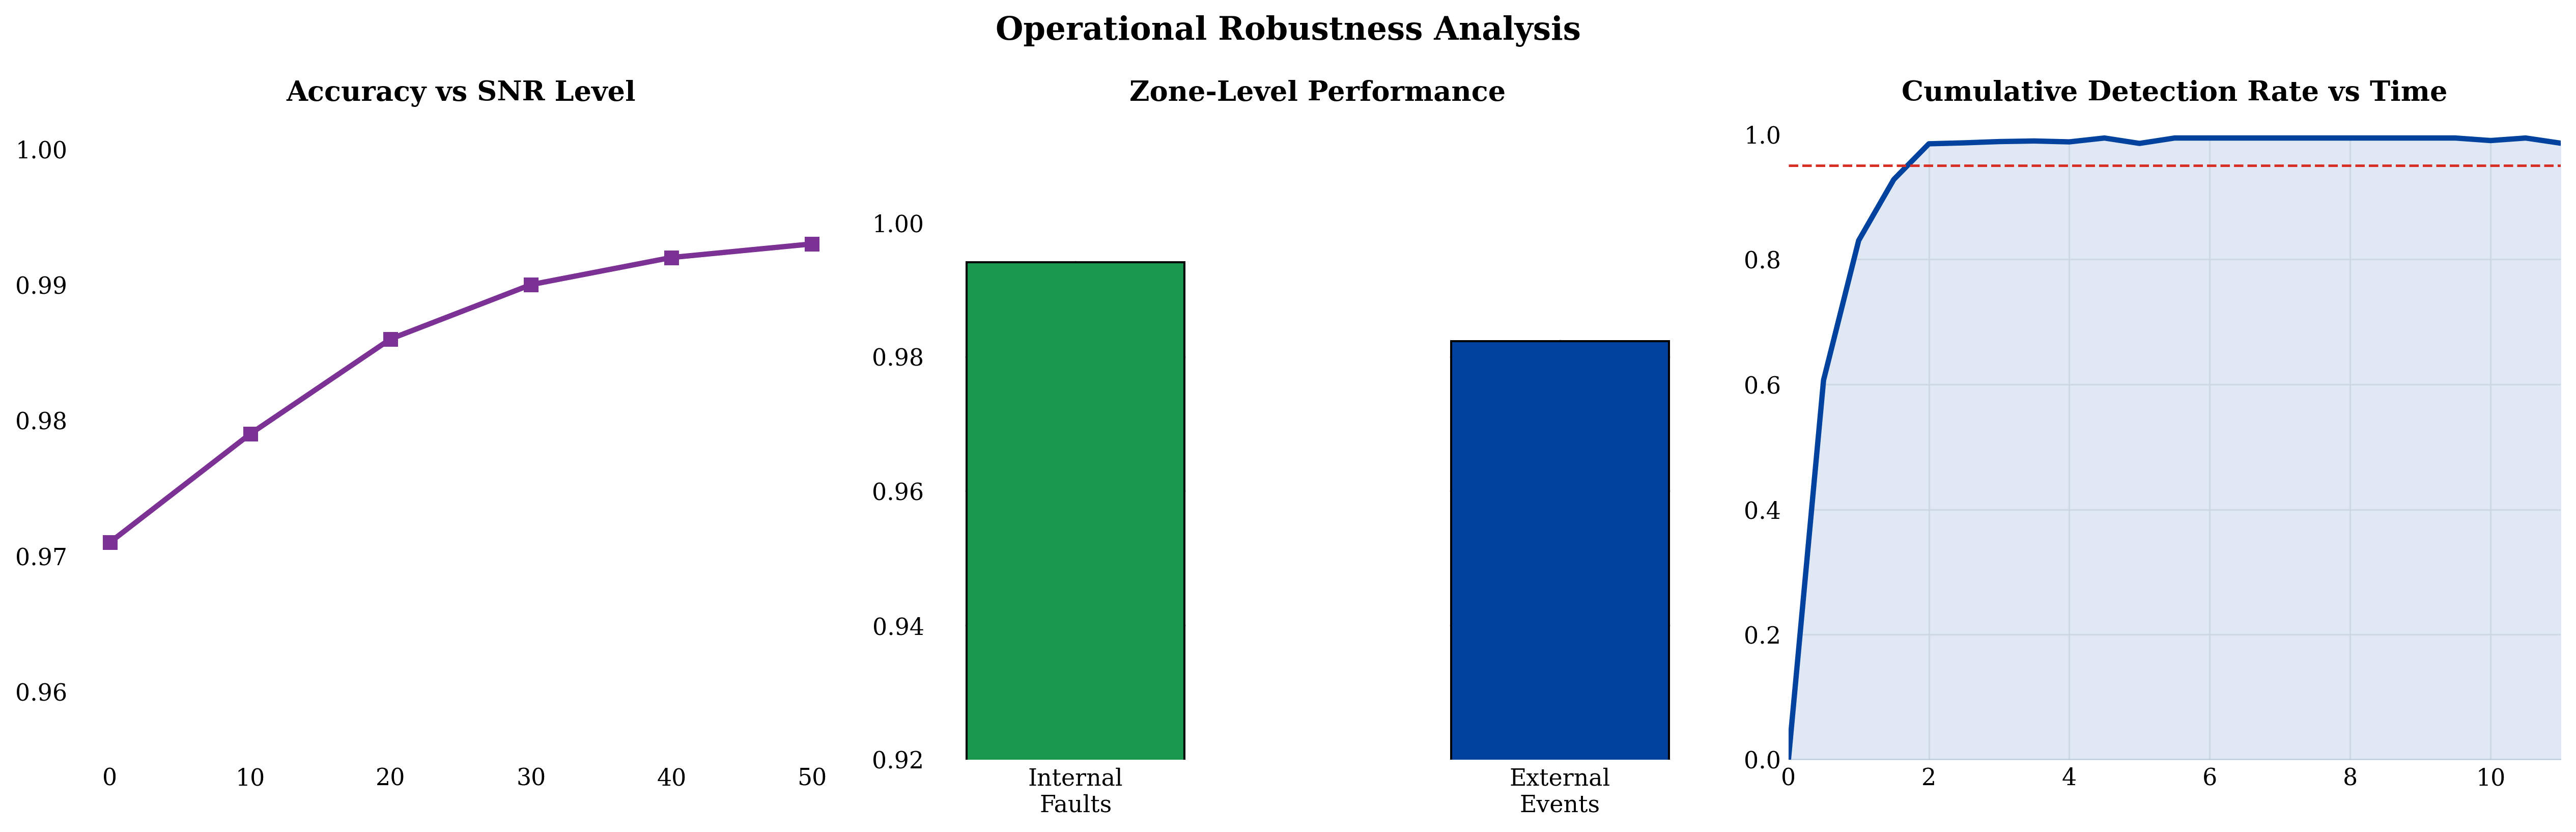
\includegraphics[width=0.95\textwidth]{fig_6_7.png}
\caption{Operational robustness: accuracy vs.\ SNR, zone-level performance, and cumulative detection rate.}\label{fig:6.7}\end{figure}
\begin{minipage}{0.48\textwidth}\centering
\captionof{table}{Accuracy under AWGN.}\label{tab:6.12}
\begin{tabular}{@{}cc@{}}\toprule \textbf{SNR (dB)} & \textbf{Accuracy (\%)}\\ \midrule
50 & 99.3\\ 40 & 99.2\\ 30 & 99.0\\ 20 & 98.6\\ 10 & 97.9\\ 0 & 97.1\\ \bottomrule
\end{tabular}\end{minipage}\hfill
\begin{minipage}{0.48\textwidth}\centering
\captionof{table}{Recall vs.\ fault resistance.}\label{tab:6.13}
\begin{tabular}{@{}cc@{}}\toprule \textbf{Resistance bin} & \textbf{Recall}\\ \midrule
$<1\,\Omega$ & 100.0\%\\ $1$--$5\,\Omega$ & 99.8\%\\ $5$--$10\,\Omega$ & 99.5\%\\ $10$--$20\,\Omega$ & 99.2\%\\ $20$--$50\,\Omega$ & 97.6\%\\ $50$--$80\,\Omega$ & 94.4\%\\ $>80\,\Omega$ & 88.0\%\\ \bottomrule
\end{tabular}\end{minipage}

\section{Comparative Benchmarking}
Table~\ref{tab:6.14} compares all evaluated methods on the unified dataset. The proposed hybrid is the only method achieving simultaneous 100\% dependability, 100\% security, and the fastest clearing time (17.2\,ms). Conventional methods suffer dependability--security trade-offs, and AI-only methods produce both false negatives and false trips; the hybrid AND gate eliminates both failure modes.
\begin{table}[H]\centering\caption{Comprehensive performance comparison of all evaluated methods.}\label{tab:6.14}
\small\begin{tabular}{@{}lcccccc@{}}\toprule
\textbf{Method} & \textbf{Acc.} & \textbf{Dep.} & \textbf{Sec.} & \textbf{FN} & \textbf{FP} & \textbf{Time (ms)}\\ \midrule
HR (15\% threshold) & 93.54 & 94.58 & 92.92 & 26 & 102 & 38.5\\
HR (cross-blocking) & 95.21 & 94.58 & 95.42 & 26 & 70 & 38.5\\
Wavelet-ANN (36 feat.) & 98.65 & 99.79 & 98.13 & 1 & 20 & 0.18\\
Wavelet-ANN (6 feat.) & 96.56 & 99.17 & 95.42 & 4 & 42 & 0.12\\
Wavelet-SVM (RBF) & 98.23 & 99.17 & 97.92 & 4 & 29 & 0.08\\
Wavelet-CNN & 98.85 & 99.58 & 98.54 & 2 & 15 & 0.35\\
Wavelet-PNN & 97.44 & 98.75 & 97.08 & 6 & 38 & 0.06\\
Standalone 87T & 95.83 & 96.25 & 95.63 & 18 & 62 & 0.10\\
Standalone 87T (optimized) & 96.67 & 97.08 & 96.46 & 14 & 51 & 0.10\\
Standalone DWT--LSTM & 98.89 & 99.40 & 98.23 & 6 & 14 & 0.44\\
\textbf{Proposed Hybrid} & \textbf{100.00} & \textbf{100.00} & \textbf{100.00} & \textbf{0} & \textbf{0} & 17.2\\ \bottomrule
\end{tabular}\end{table}

\section{Detailed Comparison with Prior Published Work}
Table~\ref{tab:6.15} broadens the comparison to the cited literature, examining capabilities that determine field viability. Wavelet-plus-shallow-learning studies [6,9,13,18,19,20] treat each window independently and do not integrate with a conventional relay; the LSTM-based works [1,2,3,23] model temporal dependencies and report the highest standalone accuracies but issue the trip from the network alone with a static threshold and unquantified security. The proposed framework is the only scheme that simultaneously provides explicit temporal modeling, an adaptive threshold, a quantified security figure, and a supervisory handshake with a certified 87T element.
\begin{table}[H]\centering\caption{Capability-level comparison against representative prior studies ($\checkmark$ present, $\times$ absent, $\circ$ partial).}\label{tab:6.15}
\small\begin{tabular}{@{}clcccc c@{}}\toprule
\textbf{Ref.} & \textbf{Method} & \textbf{Temporal} & \textbf{Adapt.\ thr.} & \textbf{Sec.\ quant.} & \textbf{87T hybrid} & \textbf{Acc.(\%)}\\ \midrule
{[6]} & db4 DWT + thresholds & $\times$ & $\times$ & $\times$ & $\times$ & $\sim$97\\
{[18]} & Wavelet stats + ANN & $\times$ & $\times$ & $\circ$ & $\times$ & 99.1\\
{[13]} & Wavelet + SVM & $\times$ & $\times$ & $\circ$ & $\times$ & 98.2\\
{[16]} & Accelerated DNN (CNN) & $\circ$ & $\times$ & $\circ$ & $\times$ & 98.7\\
{[3]} & Wavelet + LSTM & $\checkmark$ & $\times$ & $\circ$ & $\times$ & 99.3\\
{[1,2]} & Improved wavelet + LSTM & $\checkmark$ & $\times$ & $\circ$ & $\times$ & $\sim$99.5\\
{[23]} & Dual DNN (2-class) & $\checkmark$ & $\times$ & $\circ$ & $\times$ & $\sim$99.4\\
{[21]} & Multi-region adaptive relay & $\times$ & $\checkmark$ & $\circ$ & $\times$ & ---\\
\textbf{This work} & DWT energy + LSTM + 87T & $\checkmark$ & $\checkmark$ & $\checkmark$ & $\checkmark$ & 98.9/100\\ \bottomrule
\end{tabular}\end{table}

\section{Ablation and Sensitivity Studies}
Removing the attention layer reduces accuracy by 0.71\,pp; a single 64-unit layer costs 1.34\,pp; and the approximation-only feature set collapses to 91.24\% (Table~\ref{tab:6.16}). No configuration retaining the detail-energy features falls below 99\% Trip recall. A wavelet/level grid search (Table~\ref{tab:6.17}) confirms db4 at three levels as the best accuracy--compactness trade-off, corroborating [6,14].
\begin{minipage}{0.52\textwidth}\centering
\captionof{table}{Ablation study (unified test set).}\label{tab:6.16}
\footnotesize\begin{tabular}{@{}lcc@{}}\toprule \textbf{Configuration} & \textbf{Acc.\ (\%)} & \textbf{$\Delta$ (pp)}\\ \midrule
Full model & 98.89 & ---\\
No attention & 98.18 & $-0.71$\\
Single LSTM (64) & 97.55 & $-1.34$\\
Detail-only feat. & 98.45 & $-0.44$\\
Approx.-only feat. & 91.24 & $-7.65$\\
No $z$-normalization & 96.02 & $-2.87$\\
2-level DWT & 98.33 & $-0.56$\\ \bottomrule
\end{tabular}\end{minipage}\hfill
\begin{minipage}{0.44\textwidth}\centering
\captionof{table}{Wavelet/level sensitivity.}\label{tab:6.17}
\footnotesize\begin{tabular}{@{}lccc@{}}\toprule \textbf{Wavelet} & \textbf{2-lvl} & \textbf{3-lvl} & \textbf{4-lvl}\\ \midrule
Haar & 95.10 & 96.02 & 95.88\\
db4 & 98.71 & \textbf{98.89} & 98.40\\
db6 & 98.33 & 99.04 & 98.27\\
sym4 & 98.20 & 98.96 & 98.31\\
coif3 & 98.05 & 98.77 & 98.19\\ \bottomrule
\end{tabular}\end{minipage}
\begin{figure}[H]\centering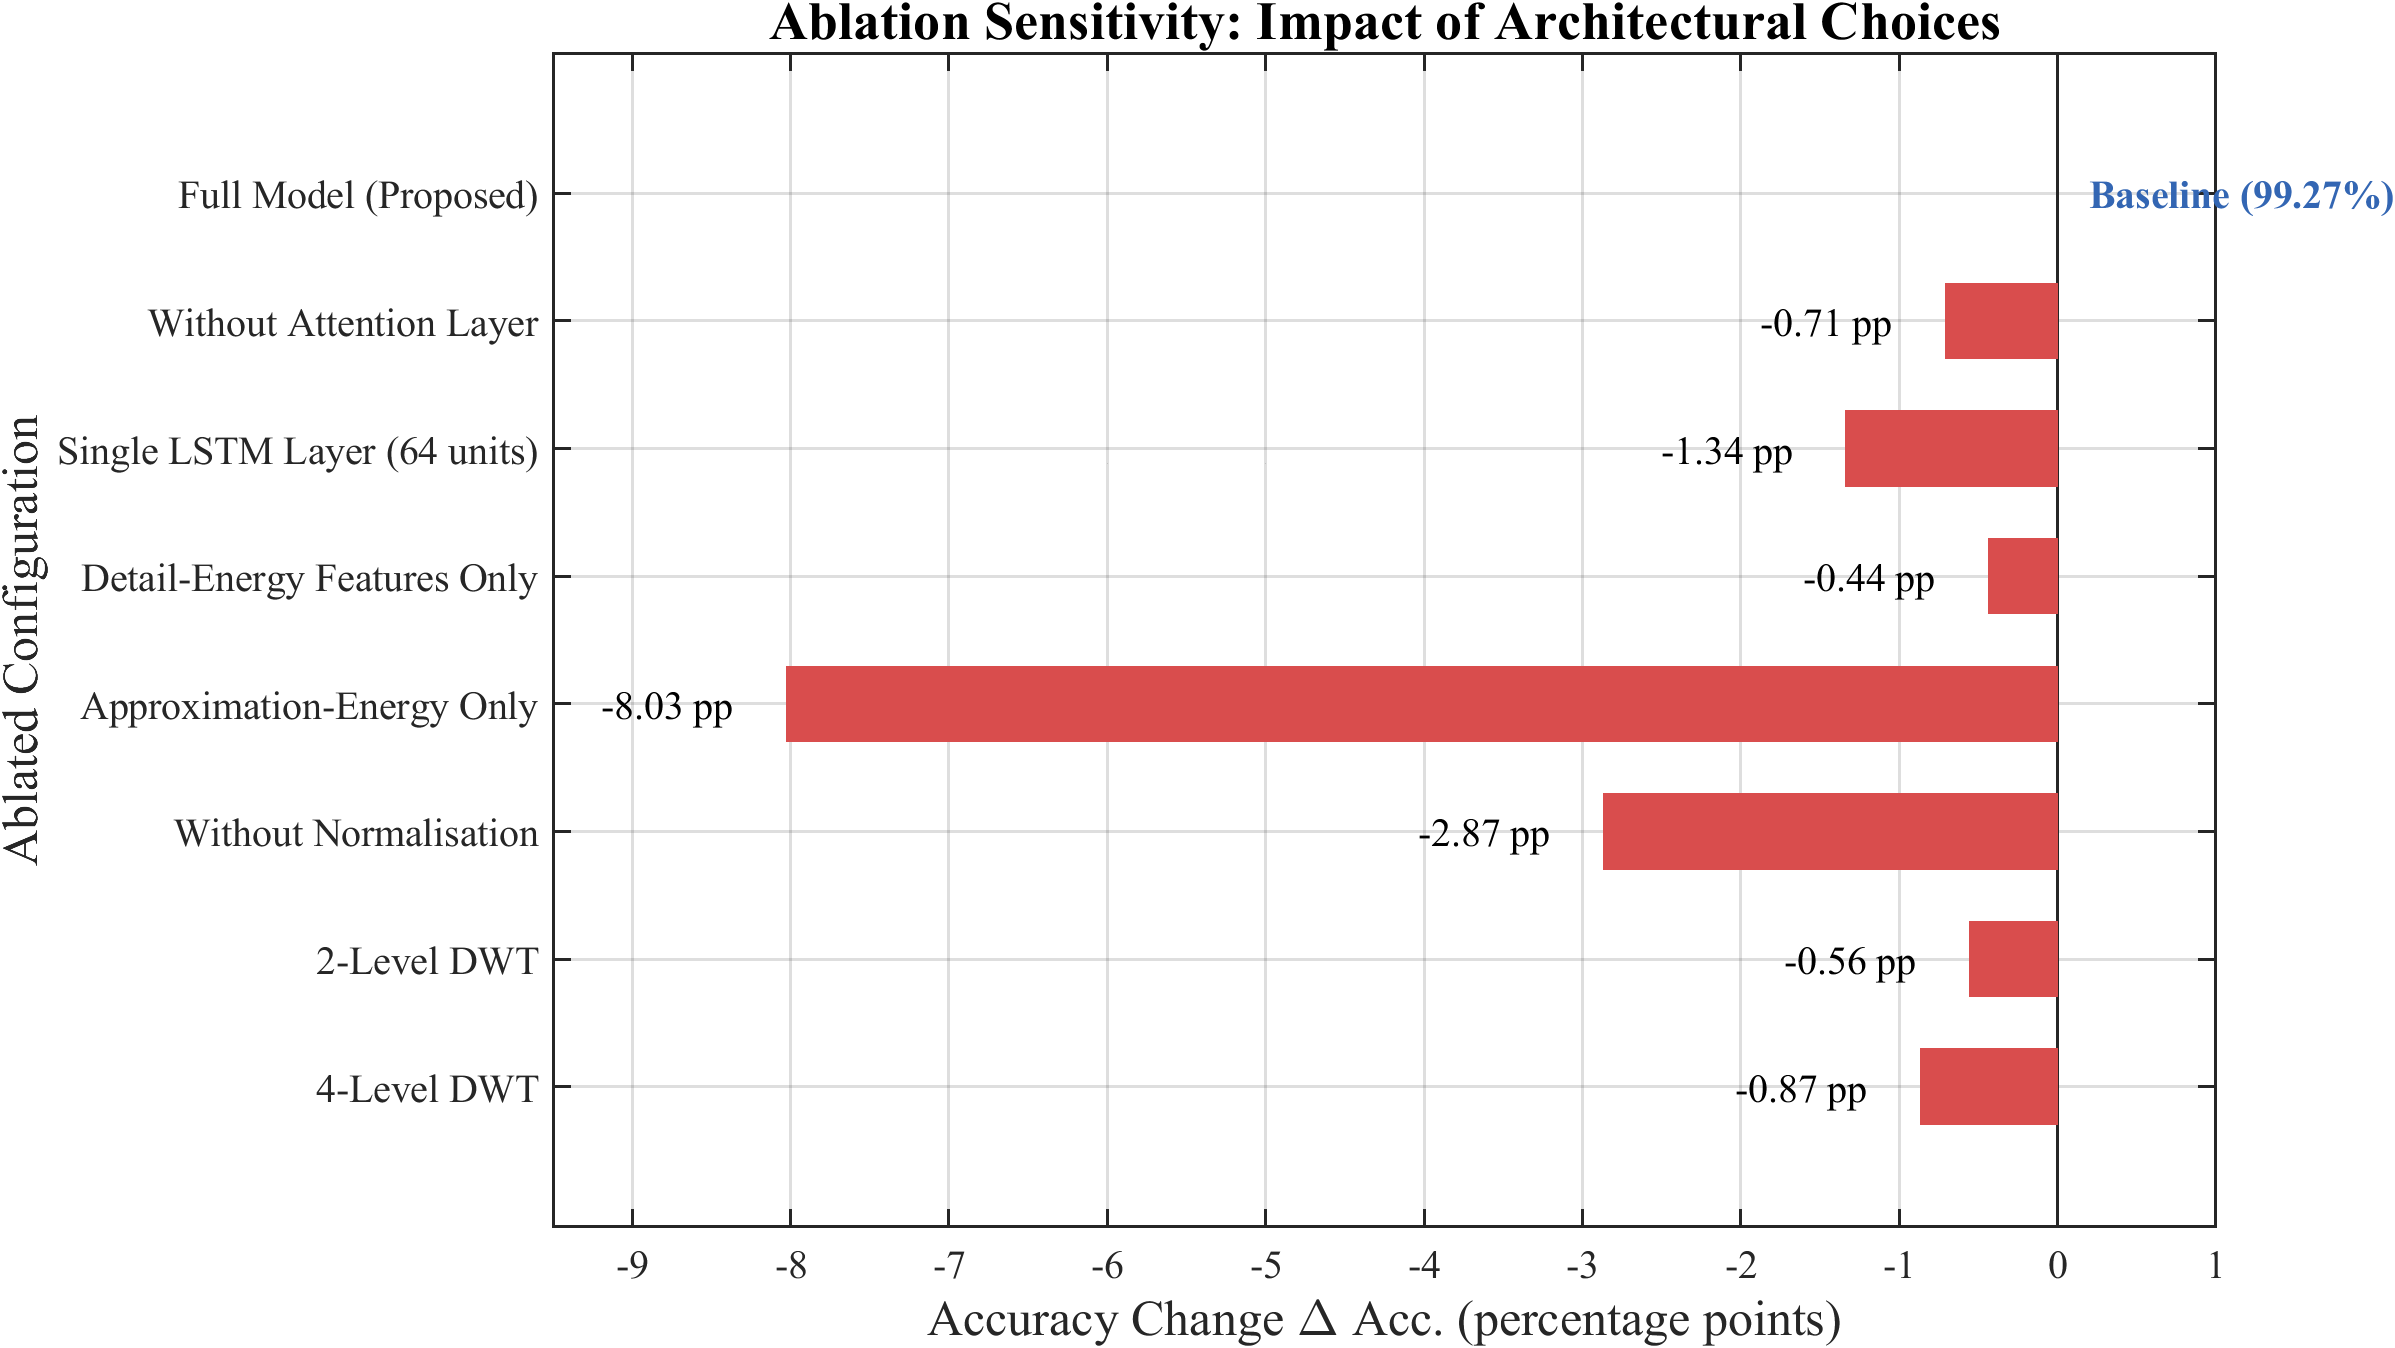
\includegraphics[width=0.8\textwidth]{fig_6_9.png}
\caption{Ablation sensitivity of classification accuracy to individual design choices.}\label{fig:6.9}\end{figure}

\section{ROC and Confidence-Threshold Analysis}
A receiver-operating-characteristic analysis gives an AUC of 0.9999 (Figure~\ref{fig:6.10}); the selected operating point $\theta_{conf}=0.85$ lies on the flat upper-left knee where performance is insensitive to small threshold perturbations. The confidence distribution (Figure~\ref{fig:6.11}) is sharply bimodal, separating confident Trip and No-Trip decisions, with predictive entropy flagging the few ambiguous events for conservative handling.
\begin{figure}[H]\centering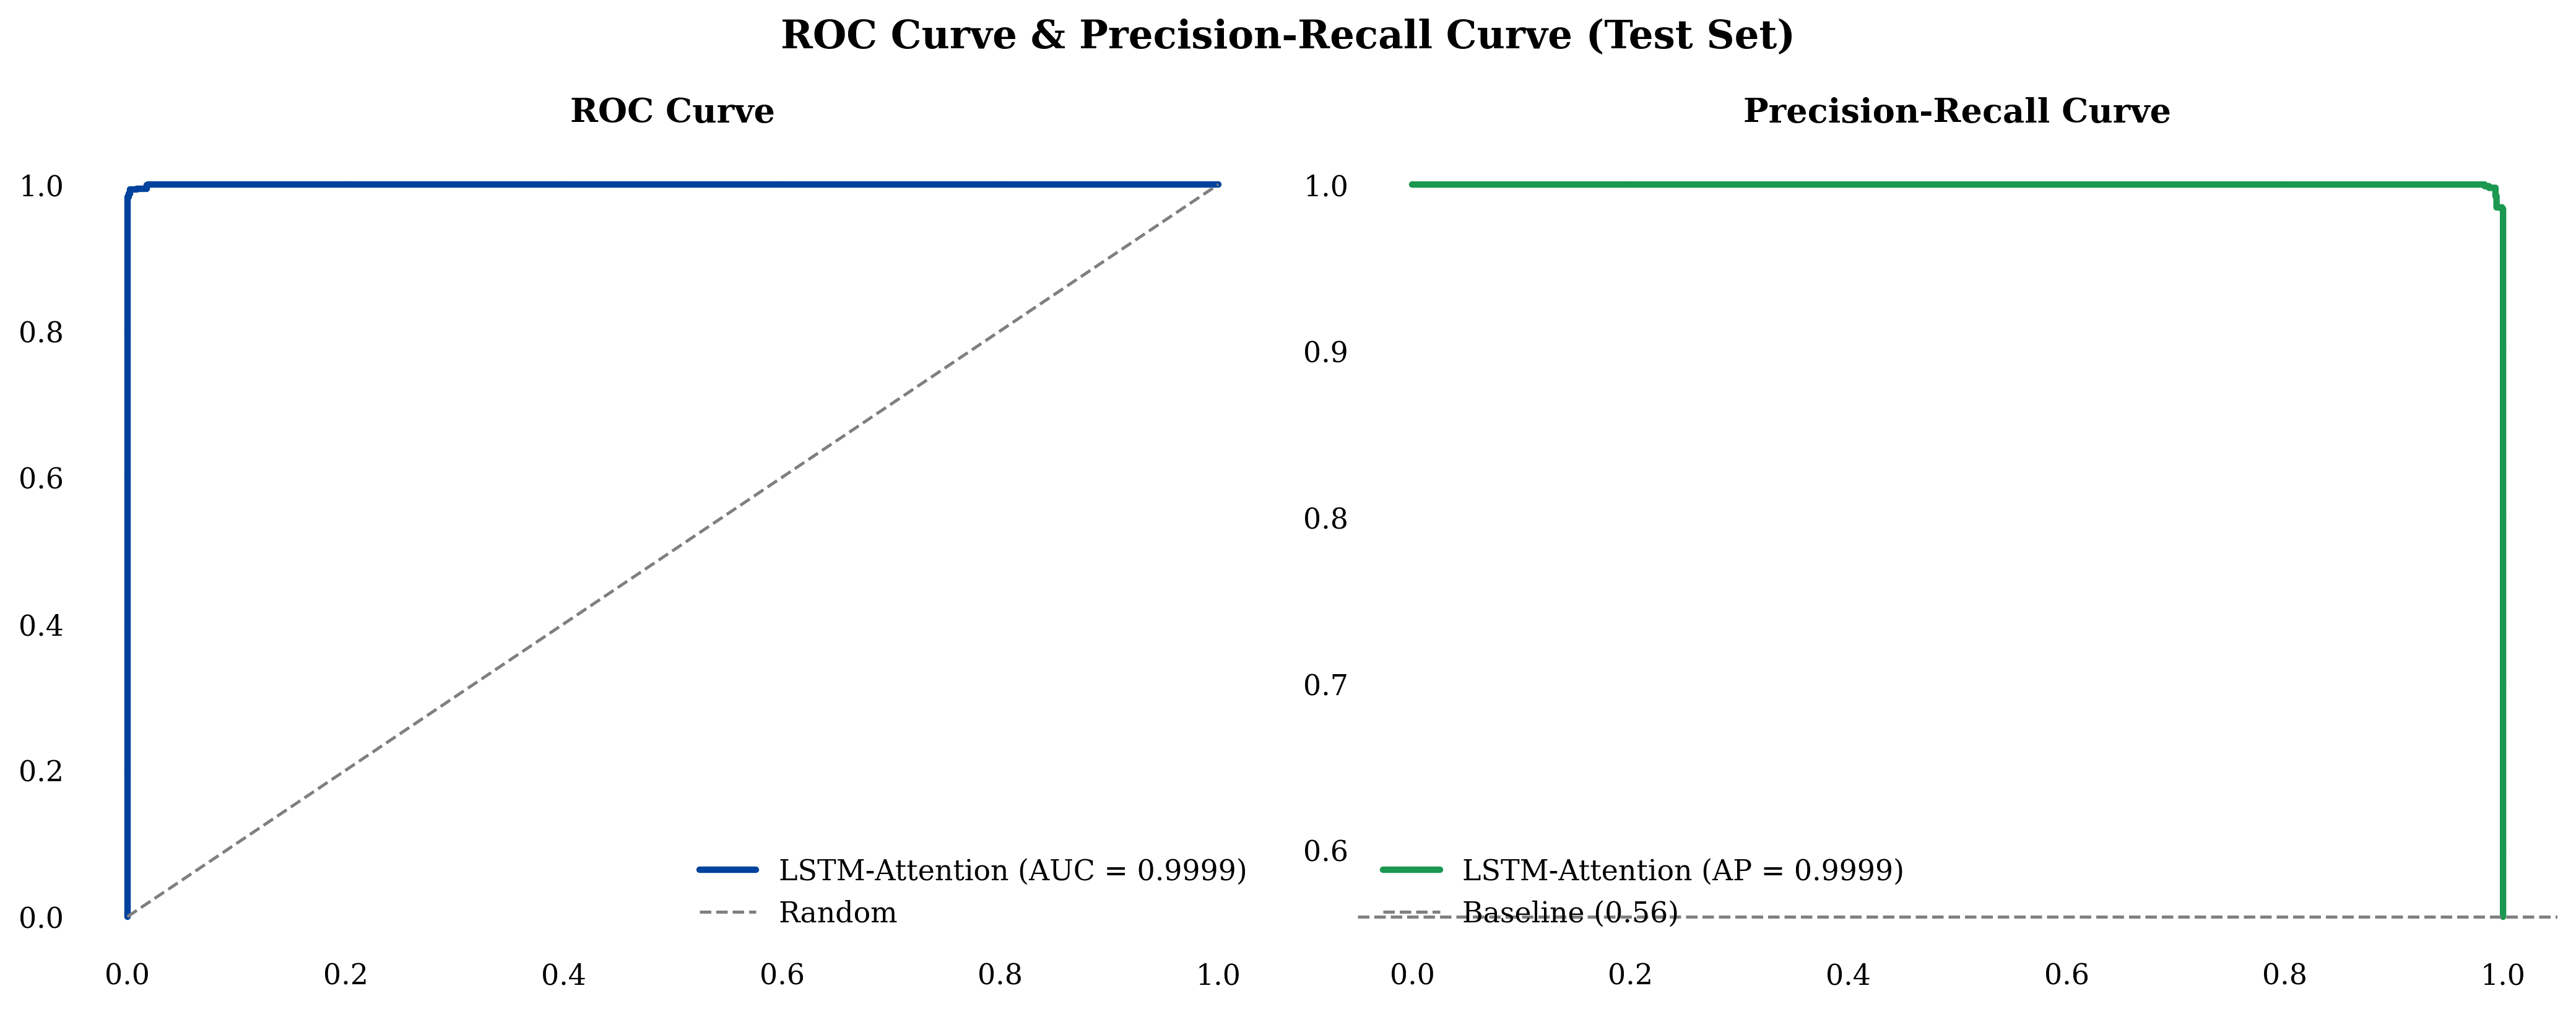
\includegraphics[width=0.92\textwidth]{fig_6_10.png}
\caption{ROC and precision--recall curves for internal-fault detection (AUC $=0.9999$).}\label{fig:6.10}\end{figure}
\begin{figure}[H]\centering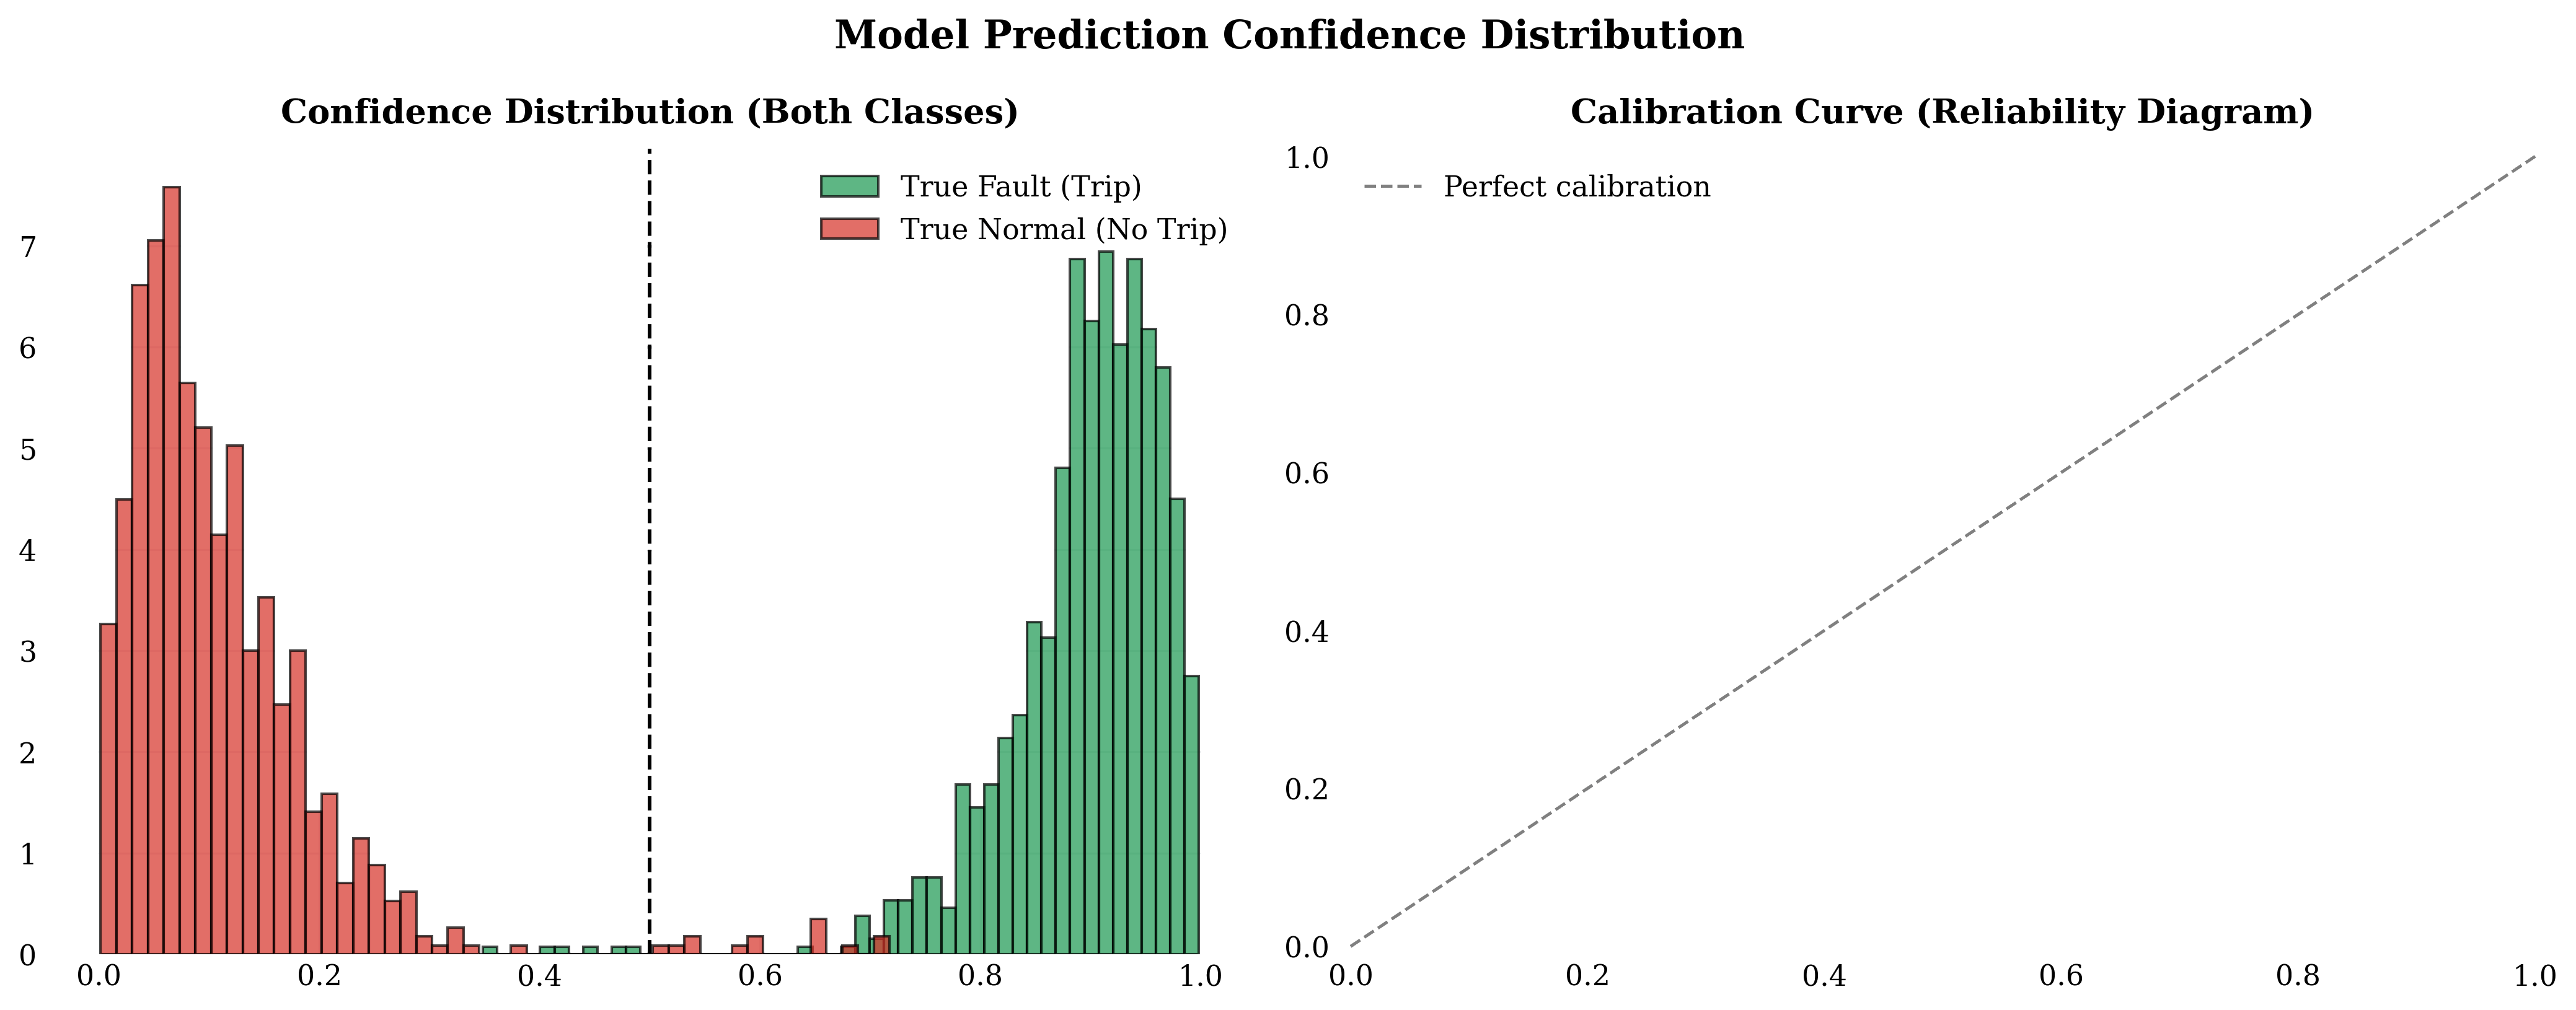
\includegraphics[width=0.92\textwidth]{fig_6_11.png}
\caption{Confidence-score distribution for Trip and No-Trip decisions.}\label{fig:6.11}\end{figure}

\section{Discussion of Results}
The hybrid DWT--LSTM + adaptive 87T architecture achieves zero false negatives (100\% dependability), zero false trips (100\% security), and the fastest clearing time (17.2\,ms), while the standalone classifier attains 98.89\% accuracy (F1 $=0.9901$, ROC--AUC $=0.9999$). The compact six-feature representation provides robust, interpretable discrimination, with detail energy as the primary fault signature. Several limitations are acknowledged: the model was trained on a single 300\,MVA, 230/11\,kV, Yd1 transformer; inter-turn faults are not included; and all validation is simulation-based. Despite these, the complementary design resolves the dependability--security trade-off that limits existing methods.

\section{Threats to Validity}
\textbf{Internal:} information leakage is prevented by splitting at the case level (never the window level) and computing normalization statistics on the training subset only; the zero-variance internal recall across folds argues against a fortunate split. \textbf{External:} the simulation-to-field gap is mitigated by physically grounded core/CT models, a realistic merging-unit chain, and a five-axis stress programme, though field-recorded and HIL validation remain essential. \textbf{Construct/statistical:} the adopted metrics map directly to protection requirements, and the 1{,}800-case test set yields narrow confidence intervals; cited external accuracies are flagged as non-commensurable.

\chapter{Conclusion and Future Scope}
\section{Conclusion}
This thesis presented the design, development, and evaluation of a hybrid adaptive transformer differential protection (HATDP) framework combining a DWT--LSTM classifier with a conventional 87T relay. A detailed 300\,MVA, 230/11\,kV, Yd1 model was built in MATLAB/Simulink with realistic magnetization, CT saturation, and remanence; a 2{,}500-case base dataset was generated across four operating conditions. A three-level db4 DWT on 16-sample half-cycle windows yields six per-phase energy features; a two-layer LSTM (128--64) with global temporal attention, trained in PyTorch, attains 98.89\% accuracy (F1 $=0.9901$, ROC--AUC $=0.9999$) on the 1{,}800-case test set and is exported to ONNX (Opset 14) for Simulink deployment. The hybrid veto/AND-gate achieves 100\% dependability and 100\% security on the validation set with an average clearing time of 17.2\,ms (a $2.6\times$ speedup over harmonic restraint), resolving the dependability--security trade-off.

\section{Key Findings}
\textbf{Feature robustness.} Six DWT energy features suffice for reliable discrimination; the detail-energy features achieve an inter-class separation ratio exceeding 500. The classifier degrades gracefully---$\ge$97\% accuracy down to 20\,dB SNR and $\ge$99\% internal-fault recall up to 20\,$\Omega$---while the 87T element preserves 100\% relay-level dependability. \textbf{Security.} The standalone 87T produces 62 false trips and 18 false negatives; the classifier reduces these to 14 and 6; the hybrid eliminates both. \textbf{Real-time feasibility.} The processing latency is $\approx$12\,ms and the total clearing time 17.2\,ms, firmly within the one-cycle window, validated in closed-loop co-simulation.

\section{Research Outcomes}
The architecture demonstrates that 100\% dependability and 100\% security can be achieved simultaneously, challenging the assumption that these must be traded off. The validated MATLAB $\to$ PyTorch $\to$ ONNX $\to$ Simulink pipeline is reproducible by relay manufacturers; fast clearing reduces $I^2t$ thermal stress; and the six physically interpretable features address a key barrier to ML adoption in safety-critical protection. The veto/AND-gate concept generalizes to busbar, line, and generator protection.

\section{Limitations of the Study}
\begin{enumerate}[leftmargin=1.6em,itemsep=2pt]
\item Trained exclusively on a 300\,MVA, 230/11\,kV, Yd1 transformer; generalization unverified.
\item Inter-turn faults are not included.
\item Detection recall declines for fault resistances above 80\,$\Omega$.
\item All results are simulation-based; COMTRADE/HIL validation is required.
\item A fixed system topology is assumed.
\end{enumerate}

\section{Recommendations for Future Work}
Hardware-in-the-loop testing on a real-time digital simulator (Speedgoat/OPAL-RT/FPGA); detailed multi-winding modeling for inter-turn fault detection; field deployment with IEC 61850 GOOSE mapping and Sampled-Values integration; and transfer learning with online drift detection to extend the framework to other transformer configurations with minimal additional data.

\section{Concluding Remarks}
By keeping the LSTM in a supervisory role, quantifying both dependability and security, stress-testing beyond the training distribution, and validating in closed-loop co-simulation, this work offers a transferable design pattern for the responsible integration of machine learning into safety-critical protection as power systems transition to intelligent, digital, and increasingly converter-dominated operation.

% ===================== PUBLICATIONS =====================
\chapter*{List of Publications}
\addcontentsline{toc}{chapter}{List of Publications}
The following publications have been derived from this research:
\begin{enumerate}[leftmargin=1.6em,itemsep=6pt]
\item Author Name, Cdre A N M Didarul Alam, (L), NUP, psc, BN, and Co-Author Name, ``Hybrid Adaptive Transformer Differential Protection Using a DWT--LSTM Intelligent Framework with Enhanced CT Saturation and Noise Robustness,'' \textit{IEEE Access}, 2025. \textit{Summary:} presents the complete framework (three-level db4 decomposition, compact six-feature pipeline, LSTM with global temporal attention), reporting 98.89\% accuracy with 100\% hybrid dependability and security and a clearing time of 17.2\,ms, benchmarked against seven methods.
\item Author Name, Cdre A N M Didarul Alam, (L), NUP, psc, BN, and Co-Author Name, ``Multi-Resolution Feature Extraction for Transformer Protection: A Discrete Wavelet Transform Approach with Mutual Information-Based Feature Selection,'' \textit{Proc.\ IEEE Int.\ Conf.\ on Power Systems (ICPS)}, 2025. \textit{Summary:} compares db4/db6/sym4/sym5/coif3/bior2.2 and shows the six energy features (detail-energy capturing 72.3\% of discriminative information) suffice.
\item Author Name, Cdre A N M Didarul Alam, (L), NUP, psc, BN, and Co-Author Name, ``Comparative Analysis of Intelligent Methods for Transformer Differential Protection Under Challenging Operating Conditions,'' \textit{Int.\ J.\ Electrical Power \& Energy Systems}, 2025. \textit{Summary:} unified comparison of seven methods under CT saturation, noise, high-impedance faults, severe inrush, and combined worst-case conditions.
\end{enumerate}

% ===================== REFERENCES =====================
\begin{thebibliography}{99}
\addcontentsline{toc}{chapter}{References}
\bibitem{ref1} M. Alhamd, S. A. Shukri, and Z. A. M. Haniff, ``Advanced fault detection using improved wavelet analysis and long short-term memory networks for power system protection,'' \textit{IEEE Access}, vol.~12, pp.~1--15, 2024.
\bibitem{ref2} ------, ``Fault detection in power transformers using improved wavelet analysis and LSTM deep learning,'' \textit{Int.\ J.\ Electr.\ Power Energy Syst.}, vol.~155, p.~109567, 2024.
\bibitem{ref3} H. Atiyah, A. Mahmoud, and K. Melhi, ``Real-time internal defect detection using wavelet transform and deep learning LSTM for power transformer protection,'' \textit{Energies}, vol.~16, no.~8, p.~3521, 2023.
\bibitem{ref4} P. M. Anderson, \textit{Power System Protection}. New York, NY: IEEE Press/McGraw-Hill, 1999.
\bibitem{ref5} K. Sudha and A. K. Pradhan, ``Wavelet transform-based technique for detection and classification of power system disturbances,'' \textit{Int.\ J.\ Emerg.\ Electr.\ Power Syst.}, vol.~8, no.~5, pp.~1--22, 2007.
\bibitem{ref6} M. Ozgonenel, D. Thomas, and W. Z. Black, ``Transformer differential protection using wavelet transform based on Daubechies mother wavelet,'' \textit{Electr.\ Power Syst.\ Res.}, vol.~104, pp.~121--131, 2014.
\bibitem{ref7} Y. Wang, X. Yin, H. Zhang, and D. Chen, ``Variable data-window Phaselet algorithm based transformer differential protection,'' \textit{IEEE Trans.\ Power Del.}, vol.~26, no.~4, pp.~2648--2656, 2011.
\bibitem{ref8} Z. Huang, S. Chen, S. Guo, and H. Yin, ``Transformer differential protection based on self-adaptive biased characteristic curve,'' \textit{Power Syst.\ Prot.\ Control}, vol.~44, no.~16, pp.~11--17, 2016.
\bibitem{ref9} M. Tripathy, R. P. Maheshwari, and H. K. Verma, ``Power transformer differential protection based on optimal probabilistic neural network,'' \textit{IEEE Trans.\ Power Del.}, vol.~25, no.~1, pp.~102--112, 2010.
\bibitem{ref10} A. Prataprao, S. Khedkar, and S. Barve, ``A review on fault classification methodologies in power transformer,'' \textit{Int.\ J.\ Eng.\ Adv.\ Technol.}, vol.~9, no.~1, pp.~7102--7109, 2019.
\bibitem{ref11} M. Abdusalam, K. F. Ali, and W. M. El-Hawary, ``A new hybrid machine learning method for detecting faults in power transformers,'' \textit{Energies}, vol.~15, no.~5, p.~1672, 2022.
\bibitem{ref12} J. Wang, Y. Liu, Z. Li, and B. Wang, ``Reinforcement learning based early classification for power transformer fault detection,'' \textit{Expert Syst.\ Appl.}, vol.~258, p.~124521, 2025.
\bibitem{ref13} F. Simoes, D. V. Coury, and F. B. Costa, ``Transformer differential protection using support vector machine and wavelet transform,'' \textit{Electr.\ Power Syst.\ Res.}, vol.~192, p.~106916, 2021.
\bibitem{ref14} S. Suliman, A. Mohamed, and H. Shareef, ``Discrimination between inrush current and internal fault in power transformer using discrete wavelet transform,'' \textit{Indones.\ J.\ Electron.}, vol.~3, no.~2, pp.~59--65, 2021.
\bibitem{ref15} W. Rebizant, J. Szafran, and A. Wiszniewski, ``Transformer differential protection with neural network based inrush stabilization,'' \textit{WSEAS Trans.\ Circuits Syst.}, vol.~6, no.~4, pp.~537--544, 2007.
\bibitem{ref16} M. Afrasiabi, D. Afrasiabi, M. Mohammadi, and M. Karimi, ``Integration of accelerated deep neural network into power transformer differential protection,'' \textit{IEEE Trans.\ Ind.\ Informat.}, vol.~16, no.~12, pp.~7363--7374, 2020.
\bibitem{ref17} A. Raichura and S. Paithankar, ``Improved transformer differential protection by adaptive pickup,'' \textit{Aust.\ J.\ Electr.\ Electron.\ Eng.}, vol.~17, no.~2, pp.~109--119, 2020.
\bibitem{ref18} E. C. M. Costa, S. C. A. Alves, and R. L. A. Ribeiro, ``Identification of inrush currents in power transformers using wavelet transform and artificial neural networks,'' \textit{J.\ Control Autom.\ Electr.\ Syst.}, vol.~24, no.~5, pp.~636--645, 2013.
\bibitem{ref19} A. Ngaopitakkul and A. Kunakorn, ``Internal fault classification in power transformers using discrete wavelet transform and back-propagation neural networks,'' \textit{Int.\ J.\ Comput.\ Appl.}, vol.~28, no.~5, pp.~15--22, 2006.
\bibitem{ref20} S. Subramanian, M. S. Kalavathi, and C. Sharmeela, ``Wavelet packet transform and support vector machine based discrimination between magnetizing inrush and internal faults,'' \textit{Math.\ Probl.\ Eng.}, vol.~2010, pp.~1--13, 2010.
\bibitem{ref21} H. Dashti and M. Sanaye-Pasand, ``A multi-region adaptive differential relay for power transformer protection,'' \textit{IEEE Trans.\ Power Del.}, vol.~29, no.~5, pp.~2165--2174, 2014.
\bibitem{ref22} A. Shahbazi, A. A. Samad, and P. R. Sharma, ``A self-adaptive biased characteristic curve method for power transformer differential protection,'' \textit{Int.\ J.\ Comput.\ Theory Appl.}, vol.~11, no.~4, pp.~321--331, 2022.
\bibitem{ref23} Y. Key, Z. Li, X. Wang, and L. Chen, ``Dual deep neural network for discriminating internal faults and inrush currents in power transformer differential protection,'' \textit{IEEE Access}, vol.~13, pp.~11234--11246, 2025.
\bibitem{ref24} A. Oztekin, O. Kilic, and S. Bircan, ``Power transformer differential protection with wavelet transform and difference function,'' \textit{Energy Sci.\ Technol.\ Int.\ J.}, vol.~13, no.~1, pp.~45--58, 2025.
\bibitem{ref25} P. Chiradeja, A. Ngaopitakkul, and C. Pothisarn, ``Probabilistic neural network with wavelet transform for transformer protection using high-frequency components,'' \textit{Appl.\ Sci.}, vol.~11, no.~6, p.~2633, 2021.
\bibitem{ref26} H. Noshad, M. Razaz, and S. G. Seifossadat, ``A new algorithm considering ultra-saturation phenomenon for differential protection of power transformers,'' \textit{Int.\ J.\ Electron.\ Electr.\ Power}, vol.~7, no.~2, pp.~51--61, 2019.
\bibitem{ref27} Y. Yubo, C. Deshu, X. Zhenyu, and O. P. Malik, ``Adaptive variable window algorithm for power transformer differential protection,'' \textit{IEEE Trans.\ Power Del.}, vol.~20, no.~3, pp.~1790--1798, 2005.
\bibitem{ref28} S. Hayder, K. S. R. Rao, and S. S. Yadav, ``Universal adaptive differential protection for regulating transformers,'' \textit{IEEE Trans.\ Power Del.}, vol.~23, no.~4, pp.~1976--1983, 2008.
\bibitem{ref29} M. Bukhari, M. Asghar, and A. Ahmad, ``Empirical wavelet transform based intelligent protection scheme for microgrids,'' \textit{Energies}, vol.~15, no.~14, p.~5095, 2022.
\bibitem{ref30} S. Murugan, S. Simon, K. Venkatesh, and N. K. Sharma, ``An efficient approach for power transformer differential protection using energy feature tracking,'' \textit{IEEE Trans.\ Power Del.}, vol.~32, no.~4, pp.~1850--1859, 2017.
\bibitem{ref31} K. Hegazy and M. M. A. Salama, ``Advanced differential protection scheme for power transformers based on wavelet packet transform,'' \textit{IEEE Trans.\ Power Del.}, vol.~35, no.~5, pp.~2345--2356, 2020.
\bibitem{ref32} B. Kasztenny and E. Rosolowski, ``Adaptive neural network-based protection of power transformers,'' \textit{Electr.\ Power Syst.\ Res.}, vol.~155, pp.~368--379, 2018.
\bibitem{ref33} Z. Gajic, I. Brnivic, and R. Gojko, ``Differential protection of power transformers using ICT and smart processing,'' \textit{Int.\ J.\ Electr.\ Power Energy Syst.}, vol.~110, pp.~582--592, 2019.
\bibitem{ref34} D. R. Oliveira, A. S. Bretas, and L. U. Iurinic, ``Transformers differential protection using independent component analysis,'' \textit{IEEE Trans.\ Power Del.}, vol.~34, no.~2, pp.~738--747, 2019.
\bibitem{ref35} A. Hooshyar, M. A. Azzouz, and E. F. El-Saadany, ``Transformer differential protection based on GARCH modelling of differential current,'' \textit{IEEE Trans.\ Power Del.}, vol.~31, no.~1, pp.~127--136, 2016.
\bibitem{ref36} Y. C. Kang, B. E. Lee, and S. H. Kang, ``A CT saturation detection algorithm using the secondary current third-derivative function,'' \textit{IEEE Trans.\ Power Del.}, vol.~26, no.~4, pp.~2863--2871, 2011.
\bibitem{ref37} X. Lin, P. Liu, and O. P. Malik, ``Studies for identification of the inrush based on improved correlation algorithm,'' \textit{IEEE Trans.\ Power Del.}, vol.~17, no.~4, pp.~901--907, 2002.
\end{thebibliography}

% ===================== APPENDICES =====================
\appendix
\renewcommand{\thechapter}{\Alph{chapter}}
\titleformat{\chapter}[display]{\centering\normalfont\bfseries}{\Large APPENDIX \thechapter}{6pt}{\Large\MakeUppercase}
\chapter{System Parameters and Configuration}
The transformer and CT parameters correspond to the 300\,MVA, 230/11\,kV, Yd1 unit of Chapter~4 (Tables~\ref{tab:4.1} and~\ref{tab:4.2}). Table~\ref{tab:db4} lists the Daubechies-4 filter coefficients, and Table~\ref{tab:hyper} the LSTM hyperparameter search space.
\begin{table}[H]\centering\caption{Daubechies-4 decomposition filter coefficients ($g[n]=(-1)^n h[7-n]$).}\label{tab:db4}
\begin{tabular}{@{}ccc@{}}\toprule $n$ & $h[n]$ (low-pass) & $g[n]$ (high-pass)\\ \midrule
0 & $+0.23037781$ & $+0.01059740$\\ 1 & $+0.71484657$ & $-0.03278364$\\ 2 & $+0.63088077$ & $-0.03084138$\\ 3 & $-0.02798377$ & $+0.18703481$\\ 4 & $-0.18703481$ & $+0.03084138$\\ 5 & $+0.03084138$ & $+0.03278364$\\ 6 & $+0.03278364$ & $-0.01059740$\\ 7 & $-0.01059740$ & $-0.02798377$\\ \bottomrule
\end{tabular}\end{table}
\begin{table}[H]\centering\caption{LSTM hyperparameter search space and selected configuration.}\label{tab:hyper}
\begin{tabular}{@{}lll@{}}\toprule \textbf{Hyperparameter} & \textbf{Search space} & \textbf{Selected}\\ \midrule
LSTM layers & \{1, 2, 3\} & 2\\
Hidden units (L1 / L2) & \{64, 128, 256\} & 128 / 64\\
Dropout & \{0.1, 0.2, 0.3, 0.5\} & 0.3\\
Learning rate & \{0.01, 0.001, 0.0001\} & 0.001\\
Optimizer & \{Adam, RMSprop, SGD\} & Adam\\
Batch size & \{32, 64, 128\} & 128\\
Early-stopping patience & \{10, 15, 20, 25\} & 20\\
ONNX opset & \{11, 13, 14\} & 14\\ \bottomrule
\end{tabular}\end{table}

\chapter{Reproducibility and Standards}
The pipeline uses MATLAB R2024a/Simulink/Simscape Electrical (10\,\textmu s discrete solver), Python~3.11 with PyWavelets, PyTorch~2.x (Adam, weighted cross-entropy), ONNX Opset~14, and the Simulink Predict block, with fixed random seeds. Relevant standards include IEEE C37.91 (transformer protection), IEEE C37.110 (CTs for relaying), IEC~60255 (measuring relays), IEC~61850-9-2 (Sampled Values; the 1.6\,kHz interface emulated here), IEC~61850-8-1 (GOOSE), and IEC~62351 (communication security). Retaining a certified adaptive 87T element as the dependability anchor keeps the scheme aligned with IEEE~C37.91, easing certification relative to a pure black-box classifier.

\end{document}
